\documentclass[usenames,dvipsnames,10pt]{beamer}
\setbeamertemplate{frametitle continuation}[singleframecheck]
\setbeamertemplate{footline}[frame number]
\useoutertheme{sidebar}
\usepackage{hyperref}
\hypersetup{
  colorlinks=true,
  linkcolor=blue,
  filecolor=magenta,      
  urlcolor=cyan,
}
% \usepackage{enumitem}
% \setlist[itemize]{align=parleft,left=0pt..1em}
\usepackage{multicol}
\usepackage{xcolor}
\usepackage{amsfonts}
\usepackage{tikz}
\usepackage{tikz-3dplot}
\usepackage{pgfplots}
\pgfplotsset{compat = newest}
\usepackage{mathtools}
\usepgfplotslibrary{fillbetween}
\usetikzlibrary{quotes,angles}
\usepackage{comment}
\usetikzlibrary{arrows.meta}
\usetikzlibrary{shapes,shapes.geometric}
\newcommand\bbm{\begin{bmatrix}}\newcommand\ebm{\end{bmatrix}}
\newcommand\C{\mathbb{C}}
\newcommand\F{\mathbb{F}}
\newcommand{\Z}{\mathbb{Z}}
\newcommand{\R}{\mathbb{R}}
\newcommand{\Rtwo}{\R^2}
\newcommand{\Rthree}{\R^3}
\newcommand{\Rn}{\R^n}
\newcommand{\Rtilde}{\widetilde{\R}}
\newcommand{\Rtt}{\Rtilde^2}
\newcommand{\Rttt}{\Rtilde^3}
\newcommand{\Rvec}{\widehat{\R}}
\newcommand{\Rvt}{\Rvec^2}
\newcommand{\Rvtt}{\Rvec^3}
\newcommand{\Rdot}{\dot{\R}}
\newcommand{\E}{\mathbb{E}}
\newcommand{\Edot}{\dot{\E}}
\newcommand{\V}{\mathbb{V}}
\newcommand{\A}{\mathbb{A}}
\newcommand{\Adot}{\dot{A}}
\newcommand{\Am}{\A^m}
\newcommand{\Adotm}{\Adot^m}
\newcommand{\overarrow}{\overleftrightarrow}
\newcommand{\proj}{p}
\newcommand{\comp}{c}
\renewcommand{\i}{\vec{i}}
\renewcommand{\j}{\vec{j}}
\renewcommand{\k}{\vec{k}}
\newcommand{\grad}{\vec{\nabla}}
\renewcommand{\div}{\vec{\nabla}\cdot}
\newcommand{\curl}{\vec{\nabla}\times}
\newcommand{\Start}{\text{start}}
% \newcommand{\End}{\text{end}}
\newcommand{\Hom}{\operatorname{Hom}}
\newcommand{\End}{\operatorname{End}}
\newcommand{\GL}{\operatorname{GL}}
\newcommand{\gl}{\operatorname{gl}}
\renewcommand{\L}{\mathcal{L}}
\newcommand\rank{\operatorname{rank}}
\newcommand\zero{\vec{0}}
\newcommand\area{\operatorname{area}}
\newcommand\vol{\operatorname{vol}}
\newcommand\trace{\operatorname{trace}}
\newcommand\Span{\operatorname{span}}
\newcommand\image{\operatorname{image}}
\tikzset{>=stealth}

\author[]{Deane Yang}
\institute[NYU Courant]
{
  Courant Institute of Mathematical Sciences\\
  New York University
}
\title[]
{MA-GY7043 Linear Algebra II}
\date{\today}

\begin{document}

% \begin{frame}
%   $$\leadsto$$
%   $$\coloneqq$$
% \end{frame}

\begin{frame}
  \titlepage
\end{frame}

\begin{frame}[allowframebreaks]{Outline}
  \tableofcontents
\end{frame}

\section{Preliminaries}

\begin{frame}
  {Course assignments}

  \begin{itemize}
  \item All homework assignments and exams will be handled using Gradescope
  \item Homework
    \begin{itemize}
    \item Provided as Overleaf project and Gradescope assignment
    \item Solutions must be typed up using LaTeX
    \item Solutions uploaded as PDF to Gradescope
    \end{itemize}
  \item Final
  \end{itemize}
\end{frame}

\begin{frame}
  {Grading}
  \begin{itemize}
  \item Course grade
    \begin{itemize}
    \item Homework: 30\%
    \item Final: 70\%
    \item Tweaks
    \end{itemize}
  \item Homework and Exams
    \begin{itemize}
    \item Partial credit for correct answer
    \item Full credit if correct answer is correctly justified
    \item Incorrect logic and calculations wil be heavily penalized
    \end{itemize}
  \end{itemize}
\end{frame}

\begin{frame}
  {Mathematical Grammar}

  \begin{itemize}
  \item Invalid expressions
    \begin{itemize}
    \item $a+b$, where $a$ is a scalar and $b$ is a vector
    \item $ab$, where $a, b$ are both vectors
    \end{itemize}
  \item When you write a formula or do a calculation,
    \begin{itemize}
    \item Make sure you are adding or multiplying correctly
    \item This is a good way to catch your mistakes
    \end{itemize}
  \item Valid input and output of a function or map
    \begin{itemize}
    \item Definition of a function must include definitions of
      \begin{itemize}
      \item Domain (Set of possible inputs)
      \item Codomain (Set of possible outputs)
      \end{itemize}
    \item If $f: D \rightarrow C$ is a map, then if you write
      \[ f(\bowtie) = \Box, \]
      check that $\bowtie \in D$ and $\Box \in C$
    \end{itemize}
  \item Sanity checks like this will catch 90\% of your mistakes
  \end{itemize}
\end{frame}

\section{Vector Spaces}

\begin{frame}
  {Definition}

  \begin{itemize}
  \item Let $\F$ be either the reals (denoted $\R$) or the complex numbers (denoted $\C$)
  \item 
    A vector space over $\F$ is a set $V$ with the following:
    \begin{itemize}
    \item A special element called the {\bf zero vector}, which we will write as $\zero$, $0_V$, or simply $0$
    \item An operation called vector addition:
      \begin{align*}
        V \times V &\rightarrow V\\
        (v_1, v_2) &\mapsto v_1 + v_2
      \end{align*}
    \item An operation called scalar multiplication:
      \begin{align*}
        V\times \F &\rightarrow V\\
        (v, r) &\mapsto rv = vr
      \end{align*}
    \end{itemize}
  \item The zero vector, vector addition, and scalar multiplication must satisfy the same fundamental properties that are listed above
  \end{itemize}
\end{frame}

\begin{frame}
  {Properties of Vector Addition}
  \begin{itemize}
  \item Notation
    \begin{align*}
      V \times V &\rightarrow V\\
      (v_1,v_2) &\mapsto v_1 + v_2,
    \end{align*}
  \item Associativity
    \begin{align*}
      (v_1+ v_2)+ v_3 &= v_1+(v_2+ v_2)
    \end{align*}
  \item Commutativity
    \begin{align*}
      v_1 + v_2 &= v_2 + v_1
    \end{align*}
  \item Identity element:
    \begin{align*}
      v + \zero &= v
    \end{align*}
  \item Inverse element: For each $v \in V$, there exists an element, written as $-v$, such that
    \begin{align*}
      v + (-v) &= \zero
    \end{align*}
  \end{itemize}
\end{frame}

\begin{frame}
  {Scalar Multiplication}

  \begin{itemize}
  \item Properties
    \begin{itemize}
    \item Notation
      \begin{align*}
        \F \times V &\rightarrow V\\
        (f, v) &\mapsto f v = v f
      \end{align*}
    \item Associativity
      \begin{align*}
        (f_1f_2)v &= f_1(f_2v)
      \end{align*}
    \item Distributivity
      \begin{align*}
        (f_1+f_2)v &= f_1v + f_2v\\
        f (v_1+ v_2) &= f v_1 + f v_2
      \end{align*}
    \item Identity element
      \begin{align*}
        1 v &= v
      \end{align*}
    \end{itemize}
  \item Consequences
    \begin{align*}
      \zero v &= v\\
      (-1) v &= v
    \end{align*}
  \end{itemize}
\end{frame}

\begin{frame}
  {Linear Combination of Vectors}

  \begin{itemize}
  \item Given a finite set of vectors $v_1, \dots, v_m \in V$ and scalars $f^1, \dots, f^m$, the vector
    \[
      f^1v_1 + \cdots + f^mv_m
    \]
    is called a {\bf linear combination} of $v_1, \dots, v_m$
  \item Given a subset $S \subset V$, not necessarily finite, the {\bf span} of $S$ is the set of all possible linear combinations of vectors in $S$
    \[
      [S] = \{ f^1v_1 + \cdots + f^mv_m\ :\ \forall\ f^1, \dots, f^m \in \F\text{ and }v_1, \dots, v_m \in S \}
    \]
  \item A vector space $V$ is called {\bf finite dimensional} if there is a finite set $S$ of vectors such that
    \[
      [S] = V
    \]
    Such a set $S$ is called by some a spanning system, generating system, or complete system
  \end{itemize}
\end{frame}

\begin{frame}
  {Basis of a Vector Space}

  \begin{itemize}
  \item A set $\{v_1, \dots, v_k \} \subset V$ is {\bf linearly independent} if
    \begin{equation}\label{independence}
      f^1v_1 + \cdots f^mv_m = \Theta\ \implies\ \ f^1 =\cdots = f^m = \zero,
    \end{equation}
  \item A finite set $S = (v_1, \dots, v_m) \subset V$ is called a {\bf basis} of $V$ if it is linearly independent and
    \[ [S] = V \]
  \item For such a basis, if $v \in V$, then there exist a unique set of scalar coefficients $(a^1, \dots, a^m)$ such that
    \[
      v = a^kv_k
    \]
  \item In other words, the map
    \begin{align*}
      \F^m &\rightarrow V\\
      \langle f^1, \dots, f^m\rangle &\mapsto f^1v_1 + \cdots + f^mv_m
    \end{align*}
    is bijective
  \end{itemize}
\end{frame}

\begin{frame}
  {Examples of Bases}

  \begin{center}
    \scalebox{0.75}{
      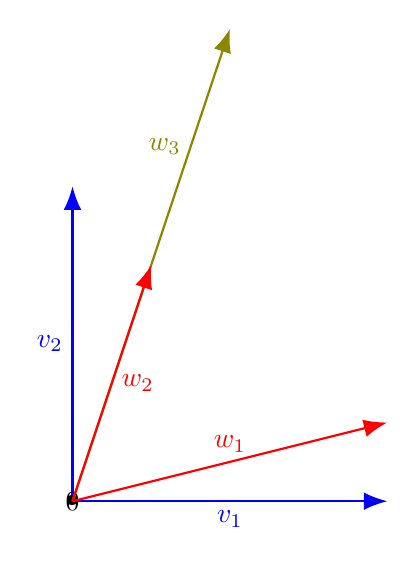
\begin{tikzpicture}
        \draw[-{Latex[length=3mm]}, thick,blue] (0,0) -- (4,0) ;
        \draw[-{Latex[length=3mm]}, thick,blue] (0,0) -- (0,4) ;
        \node at (0,0) {\textbullet};
        \node at (0,0) {$0$};
        \node[below,blue] at (2,0) {$v_1$};
        \node[left,blue] at (0,2) {$v_2$};
        \draw[-{Latex[length=3mm]}, thick, red] (0,0) -- (4,1) ;
        \node[above, red] at (2,0.5) {$w_1$};
        \node[right, red] at (0.5,1.5) {$w_2$};
        \draw[-{Latex[length=3mm]}, thick, olive] (0,0) -- (2,6) ;
        \draw[-{Latex[length=3mm]}, thick, red] (0,0) -- (1,3) ;
        \node[left, olive] at (1.5,4.5) {$w_3$};
      \end{tikzpicture}
    }
  \end{center}

  \begin{itemize}
  \item $\{ v_1,v_2\}$ is a basis
  \item $\{ w_1,w_2\}$ is a basis
  \item $\{ w_1,w_3\}$ is a basis
  \item $\{ w_2,w_3\}$ is NOT a basis
  \end{itemize}
\end{frame}

\begin{frame}
  {Every Finite Dimensional Vector Space Has a Basis}

  \begin{itemize}
  \item Assume that $T$ is a finite dimensional vector space
    \begin{itemize}
    \item By the definition of a finite-dimensional vector space,
      there is a finite set $S = \{ s_1, \dots, s_p\}$ that spans $T$
    \item If \eqref{independence} holds, then $S$ is a basis
    \item If \eqref{independence} does not hold, then there exists $f^1, \dots, f^p \in \F$, not all zero, such that
      \[ 
        f^1 s_1 + \cdots f^ps_p = \zero
      \]
    \item Suppose $f^p \ne 0$
    \item It follows that
      \[
        s_p = \frac{f^1}{f^p}s_1 + \cdots + \frac{f^{p-1}}{f^p}s_{p-1} = \zero
      \]
    \item It follows that $S' = \{ s_1, \dots, s_{p-1} \}$ spans $T$
    \item If $S'$ is not a basis, then repeat previous steps
    \item After a finite number of steps, you get either a basis or $S = \{\zero\}$
    \end{itemize}
  \end{itemize}
\end{frame}

\begin{frame}
  {Dimension of a Vector Space}

  \begin{itemize}
  \item Every basis of a finite dimensional vector space $V$ has the same number of elements
  \item If $(v_1, \dots, v_m)$ and $(w_1, \dots, w_n)$ are bases of $V$, then $m = n$
  \item We define the dimension of a finite dimensional vector space $V$ to be the number of elements in a basis
  \item The dimension of $V$ is denoted $\dim V$
  \end{itemize}
\end{frame}

\section{Matrix Notation}

\begin{frame}
  {Matrix Product of a Row Matrix and a Column Matrix}

  \begin{itemize}
  \item A row matrix looks like this:
    \[
      R = (r_1, \dots, r_m) = \begin{bmatrix} r_1 & \cdots & r_m\end{bmatrix}
    \]
  \item A column matrix looks like this:
    \[
      C = \langle c^1, \dots, c^m\rangle = \begin{bmatrix} c^1\\ \vdots \\ c^m\end{bmatrix}
    \]
  \item The matrix product of $R$ and $C$ looks like this
    \[
      RC = \begin{bmatrix} r_1 & \cdots & r_m\end{bmatrix}\begin{bmatrix} c^1\\ \vdots \\ c^m\end{bmatrix} = r_1c^1 + \cdots + r_mc^m
    \]
  \item Normally, $r_1, \dots, r_m, c^1, \dots, c^m$ are scalars, but the notation can also be used, as long as you can multiply each $r_k$ by each $c^k$
  \end{itemize}
\end{frame}


\begin{frame}
  {Generalized Matrix Products}

  \begin{itemize}
  \item This notation works if
    \begin{enumerate}\setlength{\itemsep}{5pt}
    \item
      \begin{itemize}
      \item Each $r_k$ is a scalar
      \item Each $c^k$ is a scalar
      \item And therefore $RC$ is a scalar
      \end{itemize}
    \item
      \begin{itemize}
      \item Each $r_j$ is a scalar
      \item Each $c^k$ is a vector
      \item And therefore $RC$ is a vector
      \end{itemize}
    \item
      \begin{itemize}
      \item Each $r_j$ is a vector
      \item Each $c^k$ is a scalar
      \item And therefore $RC$ is a vector
      \end{itemize}
    \end{enumerate}
  \item The notation is invalid if
    \begin{itemize}
    \item Each $r_j$ is a vector
    \item Each $c^k$ is a vector
    \end{itemize}
  \item Order matters: $CR \ne RC$!
  \item We will use only items 1 and 3 above
  \end{itemize}
\end{frame}

\begin{frame}
  {Abstract Notation}

  \begin{itemize}
  \item A basis $(e_1, \dots, e_m)$ of a vector space $V$ will always be written as a row matrix of vectors,
    \[ E = \bbm e_1 & \cdots & e_m \ebm \]
  \item Any vector $v = e_1a^1 + \cdots + e_ma^m\in V$ can be written as
    \begin{align*}
      v &= e_1a^1 + \cdots + e_ma^m
          = \bbm e_1 & \cdots & e_m \ebm\bbm a^1 \\ \vdots \\ a^m \ebm
      = Ea
    \end{align*}
  \end{itemize}
\end{frame}

\section{Change of Basis}

\begin{frame}
  {Example of Change of Basis}

  \begin{itemize}
  \item Let $E$ be the standard basis of $\F^3$ and
    \[
      F = \begin{bmatrix} f_1 & f_2 & f_3 \end{bmatrix}
      = \left[ \begin{array}{c|c|c} 1 & 0 & 0 \\ -1 & 1 & 0 \\ 1 & 1 & 1 \end{array}\right]
    \]
  \item Given a vector $v = (1,2,3)$, there are coefficients $b^1, b^2, b^3$ such that
    \begin{align*}
      (1,2,3) &= b^1(1,-1,1) + b^2(0,1,1) + b^3(0,0,1)\\
              &= (b^1, -b^1+b^2, b^1+b^3+b^3)
    \end{align*}
    or, equivalently,
    \begin{align*}
      b^1 &= 1\\
      -b^1 + b^2 &= 2\\
      b^1 + b^2 + b^3 &= 3
    \end{align*}
  \item Unique solution is $(b^1,b^2,b^3) = (1, 3, -1)$
  \end{itemize}
\end{frame}

\begin{frame}
  {Change of Basis}

  \begin{itemize}
  \item Consider two different bases of an $n$-dimensional vector space $V$,
    \[
      E = \begin{bmatrix} e_1 & \cdots & e_n \end{bmatrix}\text{ and }
      F  \begin{bmatrix} f_1 & \cdots & f_n \end{bmatrix}
    \]
  \item Since $F$ is a basis, we can write each vector in $F$ as a linear combination of the vectors in $E$
    \begin{align*}
      F &= \begin{bmatrix} f_1 & \cdots & f_n\end{bmatrix}\\
        &= \begin{bmatrix} e_1M_1^1 + \cdots + e_nM_1^n & \cdots & e_1M_n^1 + \cdots + e_nM_n^n \end{bmatrix}\\
        &= \begin{bmatrix} e_1 & \cdots & e_n \end{bmatrix}
          \begin{bmatrix} M^1_1 & \cdots & M^1_n \\ \vdots & & \vdots \\ M^n_1 & \cdots & M^n_n \end{bmatrix}\\
        &= EM
    \end{align*}
  \end{itemize}
\end{frame}

\begin{frame}
  {Change of Coefficients}

  \begin{itemize}
  \item Any vector $v$ can be written as a linear combination of the vectors in $E$ or as a linear combination of the vectors in $F$
    \begin{align*}
      v &= e_1a^1 + \cdots + e_na^n = \begin{bmatrix} e_1 & \cdots & e_n \end{bmatrix}\begin{bmatrix} a^1 \\ \vdots \\ a^n\end{bmatrix} = Ea\\
      \text{ or }
      v &= f_1b^1 + \cdots + f_nb^n = \begin{bmatrix} f_1 & \cdots & f_n \end{bmatrix}\begin{bmatrix} b^1 \\ \vdots \\ b^n\end{bmatrix} = Fb\\
    \end{align*}
  \item If $F = EM$, then
    \[
      v = Fb = E(Mb)\ \leadsto\ a = Mb\text{ and }b = M^{-1}a
    \]
  \end{itemize}
\end{frame}

\begin{frame}
  {Change of Basis Formula}

  \begin{itemize}
  \item If $E$ and $F$ are bases of $V$ such that
    \[
      F = EM,
    \]
    then given any vector $v = Ea$,
    \[
      v = Fb\text{, where }b = M^{-1}a
    \]
  \item The matrix that transforms old coefficients into new coefficients is the inverse of the matrix that transforms the old basis into the new basis
  \item This works only if you write a basis as a row matrix of vectors and the coefficients as a column matrix of scalars
  \end{itemize}
\end{frame}

\section{Linear Functions and Maps}

\begin{frame}
  {Linear Functions}

  \begin{itemize}
  \item If $V$ is a vector space, then a function
    \[ \ell: V \rightarrow \F \]
    is {\bf linear}, if for any $v, v_1, v_2 \in V$ and $s \in \F$,
    \begin{align*}
      \forall v_1, v_2 \in V,\ &\ell(v_1+v_2) = \ell(v_1) + \ell(v_2)\\
      \forall s \in \F, v \in V,\ &\ell(vs) = \ell(v)s
    \end{align*}
  \item Easy to check that $\ell(0_V) = 0$
  \end{itemize}
\end{frame}

\begin{frame}
  {Linear Maps}

  \begin{itemize}
  \item If $V$ and $W$ are vector spaces, then
    \[ L: V \rightarrow W \]
    is a {\bf linear map} or {\bf linear transformation}, if for any $v, v_1, v_2 \in V$ and $s \in \F$,
    \begin{align*}
      L(v_1+v_2) &= L(v_1) + L(v_2)\\
      L(sv) &= sL(v)
    \end{align*}
  \item Easy to check that $L(0_V) = 0_W$
  \item If $K: U \rightarrow V$ and $L: V \rightarrow W$ are linear maps, then so is
    \[ L\circ K: U \rightarrow W \]
  \item If $L: V \rightarrow W$ is bijective, it is called a {\bf linear isomorphism}
  \item If $L: V \rightarrow W$ is a linear isomorphism, then so is
    \[ L^{-1}: W \rightarrow V \]
  \end{itemize}
\end{frame}

\begin{frame}
  {$n$-Dimensional Vector Spaces are Isomorphic}

  \begin{itemize}
  \item Let $\dim V = \dim W = m$
  \item Let $E = (e_1, \dots, e_m)$ be a basis of $V$
  \item Let $F = (f_1, \dots, f_m)$ be a basis of $W$
  \item There is a linear isomorphism
    \begin{align*}
      L_{E,F}: V &\rightarrow W\\
      e_1a^1+\cdots+e_ma^m &\mapsto f_1a^1+\cdots + f_ma^m
    \end{align*}
  \item Given any basis $(e_1, \dots, e_m)$ of $V$, there is a linear isomorphism
    \begin{align*}
      L_V: \F^m &\rightarrow V\\
      (a^1, \dots, a^m) &\mapsto e_1a^1+ \cdots + e_ma^m
    \end{align*}
  \end{itemize}
\end{frame}

\begin{frame}
  {Vector Space of Linear Maps}

  \begin{itemize}
  \item Given vector spaces $V$ and $W$, let
    \[ \L(V,W) = \{ L: V \rightarrow W\ :\ L\text{ is linear} \} \]
  \item $\L(V,W)$ is itself a vector space, because
    \begin{itemize}
    \item If $A, B \in \L(V,W)$ and $s \in \F$, then
      \[
        A + B,\ sA \in \L(V,W)
      \]
    \end{itemize}
  \item Let $\gl(n,m,\F)$ denote the vector space of $n$-by-$m$ matrices with components in $\F$
    \begin{itemize}
    \item $\dim \gl(n,m,\F) = nm$
    \end{itemize}
  \end{itemize}
\end{frame}

\begin{frame}
  {Matrix as Linear Map}

  \begin{itemize}
  \item Let $E = (e_1, \dots, e_m)$ be a basis of $V$
  \item Let $F = (f_1, \dots, f_n)$ be a basis of $W$
  \item For each $M \in \gl(n,m,\F)$, let $L: V \rightarrow W$ be the linear map where
    \[
      \forall\ 1 \le k \le m,\ L(e_k) = f_1M_k^1 + \cdots + f_nM_k^n
    \]
    and therefore for any $v = e_1a^1+\cdots e_ma^m = Ea$,
    \begin{align*}
      L(v) &= L(e_1a^1+ \cdots + e_ma^m)\\
           &= L(e_1)a^1 + \cdots + L(e_m)a^m\\
           &= (f_1M_1^1+\cdots+f_nM_1^n)a^1 + \cdots +(f_1M_m^1+\cdots+f_nM_m^n)a^m\\
           &= f_1(M_1^1a^1+\cdots+M_m^1a^m) + \cdots f_n(M_1^na^1+\cdots+M_m^na^m)\\
           &= f_1(Ma)^1+ \cdots + f_n(Ma)^n
    \end{align*}
  \item This defines a map $I_{E,F}: \gl(n,m,\F) \rightarrow \L(V,W)$
  \end{itemize}
\end{frame}

\begin{frame}
  {Linear Map as Matrix}

  \begin{itemize}
  \item Let $E = (e_1, \dots, e_m)$ be a basis of $V$
  \item Let $F = (f_1, \dots, f_n)$ be a basis of $W$
  \item Let $L: V \rightarrow W$ be a linear map
  \item For each $e_k$, $1 \le k \le m$, there exists $(M_k^1, \dots, M_k^n) \in \F^n$ such that
    \[ L(e_k) = f_1M_k^1 + \cdots f_nM_k^n \]
  \item Therefore, for any
    $v = e_1a^1 + \cdots + e_ma^m \in V$,
    \begin{align*}
      L(v) &= L(e_1a^1+\cdots+e_ma^m)\\
           &= L(e_1)a^1 + \cdots + L(e_m)e^m\\
           &= (f_1M_1^1+\cdots f_nM^n_1)a^1
             + \cdots + (f_1M_m^1+\cdots+f_nM_m^n)a^m\\
           &= f_1(M_1^1a^1 + \cdots M_m^1a^m) + \cdots + f_n(M_1^na^1+ \cdots + M_m^na^m)\\
           &= f_1(Ma)^1 + \cdots + f_n(Ma)^n
    \end{align*}
  \item This defines a map $J_{E,F}: \L(V,W) \rightarrow \gl(n,m,\F)$\\
  \item $J_{E,F} = I_{E,F}^{-1}$ and $I_{E,F} = J_{E,F}^{-1}$
  \item Therefore, $\dim \L(V,W) = \dim \gl(n,m,\F) = nm$
  \end{itemize}
\end{frame}

\begin{frame}
  {Concrete to Abstract Notation}

  \begin{align*}
    L(v) &= L(e_1a^1 + \cdots + e_ma^m)
           = L\left(\begin{bmatrix} e_1 & \cdots & e_m \end{bmatrix}\bbm a^1 \\ \vdots \\ a^m\ebm\right)\\
         & = L\left(\begin{bmatrix} e_1 & \cdots & e_m \end{bmatrix}\right)\bbm a^1 \\ \vdots \\ a^m\ebm
    = \bbm L(e_1) & \cdots & L(e_m) \ebm\bbm a^1 \\ \vdots \\ a^m\ebm\\
         &= \bbm f_1M^1_1+ \cdots+f_nM^n_1 & \cdots & f_1M^1_n+\cdots+f_nM^n_n \ebm\bbm a^1 \\ \vdots \\ a^m\ebm\\
         &= \bbm f_1 & \cdots & f_n\ebm\bbm M^1_1 & \cdots & M^1_m \\ \vdots & & \vdots \\ M^n_1 & \cdots & M^n_m \ebm \bbm a^1 \\ \vdots \\ a^m\ebm
    = FMa
  \end{align*}
\end{frame}

\begin{frame}
  {Subspace and its Dimension}

  \begin{itemize}
  \item A subset $T$ of a vector space $X$ is a {\bf subspace} of $X$ if for any $p, q \in \F$ and $a, b \in T$,
    \[
      pa + qb \in T
    \]
  \item If a subspace has at least one nonzero vector, then it is itself a vector space
  \item Define the dimension of a subspace $S$ as follows:
    \begin{itemize}
    \item If $S = \{\zero\}$ then $\dim S = 0$
    \item If $S \ne \{\zero\}$, then $S$ is a vector space and $\dim S$ is its dimension as a vector space
    \end{itemize}
  \end{itemize}
\end{frame}

\begin{frame}
  {Kernel, Image, Rank of a Linear Map}

  \begin{itemize}
  \item Consider any linear map $P: Z \rightarrow Y$
  \item The {\bf kernel} of $P$ is defined to be
    \[
      \ker P = \{ z \in Z\ :\ P(z) = \zero \}
    \]
    \begin{itemize}
    \item $\ker(P)$ is a subspace of $Z$
    \end{itemize}
  \item The {\bf image} of $P$ is defined to be
    \begin{align*}
      P(Z) &= \{ P(z)\ :\ z \in Z\} \subset Y
    \end{align*}
    \begin{itemize}
    \item $P(Z)$ is a subspace of $Y$
    \end{itemize}
  \item The {\bf rank} of $P$ is
    \[
      \rank(P) = \dim P(Z)
    \]
  \end{itemize}
\end{frame}

\begin{frame}
  {Example 0}

  \begin{itemize}
  \item Define $Z: \F^2 \rightarrow \F^3$ to be
    \[
      Z(x,y) = (x,y,0)\text{, for all }(x,y) \in \F^2
    \]
  \item In other words,
    \[
      Z\left(\begin{bmatrix} x \\ y \end{bmatrix}\right)
      =
      \begin{bmatrix} 1 & 0 \\ 0 & 1 \\ 0 & 0 \end{bmatrix}\begin{bmatrix} x \\ y \end{bmatrix}
    \]
  \item $\ker Z = \{0\}$
  \item $Z(\F^2) = \{ (x,y,0)\ : x,y, \in \F\} \subset \F^n$
    \begin{itemize}
    \item A basis of $Z(\F^2)$ is $\{Z(e_1), Z(e_2)\} = \{(1,0,0), (0,1,0)\}$
    \end{itemize}
  \item Therefore,
    \begin{align*}
      \dim\ker Z &= 0\\
      \rank Z &= 2
    \end{align*}
  \end{itemize}
\end{frame}

\begin{frame}
  {Example 1}
  \begin{itemize}
  \item Define $W: \F^2 \rightarrow \F^3$ to be
    \[
      W(x,y) = (y,0,0)\text{, for all }(x,y) \in \F^2
    \]
  \item In other words,
    \[
      W\left(\begin{bmatrix} x \\ y \end{bmatrix}\right)
      =
      \begin{bmatrix} 0 & 1 \\ 0 & 0 \\ 0 & 0 \end{bmatrix}\begin{bmatrix} x \\ y \end{bmatrix}
    \]
  \item $\ker W = \{ (x,0)\ :\ x \in \F\}$
    \begin{itemize}
    \item A basis of $\ker W$ is $\{(1,0)\}$
    \end{itemize}
  \item $W(\F^2) = \{ (y,0,0)\ :\ y \in \F\}$
    \begin{itemize}
    \item A basis of $W(\F^2)$ is $\{(1,0,0)\}$
    \end{itemize}
  \item Therefore,
    \begin{align*}
      \dim \ker W &= 1\\
      \rank W &= 1
    \end{align*}
  \end{itemize}
\end{frame}

\begin{frame}
  {Example 2}
  \begin{itemize}
  \item Define $U: \F^2 \rightarrow \F^3$ to be
    \[
      U(x,y) = (0,0,0)\text{, for all }(x,y) \in \F^2
    \]
  \item In other words,
    \[
      U\left(\begin{bmatrix} x \\ y \end{bmatrix}\right)
      =
      \begin{bmatrix} 0 & 0 \\ 0 & 0 \\ 0 & 0 \end{bmatrix}\begin{bmatrix} x \\ y \end{bmatrix}
    \]
  \item $\ker U = \F^2$
  \item $U(\F^2) = \{ (0,0,0\}$
  \item Therefore,
    \begin{align*}
      \dim \ker U &= 2\\
      \rank U &= 0
    \end{align*}
  \end{itemize}
\end{frame}

\begin{frame}
  {Example 3}
  \begin{itemize}
  \item Define $U: \F^3 \rightarrow \F^2$ to be
    \[
      U(x,y,z) = (y,z)\text{, for all }(x,y,z) \in \F^3
    \]
  \item In other words,
    \[
      U\left(\begin{bmatrix} x \\ y \\ z\end{bmatrix}\right)
      =
      \begin{bmatrix} 0 &  1 & 0\\ 0 & 0 & 1 \end{bmatrix}\begin{bmatrix} x \\ y \\ z\end{bmatrix}
    \]
  \item $\ker U = \{ (x,0,0)\ :\ z\in \F\}$
    \begin{itemize}
    \item A basis is $\{ (1,0,0) \}$
    \end{itemize}
  \item $U(\F^3) = \F^2 $
  \item Therefore,
    \begin{align*}
      \dim \ker U &= 1\\
      \rank U &= 2
    \end{align*}
  \end{itemize}
\end{frame}

\begin{frame}
  {Example 4}
  \begin{itemize}
  \item Define $U: \F^3 \rightarrow \F^2$ to be
    \[
      U(x,y,z) = (z,0)\text{, for all }(x,y,z) \in \F^3
    \]
  \item In other words,
    \[
      U\left(\begin{bmatrix} x \\ y \\ z\end{bmatrix}\right)
      =
      \begin{bmatrix} 0 & 0 & 1\\ 0 & 0 & 0 \end{bmatrix}\begin{bmatrix} x \\ y \\ z\end{bmatrix}
    \]
  \item $\ker U = \{ (x,y,0)\ :\ x,y\in \F\}$
    \begin{itemize}
    \item A basis is $\{ (1,0,0), (0,1,0)\}$
    \end{itemize}
  \item $U(\F^2) = \{ (z,0)\ :\ z \in \F \}$
    \begin{itemize}
    \item A basis is $\{ (1,0)\}$
    \end{itemize}
  \item Therefore,
    \begin{align*}
      \dim \ker U &= 2\\
      \rank U &= 1
    \end{align*}
  \end{itemize}
\end{frame}

\begin{frame}
  {Example 5}
  \begin{itemize}
  \item Define $U: \F^3 \rightarrow \F^2$ to be
    \[
      T(x,y,z) = (0,0,0)\text{, for all }(x,y,z) \in \F^3
    \]
  \item In other words,
    \[
      T\left(\begin{bmatrix} x \\ y \\ z\end{bmatrix}\right)
      =
      \begin{bmatrix} 0 & 0 & 0\\ 0 & 0 & 0 \end{bmatrix}\begin{bmatrix} x \\ y \\ z\end{bmatrix}
    \]
  \item $\ker U = \F^3$
  \item $U(\F^3) = \{ (0,0,0) \}$
  \item Therefore,
    \begin{align*}
      \dim \ker U &= 3\\
      \rank U &= 0
    \end{align*}
  \end{itemize}
\end{frame}

\section{Linear Maps}

\begin{frame}
  {Bases of $V$ and $W$ Induce Basis of $\L(V,W)$}

  \begin{itemize}
  \item If $(e_1, \dots, e_m)$ is a basis of $V$ and $(f_1, \dots, f_n)$ is a basis of $W$, then for each $1 \le k \le m$ and $1 \le p \le n$, let
    \[
      L_k^p: V \rightarrow W
    \]
    be the linear map where
    \[
      L^k_p(e_j) =
      \begin{cases}
        f_p&\text{ if }j = k\\
        0 &\text{ otherwise}
      \end{cases}
    \]
    and let $E^p_k \in \gl(n,m)$ be the matrix that has a $1$ in the $p$-th row and $k$-th column and $0$ everywhere else
  \item The set
    $\{ L^k_p\ :\ 1 \le k \le m\text{ and }1 \le p \le n \}$
    is a basis of $\L(V,W)$ such that
    \[
      I_{V,W}(E^p_k) = M^p_k
    \]
  \end{itemize}
\end{frame}

\begin{frame}
  {Normal Form of a Linear Map}

  \begin{itemize}
  \item Let $L: V \rightarrow W$ be a linear map
  \item Lemma: There exists a basis $(e_1, \dots, e_m)$ of $V$ and a basis $(f_1, \dots, f_n)$ of $W$ such that for each $1 \le k \le m$,
    \begin{align*}
      L(e_k)
      &=
        \begin{cases}
          f_k &\text{ if }1 \le k \le r\\
          0_W &\text{ if }r+1 \le k \le m
        \end{cases},
    \end{align*}
    where $r = \rank(L)$
  \item In particular,
    \[ \ker(L) = \text{ span of }\{e_{r+1}, \dots, e_m \} \text{ and }L(V) = \text{ span of }\{f_1, \dots, f_r\} \]
  \item The matrix of $L$ with respect to this basis is
    \[
      M = \left[\begin{array}{c|c} I_{r\times r} & 0_{r\times m-r} \\ \hline 0_{n-r,r} & 0_{n-r,m-r} \end{array}\right]
    \]
  \end{itemize}
\end{frame}

\begin{frame}
  {Corollary: Rank-Nullity Theorem}

  \begin{itemize}
  \item Theorem: $\dim \ker(L) + \rank(L) = \dim V$
  \item Proof: The normal form shows that if $\dim V = m$ and $\rank(L) = r$, then $\dim \ker(L) = m-r$
  \end{itemize}
\end{frame}

\begin{frame}
  {Proof of Existence of Normal Form}

  \begin{itemize}
  \item Let $s = \dim ker(L)$ and $r = \dim V - \dim \ker(L) = m-s$
  \item If $s > 0$, there exists a basis of $\ker(L)$, which will be denoted
    \[ (e_{m-s+1}, \dots, e_m) \]
  \item This can be extended to a basis $(e_1, \dots, e_r, e_{r+1}, \dots, e_m)$ of $V$
  \item For each $1 \le k \le r$, let $f_k = L(e_k)$
  \item $(f_1, \dots, f_r)$ is linearly independent
  \item It can be extended to a basis $(f_1, \dots, f_n)$ of $W$
  \item It follows that
    \begin{align*}
      \dim \ker L + \rank L &= \dim \ker L + \dim L(V)\\
                            &= s + r = m \\
                            &= \dim V
    \end{align*}
  \end{itemize}
\end{frame}

\begin{frame}
  {Injective and Surjective Maps}

  \begin{itemize}
  \item Consider a linear map $L: V \rightarrow W$
  \item $\dim \ker L = 0 \iff L$ is injective:
    \begin{align*}
      L(v_1) = L(v_2)
      & \iff L(v_2)-L(v_1) = 0_W\\
      &\iff L(v_2-v_1) = 0_W\\
      & \iff v_2-v_2 \in \ker L = \{0_V\}\\
      &\iff v_2 = v_1
    \end{align*}
  \item $\rank L = \dim W \iff L$ is surjective:
    \begin{align*}
      \rank L &= \dim W\\
      \iff \dim L(V) &= \dim W\\
      \iff L(V) &= W
    \end{align*}
  \end{itemize}
\end{frame}

\begin{frame}
  {Bijective Maps}

  \begin{itemize}
  \item A map $L: V \rightarrow W$ an {\bf isomorphism} if it is {\bf bijective}, i.e., both injective and surjective
  \item Therefore,
    \begin{align*}
      L: V \rightarrow W\text{ is bijective} &\iff\ \dim\ker(L) = 0\text{ and }\rank(L) = \dim W
    \end{align*}
  \item By the rank-nullity theorem, this holds if and only if
    \[
      \rank(L) = \dim W
    \]
  \item Equivalently, $L$ is an isomorphism if and only if
    \[
      \dim V = \dim W\text{ and }\dim \ker L = 0
    \]
    if and only if
    \[
      \dim V = \dim W = \rank L
    \]
  \end{itemize}
\end{frame}

\begin{frame}
  {Example (Part 1)}

  \begin{itemize}
  \item Consider the map $L: \F^3 \rightarrow \F^2$ given by
    \[
      L\left(\begin{bmatrix} v^1 \\ v^2 \\ v^3 \end{bmatrix}\right)
      =
      \begin{bmatrix} 1 & 2 & 3 \\ 0 & 0 & 4 \end{bmatrix}
      \begin{bmatrix} v^1 \\ v^2 \\ v^3 \end{bmatrix}
      = \begin{bmatrix} v^1 + 2v^2 + 3v^3 \\ 4v^3 \end{bmatrix}
    \]
  \item $\ker L = \{ (v^1,v^2,v^3)\ :\ v^1 + 2v^2 = 0 \}$
  \item A basis of $\ker L$ is $\{ (-2,1,0) \}$
  \item A basis of $\F^3$ is $\{ (0,1,0), (0,0,1), (-2,1,0) \}$
  \item A basis of $L(\F^3)$ is
    \[
      \{ L(0,1,0), L(0,0,1) \} = \{ (2,0), (3, 4) \}
    \]
  \end{itemize}
\end{frame}

\begin{frame}
  {Example (Part 2)}

  \begin{itemize}
  \item If
    \begin{align*}
      \begin{bmatrix} e_1 & e_2 & e_3 \end{bmatrix}
      &= \left[\begin{array}{c|c|c} 0 & 0 & -2 \\ 1 & 0 & 1 \\ 0 & 1 & 0 \end{array}\right]
        \text{ and }
        \begin{bmatrix} f_1 & f_2 \end{bmatrix}
        = \left[\begin{array}{c|c} 2 & 3 \\ 0 & 4 \end{array}\right]
    \end{align*}
  \item Then
    \[
      \begin{bmatrix} L(e_1) & L(e_2) & L(e_3) \end{bmatrix}
      = \begin{bmatrix} f_1 & f_2 & 0 \end{bmatrix} = \begin{bmatrix} f_1 & f_2 \end{bmatrix}
      \begin{bmatrix} 1 & 0 & 0 \\ 0 & 1 & 0 \end{bmatrix}
    \]
  \item And given any vector $v = e_1a^1 + e_2a^2 + e_3a^3$,
    \begin{align*}
      L(v) &= L(e_1)a^1 + L(e_2)a^2 + L(e_3)a^3 = f_1a^2 + f_2a^3 = FMa,
    \end{align*}
    where
    \[
      M = \begin{bmatrix} 0 & 1 & 0 \\ 0 & 0 & 1 \end{bmatrix}
    \]
  \end{itemize}
\end{frame}

\begin{frame}
  {Composition is Matrix Multiplication}

  \begin{itemize}
  \item Consider vector spaces $U, V, W$ and linear maps
    \[
      K: U \rightarrow V,\ L: V \rightarrow W
    \]
  \item Let $(e_1, \dots, e_k)$ be a basis of $U$
  \item Let $(f_1, \dots, f_m)$ be a basis of $V$
  \item Let $(g_1, \dots, g_n)$ be a basis of $W$
  \item There is an $m$-by-$k$ matrix $M$ such that
    \[
      K(e_j) = f_pM^p_j,\ 1 \le j \le k
    \]
  \item There is an $n$-by-$m$ matrix $N$ such that
    \[
      L(f_p) = g_aN^a_p,\ 1 \le p \le m
    \]
  \item There is an $n$-by-$k$ matrix $P$ such that
    \[
      (L\circ K)(e_j) = g_aP^a_j,\ 1 \le j \le k
    \]
  \item On the other hand,
    \begin{align*}
      (L\circ K)(e_j) &= L(K(e_j)) = L(f_pM^p_j) = L(f_p)M^p_j = g_aN^a_pM^p_j
    \end{align*}
  \item Therefore, $P^a_j = N^a_pM^p_j$.
  \end{itemize}
\end{frame}

\section{Determinants}

\begin{frame}
  \frametitle{Parallelogram in Vector Space}

  \begin{center}%
    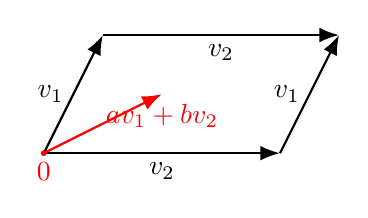
\begin{tikzpicture}[scale=0.75]
      \draw[-{Latex[length=2.5mm]}, thick] (-2,-1) -- (-1,1) ;
      \draw[-{Latex[length=2.5mm]}, thick] (-1,1) -- (3,1) ;
      \draw[-{Latex[length=2.5mm]}, thick] (2,-1) -- (3,1) ;
      \draw[-{Latex[length=2.5mm]}, thick] (-2,-1) -- (2,-1) ;
      % \draw[-{Latex[length=2.5mm]}, dashed, red] (-1,-1) -- (3,-1) ;
      % \draw[-{Latex[length=2.5mm]}, dashed, red] (-1,-1) -- (-1,1) ;
      % \draw[-{Latex[length=2.5mm]}, dashed, red] (3,-1) -- (3,1) ;
      \draw[red,-{Latex[length=2.5mm]}, thick] (-2,-1) -- (0,0) ;
      \node[below,red] at (0,0) {$av_1+bv_2$};
      \fill[red] (-2,-1) circle(.05);
      \node[below,red] at (-2,-1) {$0$};
      \node[below] at (0,-1) {$v_2$};
      \node[below] at (1,1) {$v_2$};
      \node[left] at (-1.5,0) {$v_1$};
      \node[left] at (2.5,0) {$v_1$};
    \end{tikzpicture}
  \end{center}

  \begin{itemize}
  \item Let $V$ be a $2$-dimensional vector space
  \item Let $P(v_1,v_2)$ be the parallelogram with sides $v_1, v_2 \in V$.
    \[
      P(v_1,v_2) = \{ av_1 + bv_2\ :\ 0 \le a, b \le 1 \}.
    \]
  \end{itemize}

\end{frame}

\begin{frame}
  \frametitle{Parallelogram With Respect To Basis}

  \begin{center}%
    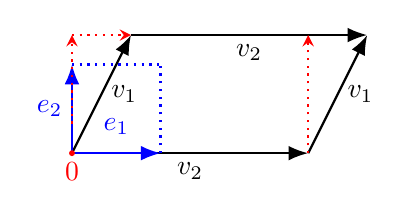
\begin{tikzpicture}[scale=0.75]
      \draw[-{Latex[length=2.5mm]}, thick] (-2,-1) -- (-1,1) ;
      \draw[-{Latex[length=2.5mm]}, thick] (-1,1) -- (3,1) ;
      \draw[-{Latex[length=2.5mm]}, thick] (2,-1) -- (3,1) ;
      \draw[-{Latex[length=2.5mm]}, thick] (-2,-1) -- (2,-1) ;
      % \draw[-{Latex[length=2.5mm]}, dashed, red] (-1,-1) -- (3,-1) ;
      % \draw[-{Latex[length=2.5mm]}, dashed, red] (-1,-1) -- (-1,1) ;
      % \draw[-{Latex[length=2.5mm]}, dashed, red] (3,-1) -- (3,1) ;
      \draw[blue,-{Latex[length=2.5mm]}, thick] (-2,-1) -- (-2,0.5) ;
      \node[left,blue] at (-2,-0.25) {$e_2$};
      \draw[blue,-{Latex[length=2.5mm]}, thick] (-2,-1) -- (-0.5,-1) ;
      \node[below,blue] at (-1.25,-0.25) {$e_1$};
      \draw[blue,dotted, thick] (-0.5,-1) -- (-0.5,0.5) ;
      \draw[blue,dotted, thick] (-2,0.5) -- (-0.5,0.5) ;
      \draw[red,dotted, thick,->] (-2,-0.5) -- (-2,1) ;
      \draw[red,dotted, thick,->] (-2,1) -- (-1,1) ;
      \draw[red,dotted, thick,->] (2,-1) -- (2,1) ;
      % \draw[dotted,red, thick,->] (2,-1) -- (3,-1) ;
      \fill[red] (-2,-1) circle(.05);
      \node[below,red] at (-2,-1) {$0$};
      \node[below] at (0,-1) {$v_2$};
      \node[below] at (1,1) {$v_2$};
      \node[right] at (-1.5,0) {$v_1$};
      \node[right] at (2.5,0) {$v_1$};
    \end{tikzpicture}
  \end{center}

  \begin{itemize}
  \item With respect to basis $(e_1,e_2)$
    $$v_1 = ae_1 + he_2\text{ and }v_2 = we_1$$
  \item Height is $h$ and width is $w$
  \item Assume area of $P(e_1,e_2)$ is
    \[
      A(e_1,e_2) = \area(P(e_1,e_2)) = 1
    \]
    
  \item Then the area of $P(v_1,v_2)$ is
    \[
      A(v_1,v_2) = \area(P(v_1,v_2)) = hw
    \]
  \end{itemize}
\end{frame}

\begin{frame}
  \frametitle{Upside Down Parallelogram With Respect To Basis}

  \begin{center}%
    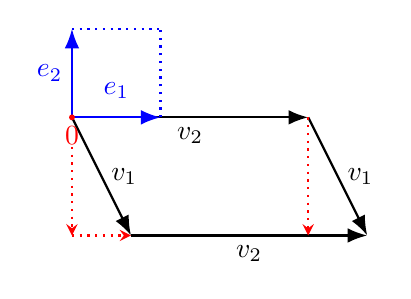
\begin{tikzpicture}[scale=0.75]
      \draw[-{Latex[length=2.5mm]}, thick] (-2,-1) -- (-1,-3) ;
      \draw[-{Latex[length=2.5mm]}, thick] (-1,-3) -- (3,-3) ;
      \draw[-{Latex[length=2.5mm]}, thick] (2,-1) -- (3,-3) ;
      \draw[-{Latex[length=2.5mm]}, thick] (-2,-1) -- (2,-1) ;
      \draw[blue,-{Latex[length=2.5mm]}, thick] (-2,-1) -- (-2,0.5) ;
      \node[left,blue] at (-2,-0.25) {$e_2$};
      \draw[blue,-{Latex[length=2.5mm]}, thick] (-2,-1) -- (-0.5,-1) ;
      \node[below,blue] at (-1.25,-0.25) {$e_1$};
      \draw[blue,dotted, thick] (-0.5,-1) -- (-0.5,0.5) ;
      \draw[blue,dotted, thick] (-2,0.5) -- (-0.5,0.5) ;
      \draw[red,dotted, thick,->] (-2,-1.5) -- (-2,-3) ;
      \draw[red,dotted, thick,->] (-2,-3) -- (-1,-3) ;
      \draw[red,dotted, thick,->] (2,-1) -- (2,-3) ;
      \fill[red] (-2,-1) circle(.05);
      \node[below,red] at (-2,-1) {$0$};
      \node[below] at (0,-1) {$v_2$};
      \node[below] at (1,-3) {$v_2$};
      \node[right] at (-1.5,-2) {$v_1$};
      \node[right] at (2.5,-2) {$v_1$};
    \end{tikzpicture}
  \end{center}

  \begin{itemize}
  \item With respect to basis $(e_1,e_2)$
    $$v_1 = ae_1 + he_2\text{ and }v_2 = we_1,$$
    where $h$ is negative
  \item Height is $|h|$ and width is $w$
  \item Then the area of $P(v_1,v_2)$ is
    \[
      A(v_1,v_2) = |h|w,
    \]
    whether $h$ is positive or negative
  \item Formula is awkward due to absolute value
  \end{itemize}
\end{frame}

\begin{frame}
  \frametitle{Oriented Area of Parallelogram}

  \begin{center}%
    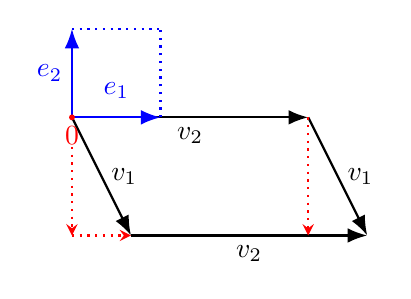
\begin{tikzpicture}[scale=0.75]
      \draw[-{Latex[length=2.5mm]}, thick] (-2,-1) -- (-1,-3) ;
      \draw[-{Latex[length=2.5mm]}, thick] (-1,-3) -- (3,-3) ;
      \draw[-{Latex[length=2.5mm]}, thick] (2,-1) -- (3,-3) ;
      \draw[-{Latex[length=2.5mm]}, thick] (-2,-1) -- (2,-1) ;
      \draw[blue,-{Latex[length=2.5mm]}, thick] (-2,-1) -- (-2,0.5) ;
      \node[left,blue] at (-2,-0.25) {$e_2$};
      \draw[blue,-{Latex[length=2.5mm]}, thick] (-2,-1) -- (-0.5,-1) ;
      \node[below,blue] at (-1.25,-0.25) {$e_1$};
      \draw[blue,dotted, thick] (-0.5,-1) -- (-0.5,0.5) ;
      \draw[blue,dotted, thick] (-2,0.5) -- (-0.5,0.5) ;
      \draw[red,dotted, thick,->] (-2,-1.5) -- (-2,-3) ;
      \draw[red,dotted, thick,->] (-2,-3) -- (-1,-3) ;
      \draw[red,dotted, thick,->] (2,-1) -- (2,-3) ;
      \fill[red] (-2,-1) circle(.05);
      \node[below,red] at (-2,-1) {$0$};
      \node[below] at (0,-1) {$v_2$};
      \node[below] at (1,-3) {$v_2$};
      \node[right] at (-1.5,-2) {$v_1$};
      \node[right] at (2.5,-2) {$v_1$};
    \end{tikzpicture}
  \end{center}

  \begin{itemize}
  \item Define oriented area to be
    \[
      A(v_1,v_2) = hw
    \]
  \item The oriented area of $P(v_1,v_2)$ is positive if $v_2$ lies counterclockwise of $v_1$
  \item The oriented area of $P(v_1,v_2)$ is negative if $v_2$ lies counterclockwise of $v_1$
  \item Oriented area, as a function of $v_1, v_2 \in V$ has nice properties
  \end{itemize}
\end{frame}

\begin{frame}
  \frametitle{Area of Two Parallelograms with Parallel Bases}

  \begin{center}
    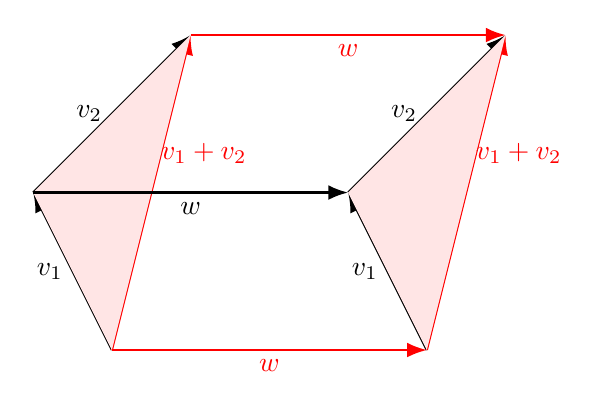
\begin{tikzpicture}
      \draw[-{Latex[length=2.5mm]}, thick] (-2,-1) -- (-3,1) ;
      \draw[-{Latex[length=2.5mm]}, thick] (-3,1) -- (-1,3) ;
      \draw[-{Latex[length=2.5mm]}, thick, red] (-2,-1) -- (-1,3) ;
      \fill[red!10] (-2,-1) -- (-3,1) -- (-1,3) -- cycle;
      \draw[-{Latex[length=2.5mm]}, thick] (-3,1) -- (1,1) ;
      \draw[-{Latex[length=2.5mm]}, thick] (2,-1) -- (1,1) ;
      \draw[-{Latex[length=2.5mm]}, thick] (1,1) -- (3,3) ;
      \draw[-{Latex[length=2.5mm]}, thick, red] (2,-1) -- (3,3) ;
      \fill[red!10] (2,-1) -- (1,1) -- (3,3) -- cycle;
      \draw[red,-{Latex[length=2.5mm]}, thick] (-2,-1) -- (2,-1) ;
      \draw[red,-{Latex[length=2.5mm]}, thick] (-1,3) -- (3,3) ;
      \node[red,below] at (0,-1) {$w$};
      \node[red,below] at (1,3) {$w$};
      \node[below] at (-1,1) {$w$};
      \node[left] at (-2.5,0) {$v_1$};
      \node[left] at (1.5,0) {$v_1$};
      \node[left] at (-2,2) {$v_2$};
      \node[left] at (2,2) {$v_2$};
      \node[red,right] at (-1.5,1.5) {$v_1+v_2$};
      \node[red,right] at (2.5,1.5) {$v_1+v_2$};
    \end{tikzpicture}
  \end{center}

  \begin{itemize}
  \item If $v_1$ and $v_2$ both point upward relative to $w$, then
    \[
      A(v_1+v_2,w) = A(v_1,w) + A(v_2,w)
    \]
  \end{itemize}
\end{frame}

\begin{frame}
  \frametitle{Area of Two Parallelograms with Parallel Bases}

  \begin{center}
    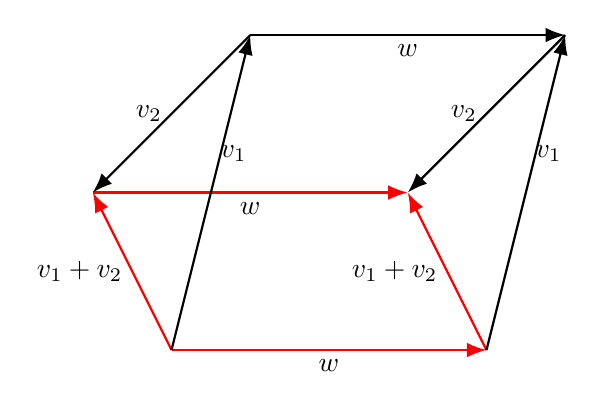
\begin{tikzpicture}
      \draw[red,-{Latex[length=2.5mm]}, thick] (-2,-1) -- (-3,1) ;
      \draw[red,-{Latex[length=2.5mm]}, thick] (-3,1) -- (1,1) ;
      \draw[red,-{Latex[length=2.5mm]}, thick] (2,-1) -- (1,1) ;
      \draw[red,-{Latex[length=2.5mm]}, thick] (-2,-1) -- (2,-1) ;
      \draw[{Latex[length=2.5mm]}-, thick] (-3,1) -- (-1,3) ;
      \draw[{Latex[length=2.5mm]}-, thick] (1,1) -- (3,3) ;
      \draw[-{Latex[length=2.5mm]}, thick] (-1,3) -- (3,3) ;
      \draw[-{Latex[length=2.5mm]}, thick] (-2,-1) -- (-1,3) ;
      \draw[-{Latex[length=2.5mm]}, thick] (2,-1) -- (3,3) ;
      \node[below] at (0,-1) {$w$};
      \node[below] at (1,3) {$w$};
      \node[below] at (-1,1) {$w$};
      \node[left] at (-2.5,0) {$v_1+v_2$};
      \node[left] at (1.5,0) {$v_1+v_2$};
      \node[left] at (-2,2) {$v_2$};
      \node[left] at (2,2) {$v_2$};
      \node[right] at (-1.5,1.5) {$v_1$};
      \node[right] at (2.5,1.5) {$v_1$};
    \end{tikzpicture}
  \end{center}

  \begin{itemize}
  \item If $v_1$ points upward and $v_2$ points downward relative to $w$, then $A(v_2,w) < 0$ and
    \[
      A(v_1,w) = A(v_1+v_2,w) - A(v_2,w)
    \]
    and therefore
    \[
      A(v_1+v_2,w) = A(v_1,w) + A(v_2,w)
    \]
  \end{itemize}
\end{frame}

\begin{frame}
  \frametitle{Area of rescaled parallelogram}

  \begin{center}
    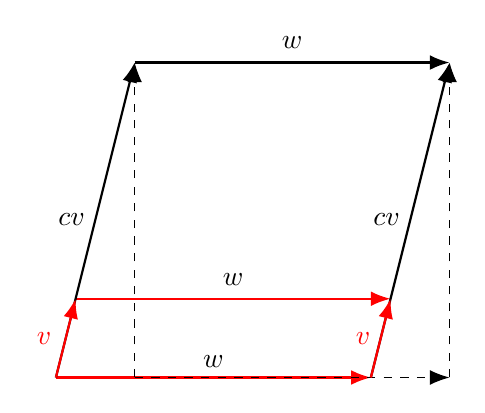
\begin{tikzpicture}
      \draw[-{Latex[length=2.5mm]}, thick, red] (-2,-1) -- (2,-1) ;
      \draw[-{Latex[length=2.5mm]}, thick, red] (-1.75,0) -- (2.25,0) ;
      \draw[-{Latex[length=2.5mm]}, thick] (-1,3) -- (3,3) ;
      \draw[-{Latex[length=2.5mm]}, dashed] (-1,-1) -- (-1,3) ;
      \draw[-{Latex[length=2.5mm]}, dashed] (3,-1) -- (3,3) ;
      \draw[-{Latex[length=2.5mm]}, dashed] (-1,-1) -- (3,-1) ;
      \draw[-{Latex[length=2.5mm]}, thick] (-2,-1) -- (-1,3) ;
      \draw[-{Latex[length=2.5mm]}, thick, red] (-2,-1) -- (-1.75,0) ;
      \draw[-{Latex[length=2.5mm]}, thick] (2,-1) -- (3,3) ;
      \draw[-{Latex[length=2.5mm]}, thick, red] (2,-1) -- (2.25,0) ;
      \node at (0,-0.8) {$w$};
      \node at (1,3.25) {$w$};
      \node at (0.25,0.25) {$w$};
      \node[red] at (-2.15,-0.5) {$v$};
      \node[red] at (1.9,-0.5) {$v$};
      \node at (-1.8,1) {$cv$};
      \node at (2.2,1) {$cv$};
    \end{tikzpicture}
  \end{center}

  \[
    A(cv,w) = cA(v,w)
  \]

\end{frame}

\begin{frame}
  \frametitle{Area of reflected parallelogram}

  \begin{center}
    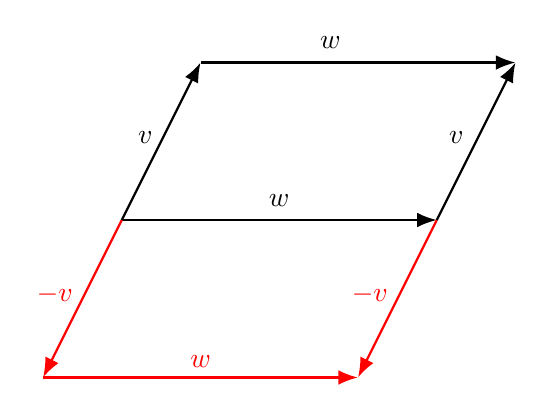
\begin{tikzpicture}
      \draw[-{Latex[length=2.5mm]}, thick, red] (-2,-1) -- (2,-1) ;
      \draw[-{Latex[length=2.5mm]}, thick] (-1,1) -- (3,1) ;
      \draw[-{Latex[length=2.5mm]}, thick] (0,3) -- (4,3) ;
      \draw[-{Latex[length=2.5mm]}, thick, red] (-1,1) -- (-2,-1) ;
      \draw[-{Latex[length=2.5mm]}, thick] (-1,1) -- (0,3) ;
      \draw[-{Latex[length=2.5mm]}, thick, red] (3,1) -- (2,-1) ;
      \draw[-{Latex[length=2.5mm]}, thick] (3,1) -- (4,3) ;
      \node[red] at (0,-0.8) {$w$};
      \node at (1.65,3.25) {$w$};
      \node at (1.0,1.25) {$w$};
      \node at (-0.7,2.05) {$v$};
      \node at (3.25,2.05) {$v$};
      \node[red] at (-1.85,0.05) {$-v$};
      \node[red] at (2.15,0.05) {$-v$};
    \end{tikzpicture}
  \end{center}

  \[
    A(-v,w) = A(v,w)
  \]

\end{frame}

\begin{frame}
  \frametitle{Area Versus Oriented Area}

  \begin{itemize}
  \item Definitions of area and oriented area require a basis $(e_1,e_2)$, where we assume that
    \[
      A(e_1,e_2) = 1
    \]
    \begin{itemize}
    \item In particular, $e_2$ must lie counterclockwise of $e_1$
    \end{itemize}
  \item The area function $|A(v,w)|$ is awkward to use
  \item Instead, define $A(v,w)$ to be the {\em oriented area} of $P(v,w)$
  \item Define the oriented area of $P(v,w)$ to be
    \[
      A(v,w) =
      \begin{cases}
        \text{area of }P(v,w) &\text{ if }(v,w)\text{ is positively oriented}\\
        -\text{area of }P(v,w) &\text{ if }(v,w)\text{ is negatively oriented}\\
        0 &\text{ if }v\text{ and }w\text{ are linearly dependent}
      \end{cases}
    \]
  \end{itemize}
\end{frame}

\begin{frame}
  \frametitle{Oriented Area of Parallelogram}

  \begin{itemize}
  \item If $w$ is held fixed, $A(v,w)$ is a linear function of $v$
    \begin{align*}
      A(v_1+v_2,w) &= A(v_1,w) + A(v_2,w)\\
      A(cv,w) &= cA(v,w)
    \end{align*}
  \item If $v$ is held fixed, $A(v,w)$ is a linear function of $w$
    \begin{align*}
      A(v,w_1+w_2) &= A(v,w_1) + A(v,w_2)\\
      A(v,cw) &= cA(v,w)
    \end{align*}
  \item Such a function of two vectors is called {\bf bilinear}    
  \item For any $v \in V$, the parallelogram $A(v,v)$ has height $0$ and therefore
    \begin{equation}\label{zero}
      A(v,v) = 0
    \end{equation}
  \item Fact: Any bilinear function $A: V\times V \rightarrow \F$ that satisfies \eqref{zero} is {\bf antisymmmetric}
  \item This means that for any $v, w \in V$,
    \[
      A(w,v) = -A(v,w)
    \]
  \end{itemize}
\end{frame}

\begin{frame}
  {$2$-Dimensional Antisymmetric Bilinear Function}

  \begin{itemize}
  \item Let $\begin{bmatrix} e_1 e_2 \end{bmatrix}$ be a basis of $V$
  \item Let
    \[ A: V\times V \rightarrow \F \]
    be an antisymmetric bilinear function such that
    \[ A(e_1,e_2)=1 \]
  \item If $v = ae_1+be_2$ and $w = ce_1+de_2$, then
    \begin{align*}
      A(v,w) &= A(ae_1 + be_2, ce_1 + de_2)\\
             &= A(ae_1,ce_1) + A(be_2,ce_1) + A(ae_1,de_2) + A(be_2,de_2)\\
             &= bcA(e_2,e_1) + adA(e_,e_2)\\
             &= ad-bc
    \end{align*}
  \end{itemize}
\end{frame}

\begin{frame}
  {$2$-Dimensional Antisymmetric Bilinear Function}

  \begin{itemize}
  \item This can be written as follows
    \begin{align*}
      A\left((\begin{bmatrix} v & w\end{bmatrix}\right)
      &= A\left(\begin{bmatrix} e_1 & e_2 \end{bmatrix}\begin{bmatrix} a & b \\ c & d \end{bmatrix}\right)\\
                                &= A\left(\begin{bmatrix} ae_1 + be_2  & ce_1 + de_2\end{bmatrix}\right)\\
                                &= A(e_1,e_2)(ad-bc)\\
                                &= ad-bc
    \end{align*}
  \item The determinant of a square $2$-by-$2$ matrix is defined to be
    \[
      \det \begin{bmatrix} a & b \\ c & d \end{bmatrix} = ad-bc
    \]
  \end{itemize}
\end{frame}

\begin{frame}
  {Determinant of a $2$-by-$2$ Matrix is Equal to Oriented Area}

  \begin{itemize}
  \item Let $(e_1,e_2)$ be a basis where the oriented area of $P(e_1,e_2)$ is $1$,
    \[ A(e_1,e_2) = 1 \]
  \item The oriented area of the parallelogram $P(v,w)$, where
    \[
      \begin{bmatrix} v & w \end{bmatrix} = \begin{bmatrix} e_1 & e_2 \end{bmatrix}
      \begin{bmatrix} a & b \\ c & d \end{bmatrix},
    \]
    is
    \[
      A(v,w) = \det \begin{bmatrix} a & b \\ c & d \end{bmatrix}
    \]
  \end{itemize}
\end{frame}

\begin{frame}
  \frametitle{Parallelopiped spanned by $3$ Vectors in $3$-space}

  \begin{center}
    \scalebox{0.75}
    {
      \tdplotsetmaincoords{0}{0}
      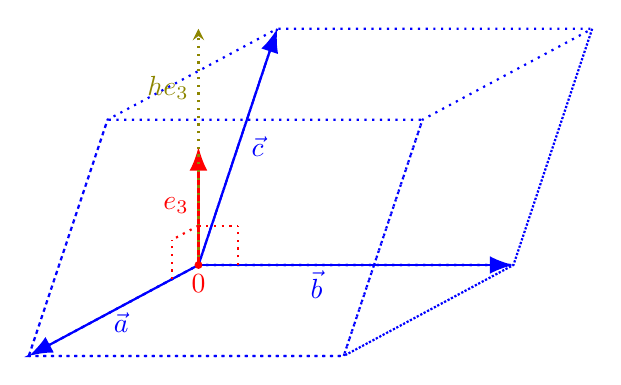
\begin{tikzpicture}%[rotate around y=-15, rotate around z=7]
        % [tdplot_main_coords]
        % Vectors
        % \node[red] at (0, 0, 3.5) {$x$};
        % \node[red] at (3.5, 0, 0) {$y$};
        % \node[red] at (0, 3.5, 0) {$z$};

        % \draw [-{Latex[length=3mm]}, red, thick] (0,0,0) -- (3,0,0);
        % \draw [-{Latex[length=3mm]}, red, thick] (0,0,0) -- (0,3,0);
        % \draw [-{Latex[length=3mm]}, red, thick] (0,0,0) -- (0,0,3);

        \draw [dotted, blue, thick] (0,0,0) -- (4,0,0) -- (3,0,3) -- (-1,0,3) -- cycle;
        \draw [dotted, blue, thick] (0,0,0) -- (4,0,0) -- (5,3,0) -- (1,3,0) -- cycle;
        \draw [dotted, blue, thick] (-1,0,3) -- (3,0,3) -- (4,3,3) -- (0,3,3) -- cycle;
        \draw [dotted, blue, thick] (1,3,0) --(0,0,0) -- (-1,0,3) -- (0,3,3) -- cycle;
        \draw [dotted,blue, thick] (5,3,0) --(4,0,0) -- (3,0,3) -- (4,3,3) -- cycle;
        \draw [-{Latex[length=3mm]}, blue, thick] (0,0,0) -- (-1,0,3);
        \node[blue] at (-0.5,-0.25,1.25) {$\vec{a}$};
        \draw [-{Latex[length=3mm]}, blue, thick] (0,0,0) -- (4,0,0);
        \node[blue] at (1.5,-0.25,0) {$\vec{b}$};
        \draw [-{Latex[length=3mm]}, blue, thick] (0,0,0) -- (1,3,0);
        \node[blue] at (0.75,1.5,0) {$\vec{c}$};
        \draw [-{Latex[length=3mm]}, red, thick] (0,0,0) -- (0,1.5,0);
        \node[red,left] at (0,0.75,0) {$e_3$};
        \draw [->,olive,dotted, thick] (0,0,0) -- (0,3,0);
        \node [left,olive] at (0,2.25,0) {$he_3$};

        \draw [red, thick, dotted] (0,0.5,0) -- ({-0.5/sqrt(10)},0.5,{1.5/sqrt(10)});
        \draw [red, thick, dotted] ({-0.5/sqrt(10)},0,{1.5/sqrt(10)}) -- ({-0.5/sqrt(10)},0.5,{1.5/sqrt(10)});
        \draw [red, thick, dotted] (0,0.5,0) -- (0.5,0.5,0);
        \draw [red, thick, dotted] (0.5,0,0) -- (0.5,0.5,0);
        \fill[red] (0,0,0) circle(.05);
        \node[below,red] at (0,0,0) {$0$};
      \end{tikzpicture}
    }
  \end{center}

  \begin{itemize}
  \item Three linearly independent vectors $\vec{a}, \vec{b}, \vec{c}$  span a parallelopiped $P(\vec{a},\vec{b},\vec{c})$
    \[
      P(\vec{a},\vec{b},\vec{c}) = \{ s\vec{a}+t\vec{b} +u\vec{c}\ :\ 0 \le s, t, u \le 1 \}
    \]
  \end{itemize}
\end{frame}

\begin{frame}
  \frametitle{Volume of a Parallelopiped}
  
  \begin{center}
    \scalebox{0.75}
    {
      \tdplotsetmaincoords{0}{0}
      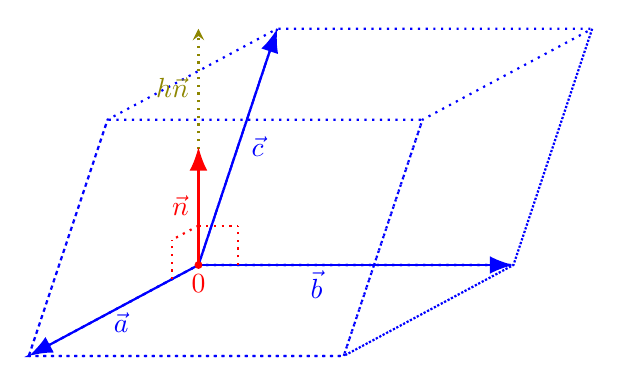
\begin{tikzpicture}%[rotate around y=-15, rotate around z=7]
        % [tdplot_main_coords]
        % Vectors
        % \node[red] at (0, 0, 3.5) {$x$};
        % \node[red] at (3.5, 0, 0) {$y$};
        % \node[red] at (0, 3.5, 0) {$z$};

        % \draw [-{Latex[length=3mm]}, red, thick] (0,0,0) -- (3,0,0);
        % \draw [-{Latex[length=3mm]}, red, thick] (0,0,0) -- (0,3,0);
        % \draw [-{Latex[length=3mm]}, red, thick] (0,0,0) -- (0,0,3);

        \draw [dotted, blue, thick] (0,0,0) -- (4,0,0) -- (3,0,3) -- (-1,0,3) -- cycle;
        \draw [dotted, blue, thick] (0,0,0) -- (4,0,0) -- (5,3,0) -- (1,3,0) -- cycle;
        \draw [dotted, blue, thick] (-1,0,3) -- (3,0,3) -- (4,3,3) -- (0,3,3) -- cycle;
        \draw [dotted, blue, thick] (1,3,0) --(0,0,0) -- (-1,0,3) -- (0,3,3) -- cycle;
        \draw [dotted,blue, thick] (5,3,0) --(4,0,0) -- (3,0,3) -- (4,3,3) -- cycle;
        \draw [-{Latex[length=3mm]}, blue, thick] (0,0,0) -- (-1,0,3);
        \node[blue] at (-0.5,-0.25,1.25) {$\vec{a}$};
        \draw [-{Latex[length=3mm]}, blue, thick] (0,0,0) -- (4,0,0);
        \node[blue] at (1.5,-0.25,0) {$\vec{b}$};
        \draw [-{Latex[length=3mm]}, blue, thick] (0,0,0) -- (1,3,0);
        \node[blue] at (0.75,1.5,0) {$\vec{c}$};
        \draw [->,olive,dotted, thick] (0,0,0) -- (0,3,0);
        \node [left,olive] at (0,2.25,0) {$h\vec{n}$};

        \draw [red, thick, dotted] (0,0.5,0) -- ({-0.5/sqrt(10)},0.5,{1.5/sqrt(10)});
        \draw [red, thick, dotted] ({-0.5/sqrt(10)},0,{1.5/sqrt(10)}) -- ({-0.5/sqrt(10)},0.5,{1.5/sqrt(10)});
        \draw [red, thick, dotted] (0,0.5,0) -- (0.5,0.5,0);
        \draw [red, thick, dotted] (0.5,0,0) -- (0.5,0.5,0);
        \fill[red] (0,0,0) circle(.05);
        \node[below,red] at (0,0,0) {$0$};
        \draw [-{Latex[length=3mm]}, red, thick] (0,0,0) -- (0,1.5,0);
        \node[red,left] at (0,0.75,0) {$\vec{n}$};
      \end{tikzpicture}
    }
  \end{center}

  \begin{itemize}
  \item Fix a basis $(e_1,e_2,e_3)$ of $V$
    \begin{itemize}
    \item Assume the volume of $P(e_1,e_2,e_2)$ is $1$
    \end{itemize}
  \item Assume $\vec{a}, \vec{b}$ lies in the subspace spanned by $(e_1,e_2)$
    \begin{itemize}
    \item Therefore, $\vec{c} = he_3$
    \end{itemize}
  \item If $h > 0$, then volume of parallelopiped is height times the area of the base:
    \[
      \vol(P(\vec{a},\vec{b},\vec{c})) = h|A(\vec{a},\vec{b})|
    \]
  \item Again, we want to avoid the absolute value
  \end{itemize}
\end{frame}

\begin{frame}
  {Oriented Volume of a Parallelopiped}

  \begin{center}
    \scalebox{0.75}
    {
      \tdplotsetmaincoords{0}{0}
      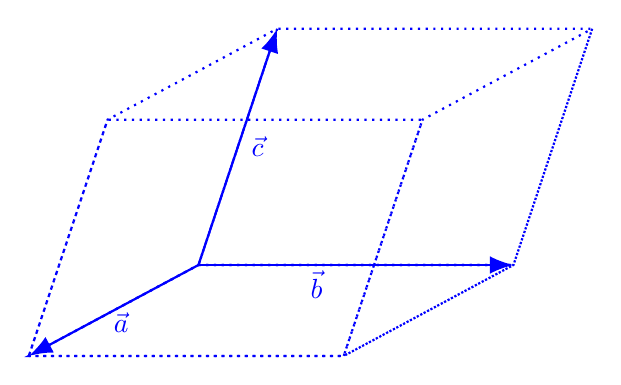
\begin{tikzpicture}%[rotate around y=-15, rotate around z=7]
        % [tdplot_main_coords]
        % Vectors
        % \node[red] at (0, 0, 3.5) {$x$};
        % \node[red] at (3.5, 0, 0) {$y$};
        % \node[red] at (0, 3.5, 0) {$z$};

        % \draw [-{Latex[length=3mm]}, red, thick] (0,0,0) -- (3,0,0);
        % \draw [-{Latex[length=3mm]}, red, thick] (0,0,0) -- (0,3,0);
        % \draw [-{Latex[length=3mm]}, red, thick] (0,0,0) -- (0,0,3);

        \draw [dotted, blue, thick] (0,0,0) -- (4,0,0) -- (3,0,3) -- (-1,0,3) -- cycle;
        \draw [dotted, blue, thick] (0,0,0) -- (4,0,0) -- (5,3,0) -- (1,3,0) -- cycle;
        \draw [dotted, blue, thick] (-1,0,3) -- (3,0,3) -- (4,3,3) -- (0,3,3) -- cycle;
        \draw [dotted, blue, thick] (1,3,0) --(0,0,0) -- (-1,0,3) -- (0,3,3) -- cycle;
        \draw [dotted,blue, thick] (5,3,0) --(4,0,0) -- (3,0,3) -- (4,3,3) -- cycle;
        \draw [-{Latex[length=3mm]}, blue, thick] (0,0,0) -- (-1,0,3);
        \node[blue] at (-0.5,-0.25,1.25) {$\vec{a}$};
        \draw [-{Latex[length=3mm]}, blue, thick] (0,0,0) -- (4,0,0);
        \node[blue] at (1.5,-0.25,0) {$\vec{b}$};
        \draw [-{Latex[length=3mm]}, blue, thick] (0,0,0) -- (1,3,0);
        \node[blue] at (0.75,1.5,0) {$\vec{c}$};
      \end{tikzpicture}
    }
  \end{center}

  \begin{itemize}
  \item Define the oriented volume of $P\vec{a},\vec{b},\vec{c})$ to be
    \[
      V(\vec{a},\vec{b},\vec{c}),
    \]
    where
    \begin{itemize}
    \item $V(e_1,e_2,e_3) = 1$
    \item $|V(\vec{a},\vec{b},\vec{c})|$ is the volume of $P(\vec{a},\vec{b},\vec{c})$
    \item $V$ is an antisymmetric multilinear function
    \end{itemize}
  \end{itemize}
\end{frame}

\begin{frame}
  {Oriented Volume is the Determinant of a $3$-by-$3$ Matrix}

  \begin{itemize}
  \item Suppose $v_1, v_2, v_3 \in V$, where, using Einstein notation,
    \begin{align*}
      \begin{bmatrix} v_1 & v_2 & v_3 \end{bmatrix}
      &= \begin{bmatrix} e_kA^k_1 & e_kA^k_2 & e_kA^k_3 \end{bmatrix}\\
                          &=  \begin{bmatrix} e_1 & e_2 & e_3 \end{bmatrix}
                            \begin{bmatrix} A^1_1 & A^1_2 & A^1_3 \\ A^2_1 & A^2_2 & A^2_3 \\ A^3_1 & A^3_2 & A^3_3 \end{bmatrix}\\
                          &= EA
    \end{align*}
  \item The determinant of $A$ is defined by the equation
    \[
      V(v_1,v_2,v_3) = E\det A
    \]
  \item In particular, since $V(e_1,e_2,e_2) = 1$,
    \[
      \det I = 1
    \]
  \end{itemize}
  
\end{frame}

\begin{frame}
  {Permutations}

  \begin{itemize}
  \item A permutation is a bijective map $\sigma: \{1, \dots, n\} \rightarrow \{1, \dots, n\}$
  \item Let $S_n$ be the set of all permutations of order $n$
  \item A transposition is a permutation $\tau$ that switches two elements and leaves the others unchanged.
    \begin{itemize}
    \item Example: $\tau: \{1, 2, 3, 4\} \rightarrow \{1, 2, 3, 4\}$, where
      \[
        \tau(1) = 1,\ \tau(2) = 4,\ \tau(3) = 3,\ \tau(4)=2
      \]
    \end{itemize}
  \item Every permutation is a composition of transpositions
    \begin{itemize}
    \item Example: The permutation $\sigma(1)=2,\ \sigma(2)=3,\ \sigma(3)=1$ can be written as
      \[
        \sigma = \tau_1\circ\tau_2\text{, where}
      \]
      \begin{align*}
        \tau_1(1)=2,\ \tau_2(2)=1,\ \tau_2(3) &= 3\\
        \tau_2(1)=1,\ \tau_1(2)=3,\ \tau_1(3)=2
      \end{align*}
    \end{itemize}
  \end{itemize}
\end{frame}

\begin{frame}
  {Parity or Sign of a Permutation}

  \begin{itemize}
  \item Given any permutation $\sigma \in S_n$, its parity or sign, which we will write as $\epsilon(\sigma)$, is defined to be
    \begin{itemize}
    \item $1$ if $\sigma$ is the composition of an even number of transpositions
    \item $-1$ if $\sigma$  is the composition of an odd number of transpositions
    \end{itemize}
  \item Easy consequences
    \begin{itemize}
    \item If $\sigma \in S_n$ is a transposition, then $\epsilon(\sigma) = -1$
    \item For any $\sigma, \tau \in S_n$, $\epsilon(\sigma\circ\tau) = \epsilon(\sigma)\epsilon(\tau)$
    \item If $\sigma$ is the identity map, then $\epsilon(\sigma) = 1$
    \item For any $\sigma \in S_n$, $\epsilon(\sigma^{-1}) = \epsilon(\sigma)$ because
      \[
        \sigma = \tau_1\circ\cdots \circ \tau_N \implies \sigma^{-1} = \tau_N\circ\cdots \circ \tau_1
      \]
    \end{itemize}
  \end{itemize}
\end{frame}

\begin{frame}
  {Existence of Sign Function}

  \begin{itemize}
  \item We have stated the properties that the sign function
    \[ \epsilon: S_n \rightarrow \{-1,1\} \]
  \item Claim: There exists a unique function satisfying these properties
  \item This is the consequence of the following:
    \begin{itemize}
    \item A permutation is never both the composition of an even number of transpositions and the composition of an odd number of transpositions
    \end{itemize}
  \item There are straightforward elementary proofs of this
  \item There are also \href{https://mathoverflow.net/questions/417690/conceptual-reason-why-the-sign-of-a-permutation-is-well-defined}{many sophisticated proofs}
  \end{itemize}
\end{frame}

\begin{frame}
  {Automorphisms of $\{1, \dots, n\}$}

  \begin{itemize}
  \item Let $\End(n)$ denote the space of all maps
    \[
      \phi: \{1, \dots, n\} \rightarrow \{1, \dots, n\}
    \]
  \item Observe that $S_n \subset \End(n)$
  \item We can extend the function $\epsilon: S_n \rightarrow \{-1,1\}$ to a function
    \[
      \epsilon: \End(n) \rightarrow \{-1,0,1\},
    \]
    where, if $\phi \in S_n$, then $\epsilon(\phi)$ is as defined before and
    \[
      \epsilon(\phi) = 0\text{ if }\phi \notin S_n
    \]
  \end{itemize}
\end{frame}

\begin{frame}
  {Alternating Multilinear Function on Permutation of Basis}

  \begin{itemize}
  \item Suppose $T: V\times\cdots V \rightarrow \F$ is an alternating multilinear function with $n$ inputs on an $n$-dimensional vector space
  \item Let $(e_1, \dots, e_n)$ be a basis of $V$
  \item If $\phi \in S_n$ is a transposition, then
    \[ T(e_{\phi(1)}, \dots, e_{\phi(n)}) = -T(e_1, \dots, e_n) \]
  \item If $\phi_1,\phi_2 \in S_n$, then
    \begin{multline*}
      T(e_{\phi_2\circ\phi_1(1)}, \dots, e_{\phi_2\circ\phi_1(n)})\\
      = T(e_{\phi_2(1)}, \dots, e_{\phi_2(n)})T(e_{\phi_1(1)}, \dots, e_{\phi_1(n)})
    \end{multline*}
  \item Therefore, for any $\phi \in S_n$,
    \[ T(e_{\phi(1)}, \dots, e_{\phi(n)}) = \epsilon(\phi)T(e_1, \dots, e_n) = \epsilon(\phi)a \]
  \item If $\phi\in \End(n)\backslash S_n$, then it is not injective and therefore
    \[ T(e_{\phi(1)}, \dots, e_{\phi(n)}) = 0 = \epsilon(\phi)T(e_1, \dots, e_n) \]
  \end{itemize}
\end{frame}

\begin{frame}
  {Alternating Multilinear Function With Respect to Basis}

  \begin{itemize}
  \item If $(e_1, e_2, \dots, e_n)$ is a basis of $V$ and $v_k = e_j{\color{blue}a^j_k},\ 1 \le k \le n$,
    \begin{align*}
      T(v_1, \dots, v_n) &= T(e_{j_1}{\color{blue}a^{j_1}_1}, \dots, e_{j_n}{\color{blue}a^{j_n}_n})\\
                         &= \sum_{j_1=1}^n\cdots\sum_{j_n=1}^n T(e_{j_1}, \cdots, e_{j_n}){\color{blue}a_1^{j_1}\cdots a_n^{j_n}}\\
                         &= \sum_{\color{red}{\phi\in\End(n)}} T(e_{\phi(1)}, \cdots, e_{\phi(n)}){\color{blue}a_1^{\phi(1)}\cdots a_n^{\phi(n)}}\\
                         &= \sum_{\color{red}{\phi\in\End(n)}} \epsilon(\phi)T(e_1, \cdots, e_n){\color{blue}a_1^{\phi(1)}\cdots a_n^{\phi(n)}}\\
                         &= T(e_1, \dots, e_n)\sum_{\color{red}{\phi\in \End(n)}}\epsilon(\phi) \color{blue}{a^1_{\phi(1)}\cdots a^n_{\phi(n)}}\\
                         &= T(e_1, \dots, e_n)\sum_{\color{red}{\phi\in S_n}}\epsilon(\phi) \color{blue}{a^1_{\phi(1)}\cdots a^n_{\phi(n)}}
    \end{align*}
  \end{itemize}
\end{frame}

\begin{frame}
  {Space of Alternating Multilinear Functions}

  \begin{itemize}
  \item Let $V$ be an $n$-dimensional vector space
  \item Let $\Lambda^nV^*$ denote the space of antisymmetric alternating functions with $n$ inputs
  \item If $(e_1, \dots, e_n)$ is a basis, then $T \in \Lambda^nV^*$, then $T$ is uniquely determined by the value of
    \[
      T(e_1, \dots, e_n)
    \]
  \item If $T \in \Lambda^nV^*$ is nonzero, then for any $S \in \Lambda^nV^*$, there exists a constant $c \in \F$ such that
    \[
      S = cT
    \]
  \item Specifically,
    \[
      S = \left(\frac{S(e_1, \dots, e_n)}{T(e_1, \dots, e_n)}\right)T
    \]
  \item $\Lambda^nV^*$ is a $1$-dimensional vector space
  \end{itemize}
\end{frame}

\begin{frame}
  {Determinant of an $n$-by-$n$ Matrix}

  \begin{itemize}
  \item Let $(e_1, \dots, e_n)$ be the standard basis of $\F^n$
  \item There is a unique antisymmetric multilinear function
    \[ D: \F^n \times\cdots \times \F^n \rightarrow \F \]
    with $n$ inputs such that
    \[ D(e_1, \dots, e_n) = 1, \]
  \item The formula for $D$ is
    \begin{align*}
      D(v_1, \dots, v_n) &=\sum_{\phi\in\End(n)} b^1_{\phi(1)}\cdots b^n_{\phi(n)}
                           = \sum_{\sigma\in S_n} b^1_{\sigma(1)}\cdots b^n_{\sigma(n)}
    \end{align*}
    where each $v_k = (b_k^1, \dots, b_k^n) = e_jb^j_k$
  \item Let $M$ be an $n$-by-$n$ matrix with columns $C_1, \dots, C_n$
  \item The determinant of $M$ is defined to be
    \[
      \det M = D(C_1, \dots, C_n)
    \]
  \end{itemize}
\end{frame}

\begin{frame}
  {Determinant of an $n$-by-$n$ Matrix}

  \begin{itemize}
  \item The determinant function $det: M_{n\times n} \rightarrow \F$ is the unique function such that
    \begin{itemize}
    \item $\det M$ is an alternating multilinear function of the columns of $M$
    \item $\det I = 1$
    \end{itemize}
  \item If
    \[
      M = \begin{bmatrix} M^1_1 & \cdots & M^1_n \\ \vdots & & \vdots \\ M^n_1 & \cdots & M^n_n \end{bmatrix},\]
    then
    \[
      \det M = \sum_{\phi\in\End(n)}\epsilon(\phi)M^1_{\phi(1)}\cdots M^n_{\phi(n)} = \sum_{\sigma\in S_n}\epsilon(\sigma)M^1_{\sigma(1)}\cdots M^n_{\sigma(n)}
    \]
  \item This formula can be useful in proofs
  \item To calculate the determinant of a specific matrix $M$, it is usually easier to use the properties of an alternating multilinear function
  \end{itemize}
\end{frame}

\begin{frame}
  {Multiplicative Property of the Determinant}

  A fundamental property of the determinant is that if $A$ and $B$ are $n$-by-$n$ matrices, then
  \[
    \det AB = (\det A)(\det B)
  \]
\end{frame}

\begin{frame}
  {Proof of Multiplicative Property}
  
  \begin{itemize}
  \item Given a matrix $A$, define the function $D_A: \F^n\times\cdots\times\F^n \rightarrow \F$ to be
    \[
      D_A(v_1, \dots, v_n) = \det AM,
    \]
    where $(v_1, \dots, v_n)$ are the columns of M
  \item If $C_1, \dots, C_N$ are the columns of $B$, then the $k$-th column of $AB$ is $AC_k$
  \item Therefore,
    \[
      D_A(C_1, \dots, C_n) = \det AB = D(AC_1, \dots, AC_n)
    \]
  \item From this it is easy to see that $D_A$ is an antisymmetric multilinear function of the columns of $B$
  \item Therefore,
    \begin{align*}
      D_A(C_1, \dots, C_n) &= D_A(e_1, \dots, e_n))D(C_1, \dots, C_n)\\
                           &= (\det (AI) )(D(B)) = (\det A)(\det B)
    \end{align*}
  \end{itemize}
\end{frame}


\begin{frame}
  {Transpose of a Matrix}

  \begin{itemize}
  \item Given a matrix $M \in \gl(n,m,\F)$, its transpose is the matrix $M^T \in \gl(m,n,\F)$ that switches the rows and columns
  \item In other words,
    \[
      (M^T)^j_k = M^k_j
    \]
  \item Or
    \[
      \begin{bmatrix} M^1_1 & \cdots & M^1_m \\ \vdots & & \vdots \\ M^n_1 & \cdots & M^n_m \end{bmatrix}^T
      =
      \begin{bmatrix} M^1_1 & \cdots & M^n_1 \\ \vdots & & \vdots \\ M^1_m & \cdots & M^n_m \end{bmatrix}
    \]
  \item If $M \in \mathcal{M}_{n\times m}$, then $M^T \in \gl(m,n,\F)$
  \item For any $A \in \mathcal{M}_{k\times m}$ and $B \in \gl(m,n,\F)$, then $AB \in \mathcal{M}_{k\times n}$ and
    \[
      (AB)^T = B^TA^T \in \mathcal{M}_{n\times k}
    \]
  \end{itemize}
\end{frame}

\begin{frame}
  {Determinant of Matrix Equals Determinant of Its Transpose}

  \begin{itemize}
  \item Lemma: Given any square matrix $M$,
    \[
      \det M^T = \det M
    \]
  \item Proof 1: Use the formula for the determinant
    \begin{align*}
      \det M &= \sum_{\sigma\in S_n}\epsilon(\sigma)M^{\sigma(1)}_1\cdots M^{\sigma(n)}_n\\
             &= \sum_{\sigma\in S_n}\epsilon(\sigma)M^{1}_{\sigma^{-1}(1)}\cdots M^{n}_{\sigma^{-1}(n)}\\
             &= \sum_{\sigma\in S_n}\epsilon(\sigma)M^{1}_{\sigma(1)}\cdots M^{n}_{\sigma(n)}\\
             &= \det M^T
    \end{align*}
  \item Proof 2: Use the following facts to be proved later:
    \begin{itemize}
    \item Any matrix $M$ can be written as $M = PLU$, where
      \begin{itemize}
      \item $P$ is a permutation matrix and $\det P = \det P^T$
      \item $L$ is a lower triangular matrix
      \item $U$ is an upper triangular matrix
      \end{itemize}
    \item Transpose of a triangular matrix is a triangular matrix with same determinant
    \item Transpose of a permutation matrix is a permutation matrix with the same determinant
    \end{itemize}
  \end{itemize}
\end{frame}

\begin{frame}
  {$\det M \ne 0\ \iff M$ is Invertible}

  \begin{itemize}
  \item If the columns of $M$ are linearly dependent, then one column can be written as a linear combination of the others, e.g.,
    \[ C_n = a^1C_1 + \cdots + a^{n-1}C_{n-1}
    \]
  \item It follows that
    \begin{align*}
      \det M &= D(C_1, \dots, C_n)\\
             &= D(C_1, \dots, C_{n-1},a^1C_1 + \cdots + a^{n-1}C_{n-1}\\
             &= a^kD(C_1, \dots, C_{n-1},C_k)\\
             &= 0
    \end{align*}
  \item Recall that $M$ is invertible
    \begin{itemize}
    \item if and only if $\dim \ker M = 0$
    \item if and only if the columns of $M$ are linearly independent
    \end{itemize}
  \item {\bf Conclusion:}
    \begin{itemize}
    \item $M$ is invertible if and only if $\det M \ne 0$
    \item Equivalently, $M$ is singular if and only if $\det M = 0$
    \end{itemize}
  \end{itemize}
\end{frame}

\begin{frame}
  {Determinant of a Linear Transformation}

  \begin{itemize}
  \item Define the determinant of $L$ to be the following: If $E$ is a basis and $L(E) = EM$, then
    \[
      \det(L) = \det(M)
    \]
  \item Given another basis $F$, let $N$ be the matrix such that $L(F) = FN$
  \item Observe that if $F = ET$, where $T$ is an invertible matrix,
    \[
      L(F) = L(ET) = L(E)T = EMT = ET(T^{-1}MT)= F(T^{-1}MT)
    \]
  \item It follows that $N = T^{-1}MT$
  \item Using the basis $N$, the determinant of $L$ is given by
    \begin{align*}
      \det(L) &= \det(N)\\
              &= \det(T^{-1}\det(M)\det(L)\\
              &= \det(M)(\det(T))^{-1}\det(T)\\
              &= \det(M)
    \end{align*}
  \item Therefore, value of $\det(L)$ is independent of the basis used
  \end{itemize}
\end{frame}

\begin{frame}
  {Abstract Definition of $\det(L)$}

  \begin{itemize}
  \item Let $L: V \rightarrow V$ be a linear map
  \item For each $D \in \Lambda^nV^*$, use $L$ to define the following function:
    \[
      L^*D(v_1, \dots, v_n) = D(L(v_1), \dots, L(v_n))
    \]
  \item Using the linearity of $L$, the multilinearity and antisymmmetry of $D$, it is easy to show that $L^*D$ is also an antisymmetric multilinear function.
  \item Therefore, $L^*$ defines a map
    \[
      L^*: \Lambda^nV^* \rightarrow \Lambda^nV^*,
    \]
  \item It is also easy to show that $L^*$ itself is a linear map
  \item Since $\dim(\Lambda^nV^*) = 1$, there is a scalar $d(L)\in \F$, depending on $L$ only such that for any $D \in \Lambda^*V^*$,
    \[
      L^*D = d(L)D
    \]
  \item Define $\det(L)$ to be equal to this scalar $d(L)$
  \end{itemize}
\end{frame}

\begin{frame}
  {Determinant of a Composition}

  \begin{itemize}
  \item If $L_1, L_2$ are linear maps from $V$ to $V$, then
    \begin{align*}
      \det(L_2\circ L_1)D(v_1, \dots, v_n) &= (L_2\circ L_1)^*(D(v_1, \dots, v_n))\\
                                           &= D((L_2\circ L_1)(v_1)), \dots, (L_2\circ L_1)(v_n)))\\
                                           &= D(L_2(L_1(v_1)), \dots, L_2(L_1(v_n)))\\
                                           &= \det(L_2)D(L_1(v_1), \dots, L_1(v_n))\\
                                           &=  \det(L_2)\det(L_1)
    \end{align*}
  \item Since all three definitions of $\det(L)$ are equivalent, this is another proof that
    \[
      \det(M_2M_1) = \det(M_2)\det(M_1)
    \]
  \end{itemize}
\end{frame}

\begin{frame}
  {Eigenvalues and Eigenvectors of a Linear Transformation}

  \begin{itemize}
  \item Consider a linear map $L: V \rightarrow V$
  \item A scalar $\lambda \in \F$ is called an {\bf eigenvalue} of $L$ if there is a nonzero vector $v \in V$ such that any of the following equivalent statements hold
    \[
      L(v) = \lambda v \iff (L-\lambda I)v = 0 \iff v \in \ker (L-\lambda I)
    \]
    The vector $v$ is called an {\bf eigenvector}
  \item $\lambda$ is an eigenvalue of $L$ $\iff$ the linear maps $L - \lambda I$ is singular
  \item Any nonzero $v \in \ker (L-\lambda I)$ is an eigenvector for the eigenvalue $\lambda$
  \item Any nonzero $v \in \ker L$ is an eigenvector for the eigenvalue $0$
  \item The eigenspace for an eigenvalue $\lambda$ of $L$ is the subspace
    \[
      E_\lambda(L) = \ker (L-\lambda I) = \{ v \in V\ :\ L(v) = \lambda v \}
    \]
    A nonzero vector $v$ is an eigenvector for the eigenvalue $\lambda$ if and only if $v \in E_\lambda(L)$
  \end{itemize}
\end{frame}

\begin{frame}
  {Eigenvalues and Eigenvectors of a Square Matrix}

  \begin{itemize}
  \item A scalar $\lambda$ is an {\bf eigenvalue} of a matrix $M \in M_{n\times n}$ if there is a nonzero vector $v \in \F^n$ such that
    \[
      Mv = \lambda v
    \]
    The vector $v$ is called an {\bf eigenvector} for the eigenvalue $\lambda$
  \item If $v$ is an eigenvector for $\lambda$, then so is any nonzero scalar multiple of it
  \item $\lambda$ is an eigenvalue of $M$ if and only if the matrix $M - \lambda I$ is singular
  \item Therefore,
    \[
      \lambda\text{ is an eigenvalue of }M\ \iff\ \det (M-\lambda I) = 0
    \]
  \item $\ker(M-\lambda I)\backslash\{0\}$ is the set of all eigenvectors for the eigenvalue $\lambda$
  \end{itemize}
\end{frame}

\begin{frame}
  {Determinants, Eigenvalues, and Eigenvectors of Similar Matrices}

  \begin{itemize}
  \item Two matrices $M$ and $N$ are called {\bf similar} if there is an invertible matrix $H$ such that
    \[
      M = HNH^{-1}
    \]
    or, equivalently, there is an invertible matrix $G$ such that
    \[
      N = GMG^{-1}
    \]
  \item If $M$ and $N$ are similar, then $\det M = \det N$
  \item $M$ and $N$ have the same eigenvalues, because 
    \[
      Mv = \lambda v\ \iff\ HNH^{-1}v = \lambda v\ \iff\ N(H^{-1}v) = \lambda (H^{-1}v)
    \]
  \end{itemize}
\end{frame}

\begin{frame}
  {Characteristic Polynomial of a Matrix}

  \begin{itemize}
  \item Let $\delta^j_k$ be the element in the $j$-th row and $k$-column of the identity matrix, i.e.,
    \[
      \delta^j_k =
      \begin{cases}
        1 &\text{ if }j=k\\
        0 &\text{ if }j\ne k
      \end{cases}
    \]
  \item Observe that the function $p_M: \F \rightarrow \F$ given by
    \begin{align*}
      p_M(\lambda) &= \det (M-\lambda I)\\
                   &= \sum_{\sigma\in S_n} \epsilon(\sigma)(M-\lambda I)^{\sigma(1)}_1\cdots (M-\lambda I)^{\sigma(n)}_n\\
                   &= \sum_{\sigma\in S_n} \epsilon(\sigma)(M^{\sigma(1)}_1-\lambda \delta^{\sigma(1)}_1)\cdots (M^{\sigma(n)}_n-\lambda \delta^{\sigma(n)}_n)
    \end{align*}
    is a polynomial in $\lambda$ of degree $n$
  \item The roots of $p_M$ are eigenvalues of $M$
  \end{itemize}
\end{frame}

\begin{frame}
  {Similar Matrices Have the Same Characteristic Polynomial}

  \begin{itemize}
  \item If $M = HNH^{-1}$, then
    \[
      M - \lambda I = HNH^{-1} - \lambda H(I)H^{-1} = H(N-\lambda I)H^{-1}
    \]
  \item Therefore,
    \begin{align*}
      p_M(\lambda) &= \det (M-\lambda I)\\
                   &= (\det H)(\det (N-\lambda I))(\det H^{-1})\\
                   &= \det (N-\lambda I)\\
                   &= p_N(\lambda)
    \end{align*}
  \item This is another proof that the eigenvalues of $M$ are the same as the eigenvalues of $N$
  \end{itemize}
\end{frame}

\begin{frame}
  {Eigenvalues of Linear Transformation and its Matrix}

  \begin{itemize}
  \item Consider a linear transformation $L: V \rightarrow V$ on an $n$-dimensional vector space $V$
  \item Given a basis $E = (e_1, \dots, e_n)$ of $V$, there is a matrix $M \in M_{n\times n}$ such that for any $v = Ea$,
    \[
      L(v) = L(Ea) = E(Ma)
    \]
  \item Observe that for any $v \in V$,
    \begin{align*}
      L(v) = \lambda v &\iff L(Ea) = \lambda Ea\\
                       &\iff\ E(Ma) = E(\lambda a)
                       &\iff Ma = \lambda a
    \end{align*}
  \item Therefore, $\lambda$ is an eigenvalue of $L$ iff it is an eigenvalue of $M$
  \end{itemize}
\end{frame}

\begin{frame}
  {Change of Basis formula for a Linear Transformation}
  \begin{itemize}
  \item If $F$ is another basis of $V$, then there is an invertible square matrix $H$ such that $F = EH$
  \item If $v = Ea = Fb$, then
    \[
      v = Fb = EHb,
    \]
    which implies that $a = Hb$ and $b = H^{-1}a$
  \item If $L: V \rightarrow V$ is a linear transformation, then there are matrices $M$ and $N$ such that
    \[
      L(Ea) = E(Ma)\text{ and }L(Fb) = F(Nb) = EHNH^{-1}a,
    \]
    which implies that $M = HNH^{-1}$ and $N = H^{-1}MH$
  \item In other words, $M$ and $N$ are similar and therefore have the same characteristic polynomial
  \end{itemize}
\end{frame}

\begin{frame}
  {Characteristic Polynomial of a Linear Transformation}
  \begin{itemize}
  \item It follows that
    \[
      p_M(\lambda) = \det (M-\lambda I) = \det (N-\lambda I) = p_N(\lambda)
    \]
  \item We can therefore define the characteristic polynomial $p_L$ of a linear transformation $L: V\rightarrow V$ to be
    \[
      p_L = p_M,
    \]
    where $p_M$ is the characteristic polynomial of the matrix $M$ associated to $L$ and a basis of $V$
  \item The polynomial is the same, no matter what basis of $V$ is used
  \end{itemize}
\end{frame}

\begin{frame}
  {Examples}

  \begin{itemize}
  \item Let
    \[
      Z = \begin{bmatrix} 0 & 0 \\ 0 & 0\end{bmatrix},
    \]
  \item $Zv = 0v$ for any $v\in\R^2$ and therefore $0$ is the only eigenvalue
  \item Any nonzero vector $v \in \R^2$ is an eigenvector
  \item The characteristic polynomial is
    \[
      p_Z(x) = \det(Z-\lambda I) = \det\left(\begin{bmatrix} 0 & 0 \\ 0 & 0\end{bmatrix}-
        \lambda\begin{bmatrix} 1 & 0 \\ 0 & 1\end{bmatrix}\right)
      = -\lambda^2
    \]
  \end{itemize}
\end{frame}

\begin{frame}
  {Examples}

  \begin{itemize}
  \item If $D = \begin{bmatrix} a & 0 \\ 0 & b\end{bmatrix} $, then
    $D\begin{bmatrix} v^1\\v^2\end{bmatrix} = \begin{bmatrix} a & 0 \\ 0 & b\end{bmatrix}\begin{bmatrix} v^1\\v^2\end{bmatrix}=\begin{bmatrix} av^1 \\ bv^2 \end{bmatrix}$
  \item If $\lambda = a = b$, then the only eigenvalue is $\lambda$
    \begin{itemize}
    \item Every $v \in \R^2$ is an eigenvector
    \end{itemize}
  \item If $a \ne b$, then the only eigenvalues are $a$ and $b$
    \begin{itemize}
    \item The eigenvectors for the eigenvalue $a$ are
      \[
        \begin{bmatrix} x \\ 0 \end{bmatrix} = x\begin{bmatrix} 1 \\ 0 \end{bmatrix},\ x \in \F\backslash\{0\}
      \]
    \item The eigenvectors for the eigenvalue $b$ are
      \[
        \begin{bmatrix} 0 \\ x \end{bmatrix} = x\begin{bmatrix} 0 \\ 1 \end{bmatrix},\ x \in \F\backslash\{0\}
      \]
    \end{itemize}
  \item The characteristic polynomial is
    \[
      p_D(x) = \det(D-\lambda I)
      = \lambda\begin{bmatrix} a - \lambda & 0 \\ 0 & b-\lambda \end{bmatrix}
      = (a-\lambda)(b-\lambda)
    \]
  \end{itemize}
\end{frame}

\begin{frame}
  {Examples}

  \begin{itemize}
  \item If $A = \begin{bmatrix} 0 & 1 \\ 1 & 0\end{bmatrix}$, then
    $A\begin{bmatrix} v^1\\v^2\end{bmatrix} =\begin{bmatrix} 0 & 1 \\ 1 & 0\end{bmatrix}\begin{bmatrix} v^1\\v^2\end{bmatrix} = \begin{bmatrix} v^2 \\ v^1 \end{bmatrix}$
  \item The only eigenvalues are $1, -1$
  \item The eigenvectors for the eigenvalue $1$ are
    \[ \begin{bmatrix} x \\ x \end{bmatrix},\ x \in \F\backslash\{0\} \]
  \item The eigenvectors for the eigenvalue $-1$ are
    \[ \begin{bmatrix} x \\ -x \end{bmatrix},\ x \in \F\backslash\{0\} \]
  \item The characteristic polynomial is
    \begin{align*}
      p_A(x)
      &= \det\left(\begin{bmatrix} 0 & 1 \\ 1 & 0\end{bmatrix}-\lambda\begin{bmatrix} 1 & 0 \\ 0 & \lambda\end{bmatrix}\right)
        = \det\left(\begin{bmatrix} -\lambda & 1 \\ 1 & \lambda\end{bmatrix}\right)
        = 1-\lambda^2
    \end{align*}
  \end{itemize}
\end{frame}

\begin{frame}{Examples}

  \begin{itemize}
  \item If $B = \begin{bmatrix} 0 & -1 \\ 1 & 0\end{bmatrix}$, then
    $B\begin{bmatrix} v^1\\v^2\end{bmatrix} =\begin{bmatrix} 0 & -1 \\ 1 & 0\end{bmatrix}\begin{bmatrix} v^1\\v^2\end{bmatrix} =\begin{bmatrix} -v^2 \\ v^1 \end{bmatrix}$
  \item There are no real eigenvalues
  \item The complex eigenvalues are $i, -i$
  \item The eigenvectors for the eigenvalue $i$ are
    \[ \begin{bmatrix} ix \\ -x \end{bmatrix} = x\begin{bmatrix} i \\ 1 \end{bmatrix},\ x \in \F\backslash\{0\} \]
  \item The eigenvectors for the eigenvalue $-i$ are
    \[ \begin{bmatrix} x \\ ix \end{bmatrix} = x\begin{bmatrix} 1 \\ i \end{bmatrix},\ x \in \F\backslash\{0\} \]
  \item The characteristic polynomial is
    \begin{align*}
      p_B(x) &= \det(B-\lambda I)\\
             &= \det\left(\begin{bmatrix} -\lambda & -1 \\ 1 & -\lambda \end{bmatrix}\right)\\
             &= 1 + \lambda^2
    \end{align*}
  \end{itemize}
\end{frame}

\begin{frame}
  {Complex Versus Real Eigenvalues}

  \begin{itemize}
  \item If an $n-by-n$ matrix contains only real entries, it can have anywhere from $0$ to $n$ eigenvalues
  \item A polynomial with complex coefficients
    \[ p(x) = a_0 + a_1x + \cdots a_nx^n, \]
    where $a_n \ne 0$ with complex coefficients can always be factored into $n$ linear factors
    \[
      p(x) = a_n(r_1-x)\cdots(r_n-x)
    \]
  \item A complex matrix $A$ always has anywhere from $1$ to $n$ eigenvalues, where an eigenvalue might appear more than once in the factorization of $p_A$
  \item The {\bf multiplicity} of an eigenvalue $\lambda$ is the number of linear factors equal to $(\lambda-x)$ in $p_A$
  \end{itemize}
\end{frame}

\begin{frame}
  {Examples}

  \begin{itemize}
  \item Let
    $D = \begin{bmatrix} 3 & 0 & 0\\ 0 & -2 & 0\\ 0 & 0 & 3 \end{bmatrix}$
  \item The eigenvalues of $D$ are $-2, 3$
  \item The characteristic polynomial of $D$ is
    \[ p_D(\lambda) = (x-3)(x+2)(x-3) = (x-3)^2(x+2) \]
  \item The eigenvalue $3$ has multiplicity $2$, and the eigenvalue $2$ has multiplicity $1$
  \item The eigenvectors for the eigenvalue $-2$ are
    \[ \begin{bmatrix} 0 \\ x \\ 0 \end{bmatrix}=x\begin{bmatrix} 0 \\ 1 \\ 0 \end{bmatrix},\ x \in \F\backslash\{0\} \]
  \item The eigenvectors for the eigenvalue $3$ are
    \[ \begin{bmatrix} x^1 \\ 0 \\ x^2 \end{bmatrix} = x^1\begin{bmatrix} 1 \\ 0 \\ 0\end{bmatrix} + x^2\begin{bmatrix} 0 \\ 0 \\ 1 \end{bmatrix},\  x \in \F\backslash\{0\} \]
  \end{itemize}
\end{frame}

\begin{frame}
  {Examples}

  \begin{itemize}
  \item Let $M = \begin{bmatrix} 1 & 1 \\ 0 & 1 \end{bmatrix}$
  \item The characteristic polynomial of $M$ is
    \[
      p_M(\lambda) = \det(M-\lambda I) = \det\left(\begin{bmatrix} 1-\lambda & 1 \\ 0 & 1-\lambda \end{bmatrix}\right)
      = (1-\lambda)^2
    \]
  \item The only eigenvalue is $1$ with multiplicity $2$
  \item Since
    \[ M\begin{bmatrix} v^1 \\ v^2 \end{bmatrix} = M = \begin{bmatrix} 1 & 1 \\ 0 & 1 \end{bmatrix}\begin{bmatrix} v^1 \\ v^2 \end{bmatrix}
      = \begin{bmatrix} v^1 \\ v^1 + v^2 \end{bmatrix},
    \]
    the eigenvectors of the eigenvalue $1$ are
    \[
      \begin{bmatrix} 0 \\ x \end{bmatrix} = x\begin{bmatrix} 0 \\ 1 \end{bmatrix}
    \]
  \end{itemize}
\end{frame}

\begin{frame}
  {Diagonal Matrices}

  \begin{itemize}
  \item An $n$-by-$n$ matrix $M$ is {\bf diagonal} if
    \[ M^j_k = 0\text{ if }j \ne k \]
  \item In particular, the $k$-th column of $M$ is
    \[ C_k = Me_k = M^k_ke_k\text{ (no sum over $k$),} \]
    where $(e_1, \dots, e_n)$ is the standard basis of $\R^n$
  \item The determinant of $M$ is, by multilinearity,
    \begin{align*}
      D(C_1, \dots, C_n) &= D(M^1_1e_1, M^2_2e_2, \dots, M^n_ne_n)\\ &= D(e_1, \dots, e_n)\\ &= (M^1_1\cdots M^n_n)
    \end{align*}
  \item Since $M-\lambda I$ is also diagonal, it follows that the characteristic polynomial of $M$ is
    \[
      p_M(\lambda) = \det(M-\lambda I) = (M^1_1-\lambda)\cdots(M^n_n-\lambda)
    \]
  \item The diagonal elements of $M$ are its eigenvalues
  \end{itemize}
\end{frame}

\begin{frame}
  {Triangular Matrices}

  \begin{itemize}
  \item An $n$-by-$n$ matrix $M$ is {\bf upper triangular} if it is of the form
    \[ M = \begin{bmatrix} M^1_1 & M^1_2 & \cdots & M^1_{n-1} & M^1_n \\ 0 & M^2_2 & \cdots & M^2_{n-1} & M^2_n \\ \vdots & \vdots & \vdots & \vdots & \vdots \\ 0 & 0 & \cdots & M^{n-1}_{n-1} & M^{n-1}_n \\ 0 & 0 & \cdots & 0 & M^n_n \end{bmatrix} \]
  \item I.e., $M^j_k = 0$ if $j > k$
  \item An $n$-by-$n$ matrix $M$ is {\bf lower triangular} if it is of the form
    \[ M = \begin{bmatrix} M^1_1 & 0 & \cdots & 0  & 0 \\ M^2_1 & M^2_2 & \cdots & 0 & 0 \\ \vdots & \vdots & \vdots & \vdots & \vdots \\ M^{n-1}_1 & M^{n-1}_2  & \cdots & M^{n-1}_{n-1} & 0 \\ M^n_1 & M^n_2 & \cdots & M^n_{n-1} & M^n_n \end{bmatrix} \]
  \item I.e., $M^j_k = 0$ if $j < k$
  \end{itemize}
\end{frame}

\begin{frame}
  {Columns of an Upper Triangular Matrix}

  \begin{itemize}
  \item Let $M$ be an upper triangular matrix and consider the matrix $T = M - \lambda I$
  \item $T$ is itself an upper triangular matrix
  \item Choose a value of $\lambda \in \F$ such that every element on the diagonal of $T$ is nonzero
  \item Let $(e_1, \dots, e_n)$ be the standard basis of $\R^n$
  \item Let $(C_1, \dots, C_n)$ be the columns of $T$
  \item By assumption, $C^1_1, C^2_2, \cdots, C^n_n$ are all nonzero
  \end{itemize}
\end{frame}

\begin{frame}
  {Columns of Upper Triangular Matrix (Part 2)}

  \begin{itemize}
  \item Each column can therefore be written as
    \[
      C_k = C^k_k\hat{C}_k,
    \]
    where
    \[  \hat{C}_k = \begin{bmatrix} \hat{C}^1_k \\ \vdots \\ \hat{C}^{k-1}_k \\ 1 \\ 0 \\ \vdots \\ 0 \end{bmatrix}
      \text{ and }
      \hat{C}^j_k = \frac{C^j_k}{C^k_k}
      \text{, for each }1 \le j, k \le n \]
  \end{itemize}
\end{frame}

\begin{frame}
  {Determinant of Upper Triangular Matrix (Part 1)}

  \begin{itemize}
  \item Let $(C_1, \dots, C_n)$ be the columns of $T$ and recall that the determinant of $T$ is
    \[
      \det(T) = D(C_1, \dots, C_n)
    \]
    where $D \in \Lambda^nV^*$ satisfies $D(e_1, \dots, e_n) = 1$
  \item By the multilinearity of $D$,
    \begin{align*}
      D(C_1, \dots, C_n) &= D(C^1_1\hat{C}_1, C^2_2\hat{C}_2, \dots, C^n_n\hat{C}_n)\\
                         &= (C^1_1C^2_2\cdots C^n_n)D(\hat{C}_1, \dots, \hat{C}_n)
    \end{align*}
  \end{itemize}
\end{frame}

\begin{frame}
  {Determinant of Upper Triangular Matrix (Part 2)}

  \begin{itemize}
  \item Since $T$ is lower triangular, its columns are of the form
    \begin{align*}
      C_1 &= C^1_1e_1\\
      C_2 &= C^1_2e_1 + C^2_2e_2\\
      C_3 &= C^1_3e_1 + C^2_3e_2 + C^3_3e_3\\
      \vdots &\quad \vdots\\
      C_n &= C^1_ne_1 + C^2_ne_2 + C^3_ne_3 + \cdots + C^n_ne_n
    \end{align*}
  \item Similarly,
    \begin{align*}
      \hat{C}_1 &= e_1\\
      \hat{C}_2 &= \hat{C}^1_2e_1 + e_2\\
      \hat{C}_3 &= \hat{C}^1_3e_1 + \hat{C}^2_3e_2 + e_3\\
      \vdots &\quad\quad \vdots\\
      \hat{C}_n &= \hat{C}^1_ne_1 + \hat{C}^2_ne_2 + \hat{C}^3_ne_3 + \cdots + \hat{C}^{n-1}_n e_{n-1} + e_n
    \end{align*}
  \end{itemize}
\end{frame}

\begin{frame}
  {Determinant of Upper Triangular Matrix (Part 3)}

  \begin{itemize}
  \item Therefore,
    \begin{align*}
      \lefteqn{D(\hat{C}_1, \dots, \hat{C}_n)}\\
      &= D(e_1, \hat{C}_2, \dots, \hat{C}_n)\\
      &= D(e_1, \hat{C}^1_2e_1 + e_2, \hat{C}^1_3e_1+\hat{C}^2_3e_2+e_3, \dots, \hat{C}^1e_1 + \cdots + e_n)\\
      &= D(e_1, e_2, \hat{C}^2_3e_2 + e_3, \dots, \hat{C}^2_ne_2 +\cdots+ e_n)\\
      &= D(e_1, e_2, e_3, \dots, \hat{C}^3_ne_3 + \cdots + \cdots + e_n)\\
      &\vdots\quad\quad\vdots\\
      &= D(e_1, e_2, \dots, e_n)\\
      &= 1
    \end{align*}
  \end{itemize}
\end{frame}

\begin{frame}
  {Characteristic Polynomial and Determinant of $M$}
  \begin{itemize}
  \item It follows that if $\lambda$ is not equal to any of $C^1_1, \cdots, C^n_n$,
    \begin{align*}
      p_M(\lambda)  &=\det(T)\\
                    &= D(C_1, \dots, C_n)\\
                    &= C^1_1C^2_2\cdots C^n_nD(\hat{C}_1, \dots,\hat{C}_n)\\
                    &= C^1_1C^2_2\cdots C^n_n\\
                    &= (M^1_1-\lambda I)\cdots(M^n_n-\lambda I)
    \end{align*}
  \item If follows that the polynomial
    \[
      r(\lambda) = p_M(\lambda)-(M^1_1-\lambda I)\cdots(M^n_n-\lambda I)
    \]
    has infinitely many roots
  \item This implies that $r$ is the zero polynomial
  \item Therefore, the characteristic polynomial of an upper triangular matrix $M$ is
    \[ p_M(\lambda) = (M^1_1-\lambda I)\cdots(M^n_n-\lambda I) \]
  \item In particular, $\det(M)=p_M(0)=M^1_1\cdots M^n_n$
  \end{itemize}
\end{frame}

\begin{frame}
  {Diagonal Linear Transformation}

  \begin{itemize}
  \item Let $\dim V = n$
  \item Let $L: V \rightarrow V$ be a linear transformation
  \item Suppose $L$ has $n$ linearly independent eigenvectors $e_1, \dots, e_n$ with eigenvalues $\lambda_1, \dots,\lambda_n$
  \item Then with respect to the basis $E = (e_1, \dots, e_n)$,
    \[
      L(e_k) = e_k\lambda_k
    \]
  \item Equivalently,
    \[ \begin{bmatrix} L(e_1) & \cdots & L(e_n) \end{bmatrix}
      = \begin{bmatrix} e_1 & \cdots & e_n \end{bmatrix}\begin{bmatrix} \lambda_1 & 0 &\cdots & 0 \\ 0 & \lambda_2 & \cdots & 0 \\ \vdots & \vdots & \ddots & \vdots \\ 0 & 0 & \cdots & \lambda_n \end{bmatrix}
    \]
  \end{itemize}
\end{frame}

\begin{frame}
  {Diagonal Linear Transformation}

  \begin{itemize}
  \item Conversely, suppose $L: V \rightarrow V$ is a linear transformation and $E$ is a basis such that
    \[
      L(E) = ED,
    \]
    where $D$ is a diagonal matrix
  \item Then
    \[ L(e_k) = e_jD^j_k = e_kD^k_k \]
  \item Therefore, $L$ has eigenvalues $D^1_1, \dots, D^n_n$ with eigenvectors $e_1, \dots, e_n$ respectively
  \end{itemize}
\end{frame}

\begin{frame}
  {Diagonalizable Linear Transformation}

  \begin{itemize}
  \item Let $L: V \rightarrow V$ be a diagonal linear transformation
  \item If $E$ is a basis of eigenvectors, then
    \[ L(E) = ED, \]
    where $D$ is a diagonal matrix
  \item Given any basis $F$, there is an invertible matrix $M$ such that
    \[ F = EM \]
    and vice versa
  \item There is a matrix $A$ such that
    \[ L(F) = FA \]
  \item Therefore,
    \[ ED = L(E) = L(FM^{-1}) = L(F)M^{-1} = FAM^{-1} = EMAM^{-1} \]
  \item I.e., $M$ and $D$ are similar
  \end{itemize}
\end{frame}

\begin{frame}
  {Diagonalizable Linear Transformation and Matrix}
  \begin{itemize}
  \item A linear transformation $L: V \rightarrow V$ is {\bf diagonalizable} if any of the following equivalent conditions hold:
    \begin{itemize}
    \item There exists a basis of $V$ consisting of eigenvectors
    \item There exists a basis $E$ such that $L(E) = ED$, where $D$ is a diagonal matrix
    \item Given any basis $F$ and matrix $A$ such that
      \[ L(F) = FA, \]
      $A$ is similar to a diagonal matrix
    \item A matrix $A$ is {\bf diagonalizable} if it is similar to a diagonal matrix
    \end{itemize}
  \end{itemize}
\end{frame}

\begin{frame}
  {Linear Transformation With Distinct Eigenvalues}

  \begin{itemize}
  \item Let $\dim(V) = n$ and $L: V \rightarrow V$ be a linear transformation with $n$ distinct eigenvalues $\lambda_1, \dots, \lambda_n$, i.e.,
    \[ j \ne k \implies \lambda_j \ne \lambda_k \]
  \item Let $v_1, \dots, v_n$ be eigenvectors of $\lambda_1, \dots, \lambda_n$ respectively
  \item Suppose $v_1, \dots, v_{k-1}$ are linearly independent
  \item If $a^1v_1 + \cdots + a^kv_kw  = 0$, then
    \begin{align*}
      0 &= (L-\lambda_kI)(a^1v_1 + \cdots + a^kv_k)\\
        &= a^1(Lv_1)-\lambda_kv_1)+\cdots + a^k(L(v_k)-\lambda_kv_k)\\
        &= a^1(\lambda_1-\lambda_k)v_1 + \cdots + a^k(\lambda_k-\lambda_k)v_k\\
        &= a^1(\lambda_1-\lambda_k)v_1 + \cdots + a^{k-1}(\lambda_{k-1}-\lambda_k)v_{k-1},
    \end{align*}
  \item Therefore, $a^1(\lambda_1-\lambda_k) = \cdots = a^{k-1}(\lambda_{k-1}-\lambda_k) = 0$
  \end{itemize}
\end{frame}

\begin{frame}
  {Linear Transformation With Distinct Eigenvalues}

  \begin{itemize}
  \item Since $v_1, \dots, v_{k-1}$ are linearly independent, it follows that
    \[  a^1(\lambda_1-\lambda_k) = \cdots = a^{k-1}(\lambda_{k-1}-\lambda_k) = 0 \]
  \item Since the eigenvalues are distinct, this implies that
    \[ a^1 = \cdots = a^{k-1} = 0 \]
  \item By assumption, $a^1v_1 + \cdots + a^kv_kw  = 0$ and therefore $a^k = 0$
  \item It follows by induction that $v_1, \dots, v_n$ form a basis of $V$
  \item Therefore, $L$ is diagonalizable
  \item {\bf Conclusion: }Any linear transformation with $n$ distinct eigenvalues is diagonalizable
  \end{itemize}
\end{frame}

\begin{frame}
  {Direct Sum of Subspaces}

  \begin{itemize}
  \item Let $V_1, \dots, V_k$ be subspaces of $V$
  \item $\{ V_1, \dots, V_k \}$ is a {\bf linearly independent} set of subspaces if for any nonzero vectors
    \[ v_1 \in V_1,\ v_2 \in V_2, \dots, v_k \in V_k \]
    are linearly independent
  \item Equivalently, $\{ V_1, \dots, V_k \}$ is linearly independent if for any $v_1 \in V_1,\dots, v_k\in V_k$,
    \[
      v_1 + v_2 + \cdots + v_k = 0 \implies v_1 = v_2 = \cdots = v_k
    \]
  \item Equivalently,  $\{ V_1, \dots, V_k \}$ is linearly independent if for any $v_1,w_1 \in V_1,\dots, v_k,w_k\in V_k$,
    \[
      v_1+v_2+\cdots+v_k=w_1+w_2+\cdots+w_k\implies v_1=w_1, \dots, v_k=w_k
    \]
  \item If $\{V_1, V_2, \dots, V_k\}$ is linearly independent, then their {\bf direct sum} is defined to be
    \[
      V_1\oplus V_2 \oplus \cdots \oplus V_k = \operatorname{span}(V_1\cup V_2\cup\cdots\cup V_k)
    \]
  \end{itemize}
\end{frame}

\begin{frame}
  {Examples}

  \begin{itemize}
  \item $\{S_1, S_2\}$, where $S_1,S_2 \subset \F^3$ are given by
    \begin{align*}
      S_1 &= \operatorname{span}(e_1)\\
      S_2 &= \operatorname{span}(e_2),
    \end{align*}
    is linearly independent
  \item If $\{ v_1, \dots, v_k\}$ is linearly independent and
    \[ \forall 1 \le j \le k,\ V_j = \operatorname{span}(v_j), \]
    then $\{V_1, \dots, V_k\}$ is a linearly independent set of subspaces
  \item If $(e_1,e_2,e_3,e_4)$ is a basis of $V$ and
    \[ S = \operatorname{span}(e_1,e_2,e_3),\ T = \operatorname{span}(e_4), \]
    then $V = S\oplus T$
  \end{itemize}
\end{frame}

\begin{frame}
  {Eigenspaces of Distinct Eigenvalues are Linearly Independent (Part 1)}

  \begin{itemize}
  \item If $\lambda_1, \dots, \lambda_k$ are distinct eigenvalues of $L: V \rightarrow V$, then their eigenspaces $E_{\lambda_1}, \dots, E_{\lambda_k}$ are linearly independent
  \item Prove by induction that for any $1 \le j \le k$,
    \[
      v_1 + \cdots + v_j = 0 \implies v_1=\cdots = v_j = 0
    \]
  \item This holds for $j=1$
  \item Inductive step: Assume that it holds for $1 \le j < k$ and prove it holds for $j+1$
  \end{itemize}
\end{frame}

\begin{frame}
  {Eigenspaces of Distinct Eigenvalues are Linearly Independent (Part 2)}

  \begin{itemize}
  \item Suppose $v_1 \in E_{\lambda_1}, \dots, v_{j+1}\in E_{\lambda_{j+1}}$ satisfy
    \begin{equation}\label{assumption}
      v_1 + \cdots + v_{j+1} = 0
    \end{equation}
  \item It follows that
    \begin{align*}
      0 &= (L-\lambda_{j+1}I)(v_1 + \cdots + v_{j+1})\\
        &= (\lambda_1-\lambda_{j+1})v_1 + \cdots + (\lambda_j-\lambda_{j+1})v_j
    \end{align*}
  \item By the inductive assumption,
    \[ (\lambda_1-\lambda_{j+1})v_1=\cdots=(\lambda_j-\lambda_{j+1})v_j=0 \]
  \item Since $\lambda_i-\lambda_{j+1}\ne 0$ for each $1 \le i \le j$,
    \[ v_1 = \cdots = v_j = 0 \]
  \item By \eqref{assumption}, it follows that $v_{j+1}=0$
  \end{itemize}
\end{frame}

\begin{frame}
  {Eigenspaces of Distinct Eigenvalues are Linearly Independent (Part 3)}

  \begin{itemize}
  \item By induction,
    \[ 
      v_1 + \cdots + v_k = 0 \implies v_1=\cdots = v_k = 0
    \]
  \item This implies that $E_{\lambda_1}, \dots, E_{\lambda_k}$ are linearly independent
  \end{itemize}
\end{frame}

\begin{frame}
  {Diagonalizability of a Linear Transformation (Part 1)}

  \begin{itemize}
  \item Let $\lambda_1, \dots, \lambda_k$ be the eigenvalues of $L: V\rightarrow V$
  \item $L$ is diagonalizable if and only if
    \[ \dim(E_{\lambda_1}) + \cdots + \dim(E_{\lambda_k}) = \dim V \]
  \item Let $n_0 = 0$ and, for $1 \le j \le k$, let
    \begin{align*}
      n_j &= \dim(E_{\lambda_j})\\
      N_j &= n_1 + \cdots + n_{j}
    \end{align*}
  \item For each $1 \le j \le k$, let
    \[
      (v_{N_{j-1}+1}, \cdots, v_{N_j})
    \]
    be a basis of $E_{\lambda_j}$
  \end{itemize}
\end{frame}

\begin{frame}
  {Diagonalizability of a Linear Transformation (Part 2)}

  \begin{itemize}
  \item Suppose
    \[
      a^1v_1 + \cdots + a^nv_n = 0,
    \]
  \item For each $1 \le j \le k$, let
    \[
      w_j = a^{N_{j-1}+1}v_{N_{j-1}}+ \cdots+ a^{N_j}v_{N_j} \in E_{\lambda_j}
    \]
  \item Since $w_1+\cdots+w_k = 0$, it follows that
    \[
      w_1 = \cdots = w_k = 0
    \]
  \item For each $1 \le j \le k$,
    \[ 0 = w_j = a^{N_{j-1}+1}v_{N_{j-1}}+ \cdots+ a^{N_j}v_{N_j}, \]
    which implies $a^{N_{j-1}+1}= \cdots=a^{N_j}=0$
  \item Therefore, $(v_1, \dots, v_n)$ is a basis of $V$
  \item $L$ is diagonal with respect to this basis
  \end{itemize}
\end{frame}

\begin{frame}
  {Dot Product on $\R^n$}

  \begin{itemize}
  \item Recall that the {\bf dot product} of
    \[
      v = \begin{bmatrix} v^1\\ \vdots \\ v^n \end{bmatrix},\ w = \begin{bmatrix} w^1\\ \vdots \\ w^n \end{bmatrix} \in \R^n
    \]
    is defined to be
    \[
      v\cdot w = v^1w^1+\cdots+v^nw^n = v^Tw = w^Tv
    \]
  \item The {\bf norm} or {\bf magnitude} of $v \in \R^n$ is defined to be
    \[
      |v| = \|v\| = \sqrt{v\cdot v}
    \]
  \item If $v$ and $w$ are nonzero and the angle at $0$ from $v$ to $w$ is $\theta$, then
    \[
      \cos\theta = \frac{v\cdot w}{|v||w|}
    \]
  \end{itemize}
\end{frame}

\begin{frame}
  {Properties of Dot Product}

  \begin{itemize}
  \item The dot product is {\bf bilinear} because for any $a,b \in \R$ and $u,v,w \in \R^n$,
    \begin{align*}
      (au+bv)\cdot w &= a(u\cdot w) + b(v\cdot w)\\
      u\cdot(av+bw) &= a(u\cdot v)+b(u\cdot w)
    \end{align*}
  \item It is {\bf symmetric}, because for any $v, w \in \R^n$,
    \[ v\cdot w = w\cdot v \]
  \item It is {\bf positive definite}, because for any $v \in \R^n$,
    \[
      v\cdot v \ge 0
    \]
    and 
    \[
      v\cdot v > 0 \iff v \ne 0
    \]
  \end{itemize}
\end{frame}

\begin{frame}
  {Inner Product on Real Vector Space}

  \begin{itemize}
  \item Let $V$ be an $n$-dimensional real vector space
  \item Consider a function
    \[ \alpha: V\times V \rightarrow \R \]
  \item It is {\bf bilinear} if for any $a, b \in \R$ and $u,v,w\in \R^n$,
    \begin{align*}
      \alpha(au+bv,w) &= a\alpha(u,w) + b\alpha(v,w)\\
      \alpha(u,av+bw) &= a\alpha(u,v) + b\alpha(u,w)
    \end{align*}
  \item It is {\bf symmetric} if for any $v,w \in \R^n$,
    \[ \alpha(v,w) = \alpha(w,v) \]
  \item It is {\bf positive definite} if for any $v \in \R^n$,
    \[
      \alpha(v,v) \ge 0
    \]
    and
    \[
      \alpha(v,v) > 0 \iff v \ne 0
    \]
  \item Any positive definite symmetric bilinear function on a {\bf real} vector space $V$ is called an {\bf inner product}
  \end{itemize}
\end{frame}

\begin{frame}
  {Hermitian Inner Product on $\C^n$}

  \begin{itemize}
  \item Recall that if $z = x+iy \in \C$, then
    \[
      \bar{z} = x-iy\text{ and }z\bar{z} = \bar{z}z = x^2+y^2
    \]
  \item If $A$ is a complex matrix, its {\bf Hermitian adjoint} is defined to be
    \[
      A^* = \bar{A}^*
    \]
  \item The Hermitian inner product on $\C^n$ of
    \[
      v = \begin{bmatrix} v^1\\ \vdots \\ v^n \end{bmatrix},
      \ w = \begin{bmatrix} w^1\\ \vdots \\ w^n \end{bmatrix} \in \C^n
    \]
    is defined to be
    \[
      (v,w) = v^1\bar{w}^1+\cdots+v^n\bar{w}^n = v^T\bar{w} = \bar{w}^Tv = w^*v\in \C,
    \]
  \item The {\bf norm} of $v \in \C^n$ is defined to be
    \[
      |v| = \|v\| = \sqrt{(v,v)}
    \]
  \item {\bf No} geometric interpretation of the Hermitian inner product
  \end{itemize}
\end{frame}

\begin{frame}
  {Not a Real Inner Product}
  \begin{itemize}
  \item {\bf Not} bilinear, because if $c \in \C$,
    \[
      (v,cw) = \bar{c}(v,w)
    \]
  \item {\bf Not} symmetric, because
    \[
      (w,v) = \overline{(v,w)}
    \]
  \item It is positive definite, because for any $v \in \C^n$, $(v,v) \in \R$,
    \[
      (v,v) = v^1\bar{v}^1 + \cdots + v^n\bar{v}^n = |v^1|^2 + \cdots + |v^n|^2 \ge 0,
    \]
    and
    \[
      (v,v) \ne 0 \iff v \ne 0
    \]
  \end{itemize}
\end{frame}

\begin{frame}
  {Properties of Hermitian Inner Product on $\C^n$}

  \begin{itemize}
  \item It is a linear function of the first argument, because for any $a, b \in \C$, $u,v,w\in \C^n$,
    \[
      (au+bv,w) = a(u,w) + b(v,w)
    \]
  \item It is {\bf Hermitian}, which means
    \[ (v,w) = \overline{(w,v)} \]
  \item Therefore, for any $a,b \in \C$ and $u,v,w\in \C^n$,
    \[ (u,av+bw) = \bar{a}(u,v) + \bar{b}(a,w) \]
  \end{itemize}
\end{frame}

\begin{frame}
  {Inner Product of a Vector Space Over $\F$}

  \begin{itemize}
  \item Assume $\F$ is $\R$ or $\C$
  \item An {\bf inner product} over a vector space $V$ is a function
    \begin{align*}
      (\cdot,\cdot): V\times V &\rightarrow \F
    \end{align*}
    with the following properties: For any $a,b \in F$ and $u,v,w\in V$,
    \begin{align*}
      (au+bv,w) &= a(u,w)+b(v,w)\\
      (w,v) &= \overline{(v,w)}\\
      (v,v) &\ge 0\\
      (v,v) &\ne 0 \iff v\ne 0
    \end{align*}
  \item If $\F = \R$, this is the same definition as before
  \item If $\F = \C$, this is the definition of a Hermitian inner product
  \end{itemize}
\end{frame}

\begin{frame}
  {Examples}

  \begin{itemize}
  \item For each $v \in \F^n$, denote $v^* = \bar{v}^T$
  \item The standard inner product on $\F^n$ is
    \[
      (v,w) = w^*v,
    \]
    which is the dot product on $\R^n$ and the standard Hermitian inner product on $\C^n$
  \item An inner product on the space of polynomials of degree $n$ or less and with coefficients in $\F$ is
    \[
      (f,g) = \int_{t=0}^{t=1} f(t)\overline{g(t)}\,dt
    \]
  \item An inner product on the space of matrices with $n$ rows and $m$ columns is
    \[
      (A,B) = \trace(B^*A) = \sum_{1\le k\le m}\sum_{1\le j\le n} \bar{B}^j_kA^j_k,
    \]
    where $B^* = \bar{B}^T$
  \end{itemize}
\end{frame}

\begin{frame}
  {Nondegeneracy Property}

  \begin{itemize}
  \item Fact: If a vector $v \in V$ satisfies the following property:
    \[
      \forall w \in V,\ (v,w) = 0,
    \]
    then $v = 0$
    \begin{itemize}
    \item Proof: Setting $w = v$, it follows that
      \[
        (v,v) = 0\text{ and therefore }v=0
      \]
    \end{itemize}
  \item Corollary: If $v_1, v_2 \in V$ satisfy the property that
    \[
      \forall w\in V,\ (v_1,w) = (v_2,w),
    \]
    then $v_1 = v_2$
  \item Corollary: If $`L_1, L_2: V \rightarrow W$ are linear maps such that
    \[
      \forall v\in V,\ w \in W,\ (L_1(v),w) = (L_2(v),w),
    \]
    then $L_1=L_2$
    \begin{itemize}
    \item Proof: Given $v \in V$,
      \[
        \forall w \in W,\ (L_1(v),w) = (L_2(v),w),
      \]
      which implies $L_1(v)=L_2(v)$
    \item Since this holds for all $v \in V$, it follows that $L_1=L_2$
    \end{itemize}
  \end{itemize}
\end{frame}

\begin{frame}
  {Fundamental Inequalities}

  \begin{itemize}
  \item {\bf Cauchy-Schwarz inequality:} For any $v, w\in V$,
    \[ |(v,w)| \le |v||w| \]
    and
    \[ |(v,w)| = |v||w| \]
    if and only if there exists $s \in \F$ such that
    \begin{align*}
      v &= sw\text{ or }w = sv
    \end{align*}
  \item {\bf Triangle inequality:} For any $v, w\in V$,
    \[ |v+w| \le |v|+|w| \]
    and
    \[ |v+w| = |v|+|w| \]
    if and only if $v = \pm w$
  \end{itemize}
\end{frame}

\begin{frame}
  {Proof When $\F=\R$}
  \begin{itemize}
  \item If $v = 0$ or $w = 0$, equality holds
  \item Let
    \begin{align*}
      f(t) &= |v-tw|^2\\
           &= (v-tw,v-tw)\\
           &= |v|^2 - 2t(v,w) + t^2|w|^2\\
           &= \left(t|w|-\frac{(v,w)}{|w|}\right)^2 + |v|^2-\frac{(v,w)^2}{|w|^2}
    \end{align*}
  \item $f$ has a unique minimum when $t = t_{\min}$, where
    \[
      t_{\min} = \frac{(v,w)}{|w|}\text{ and }f(t_{\min}) = |v|^2-\frac{(v,w)^2}{|w|^2}
    \]
  \end{itemize}
\end{frame}

\begin{frame}
  {Proof of Cauchy-Schwarz (Part 1)}
  \begin{itemize}
  \item If $v = 0$ or $w = 0$, equality holds
  \item If $w \ne 0$, let $f: \F \rightarrow \R$ be the function
    \begin{align*}
      f(t) &= |v-tw|^2\\
           &= (v-tw,v-tw)\\
           &= |v|^2 - t(w,v)-\bar{t}(v,w) + |t|^2|w|^2
    \end{align*}
  \item If $f$ has a minimum at $t_0 \in \F$, then its directional derivative at $t_0$ is zero in any direction $\dot{t}$
    \begin{align*}
      0 &= \left.\frac{d}{ds}\right|_{s=0}f(t_0+s\dot{t})\\
        &= -\dot{t}(w,v)-\overline{\dot{t}}(v,w)+(t_0\overline{\dot{t}}+\bar{t}_0\dot{t})|w|^2\\
        &= \dot{t}(\bar{t}_0-(w,v)) + \overline{\dot{t}}(t_0|w|^2-(v,w))\\
        &= \dot{t}(\overline{t_0-(v,w)}) + \overline{\dot{t}}(t_0|w|^2-(v,w))
    \end{align*}
  \end{itemize}
\end{frame}

\begin{frame}
  {Proof of Cauchy-Schwarz (Part 2)}

  \begin{itemize}
  \item In particular, if
    \[ \dot{t} = t_0|w|^2-(v,w), \]
    we get
    \[
      |t_0|w|^2-(v,w)|^2=0,
    \]
  \item Therefore, the only critical point of $f$ is
    \[
      t_0 = \frac{(v,w)}{|w|^2}
    \]
  \item Since $f$ is always nonnegative, it follows that
    \begin{align*}
      0 &\le f(t_0) = |v|^2 - \frac{|(v,w)|^2}{|w|^2}
    \end{align*}
    which implies the Cauchy-Schwarz inequality
  \end{itemize}
\end{frame}

\begin{frame}
  {Proof of Cauchy-Schwarz (Part 3)}

  \begin{itemize}
  \item If $w \ne 0$ and $|(v,w)| = |v||w|$, then
    \[
      0 = |v|^2-\frac{|(v,w)|^2}{|w|^2} = f(t_0) = |v-t_0w|^2,
    \]
    which implies that
    \[
      v = t_0w
    \]
  \end{itemize}
\end{frame}

\begin{frame}
  {Proof of Triangle Inequality}

  \begin{itemize}
  \item The triangle inequality follows easily from Cauchy-Schwarz inequality
    \begin{align*}
      |v+w|^2 &= (v+w,v+w)\\
              &= |v|^2 + (v,w) + (w,v) + |w|^2\\
              &\le |v|^2 + |(v,w)| + |(w,v)| + |w|^2\\
              &\le |v|^2 + 2|v||w| + |w|^2\\
              &= (|v|+|w|)^2
    \end{align*}
  \item If $|v+w|=|v|+|w|$, then
    \[
      |(v,w)| = |(v,w)| = |v||w|,
    \]
    which implies $v = tw$ and therefore
    \begin{align*}
      |t+1|^2|w|^2 &= |tw+w|^2&= |tw|^2 + |w|^2= (|t|^2+1)|w|^2,
    \end{align*}
    which implies that $t = \bar{t}$, i.e., $t \in \R$
  \end{itemize}
\end{frame}

\begin{frame}
  {Polarization Identities}

  \begin{itemize}
  \item On $\R^n$
    \begin{align*}
      (v,w) &= \frac{1}{4}(|v+w|^2 - |v-w|^2)
    \end{align*}
  \item On $\C^n$
    \begin{align*}
      (v,w) &= \frac{1}{4}(|v+w|^2 + i|v+iw|^2 - |v-w|^2 - i|v-iw|^2)
    \end{align*}
  \end{itemize}
\end{frame}

\begin{frame}
  {Norm Defined by Inner Product}

  \begin{itemize}
  \item The norm of $v \in V$,
    \[ |v| = \sqrt{(v,v)} \]
    satisfies the following properties for any $s \in \F$, $v, w \in V$
    \begin{align*}
      |sv| &= |s||v| &\text{(Homogeneity)}\\
      |v| &\ge 0 &\text{(Nonnegativity)}\\
      |v| &= 0 \iff v = 0 &\text{(Nondegeneracy)}\\
      |v+w| &\le |v|+|w| &\text{(Triangle inequality)}
    \end{align*}
  \item Homogeneity and the triangle inequality imply convexity: For any $0 \le t \le 1$ and $v, w \in V$,
    \begin{align*}
      |(1-t)v+tw| &\le (1-t)|v|+t|w|
    \end{align*}
  \end{itemize}
\end{frame}

\begin{frame}
  {Norm}

  \begin{itemize}
  \item A norm on a vector space $V$ over $\F$ is a function
    \[
      g: V \rightarrow \R,
    \]
    that satisfies for any $s \in \F$ and $v,w\in V$,
    \begin{align*}
      |sv| &= |s||v| &\text{(Homogeneity)}\\
      |v| &\ge 0 &\text{(Nonnegativity)}\\
      |v| &= 0 \iff v = 0 &\text{(Nondegeneracy)}\\
      |v+w| &\le |v|+|w| &\text{(Triangle inequality)}
    \end{align*}
  \end{itemize}
\end{frame}

\begin{frame}
  {Examples of Norms}

  \begin{itemize}
  \item Given $1 \le p < \infty$, the $\ell_p$ norm of $v \in\F^n$ is defined to be
    \[
      |v|_p = (|v^1|^p+\cdots+|v^n|^p)^{1/p}
    \]
  \item The $\ell_\infty$ norm of $v \in\F^n$ is defined to be
    \[
      |v|_\infty = \max(|v^1|, \dots, |v^n|) = \lim_{p\rightarrow\infty}|v|_p
    \]
  \item The $L_p$ norm of a continuous function $f: [0,1]\rightarrow \C$ is defined to be
    \[
      \|f\|_p = \left(\int_{x=0}^{x=1}|f(x)|^p\,dx\right)^{1/p}
    \]
  \item The $L_\infty$ norm of a continuous function $f: [0,1] \rightarrow \C$ is defined to be
    \[
      \|f\|_\infty = \sup \{ |f(x)|\ :\ 0 \le x \le 1 \} = \lim_{p\rightarrow\infty}\|f\|_p
    \]
  \end{itemize}
\end{frame}

\begin{frame}
  {Parallelogram Identity}

  \begin{itemize}
  \item A norm $|\cdot|$ on a vector space $V$ satisfies the parallelogram identity
    \[
      |v+w|^2 + |v-w|^2 = 2(|v|^2+|w|^2),\ \forall v, w \in V
    \]
    if and only if there is an inner product on $V$ such that
    \[
      |v|^2 = (v,v)
    \]
  \end{itemize}
\end{frame}

\begin{frame}
  {Orthogonality For Standard Dot Product on $\R^n$}

  \begin{itemize}
  \item The following are synonyms: orthogonal, perpendicular, normal
  \item On $\R^n$,
    \begin{itemize}
    \item Two vectors $v_1, v_2$ are called {\bf orthogonal} if
      \[
        v_1\cdot v_2 = 0
      \]
    \item A basis $(v_1, \dots, v_n)$ is called {\bf orthonormal} if for any $1 \le i, j \le n$,
      \[
        v_i\cdot v_j = \delta_{ij} =
        \begin{cases} 1 &\text{ if }i=j\\
          0 &\text{ if }i \ne j
        \end{cases}
      \]
    \end{itemize}
  \end{itemize}
\end{frame}

\begin{frame}
  {Orthogonality on an Inner Product Space}

  \begin{itemize}
  \item Let $V$ be an $n$-dimensional vector space over $\F$ with inner product $(\cdot,\cdot)$
  \item Two vectors $v_1, v_2$ are {\bf orthogonal} if
    \[
      (v_1,v_2) = 0
    \]
  \item Vectors $v_1, \dots, v_k$ are {\bf mutually orthogonal} if for every $1 \le i < j \le k$,
    \[
      (v_i,v_j) \ne 0
    \]
  \item Mutually orthogonal vectors must all be nonzero
  \item A set of muturally orthogonal vectors is called an {\bf orthogonal set}
  \end{itemize}
\end{frame}

\begin{frame}
  {Linear Independence of Orthogonal Set}
  
  \begin{itemize}
  \item An orthogonal set is linearly independent, because if
    \[
      a^1v_1 + \cdots + a^kv_k = 0,
    \]
    then for any $1 \le j \le k$,
    \[
      0 = (v_j,a^1v_1 + \cdots + a^kv_k) = a^j(v_j,v_j)
    \]
    Since $v_j \ne 0$, $(v_j,v_j) \ne 0$ and therefore $a^j = 0$
  \item If
    \[
      v = a^1v_1 + \cdots + a^kv_k,
    \]
    then for each $1 \le j \le k$,
    \[
      a^j = \frac{(v,v_j)}{|v_j|}
    \]
    and
    \[
      v = \frac{(v,v_1)}{|v_1|} + \cdots + \frac{(v,v_k)}{|v_k|}
    \]
  \item Any orthogonal set of $n$ vectors is a basis
  \end{itemize}
\end{frame}

\begin{frame}
  {Orthonormal Set and Basis}

  \begin{itemize}
  \item $\{v_1, \dots, v_k\} \subset V$ is called an {\bf orthonormal} set if for any $1 \le i,j \le k$,
    \[
      (v_i,v_j) = \delta_{ij}
    \]
  \item If $\F = \C$, such a set is also called a {\bf unitary} set
  \item An orthonormal set of $n$ elements is called an {\bf orthonormal} or {\bf unitary} basis
  \item Any orthogonal set $\{ v_1, \dots, v_k \}$ can be turned into an orthonormal set,
    \[
      \{ \frac{v_1}{|v_1}, \dots, \frac{v_k}{|v_k|}
    \]
  \item An orthormal or unitary basis is an orthonormal set with $n$ elements,
    \[
      E = (e_1, \dots, e_n) \subset V
    \]
  \item If $v = a^1e_1 + \dots + a^ne_n$, then
    \[
      a_j = (v,e_j)
    \]
  \item I.e.,
    \[
      v = (v,e_1)e_1 + \cdots + (v,e_n)e_n
    \]
  \end{itemize}
\end{frame}

\begin{frame}
  {Example: Finite Fourier Decomposition (Part 1)}

  \begin{itemize}
  \item For each $-N \le k \le N$, consider
    \begin{align*}
      v_k: [0,2\pi] &\rightarrow \C\\
      \theta &\mapsto e^{ik\theta}
    \end{align*}
  \item Let
    \[
      V = \{ a^{-N}v_N + \cdots + a^0 + \cdots + a^Nv_N\ :\ (a^1, \dots, a^N)\in \C^{2N+1} \}.
    \]
  \item $V$ is a $(2N+1)$-dimensional complex vector space
  \item Consider the inner product
    \[
      (f_1,f_2) = \int_{\theta=0}^{\theta=2\pi} f_1(\theta)\bar{f}_2(\theta)\,d\theta
    \]
  \end{itemize}
\end{frame}

\begin{frame}
  {Finite Fourier Decomposition (Part 2)}

  \begin{itemize}
  \item If $j \ne k$, then
    \begin{align*}
      (v_j,v_k) &= \int_{\theta=0}^{\theta=2\pi} e^{i(j-k)\theta}\,d\theta\\
                &= \left.\frac{e^{i(j-k)\theta}}{i(j-k)}\right|_{\theta=0}^{\theta=2\pi}\\
                &= 0\\
      (v_k,v_k) &= \int_{\theta=0}^{\theta=2\pi} 1\,d\theta\\
                &= 2\pi
    \end{align*}
  \item Therefore, $(v_{-N}, \dots, v_N)$ is an orthogonal basis, and
    $(u_{-N}, \dots, u_N)$, where
    \[ u_k = \frac{v_k}{\sqrt{2\pi}},\ -N \le k \le N, \]
    is an orthonormal basis
  \end{itemize}
\end{frame}

\begin{frame}
  {Finite Fourier Decomposition (Part 3)}

  \begin{itemize}
  \item Given any $f: C^0([0,2\pi])$, let
    \[
      f_N(\theta) = a^{-N}u_{-N} + \cdots + a^Nu_N,
    \]
    where
    \[
      a^k = (f,u_k) = \frac{1}{\sqrt{2\pi}}\int_{\theta=0}^{\theta_2\pi} f(\theta)e^{-ik\theta}\,d\theta
    \]
  \item When is $f_N$ is a good approximation to $f$?
  \item When is
    \[
      f = \sum_{k=-\infty}^{k=\infty} a^ku_k?
    \]
  \end{itemize}
\end{frame}

\begin{frame}
  {Orthogonal Complement}

  \begin{itemize}
  \item Let $V$ be a vector space with inner product $(\cdot,\cdot)$
  \item Given a subspace $E \subset V$, define its {\bf orthogonal complement} to be the subspace
    \[
      E^\perp = \{ v \in V\ :\ \forall e \in E, (v,e) = 0 \}
    \]
  \item $E\cap E^\perp = \{0\}$, because if
    \[ v \in E\cap E^\perp, \]
    then \[ |v|^2 = (v,v) = 0, \]
  \item If $v_1, v_2 \in E$, $w_1,w_2 \in E^\perp$, and
    \[
      v_1+w_1 = v_2+v_2,
    \]
    then
    \[
      v_1-v_2 = w_2-w_1 \in E\cap E^\perp
    \]
    and therefore, $v_1 = v_2$ and $w_1 = w_2$
  \item If follows that $E\oplus E^\perp$ is a subspace of $V$
  \end{itemize}
\end{frame}

\begin{frame}
  {Orthogonal Decomposition}

  \begin{itemize}
  \item For each $v \in E\oplus E$, there exist unique $v_1 \in E$ and $v_2\in E^\perp$ such that
    \[
      v = v_1 + v_2
    \]
  \item Define the orthogonal projection maps
    \begin{align*}
      P_E: E\oplus E^\perp &\rightarrow E\\
      v &\mapsto v_1
    \end{align*}
    and
    \begin{align*}
      P_E^\perp: E\oplus E^\perp &\rightarrow E^\perp\\
      v &\mapsto v_2
    \end{align*}
  \end{itemize}
\end{frame}

\begin{frame}
  {Orthogonal Projection Maps}

  \begin{itemize}
  \item $P_E, P^\perp_E$ are linear maps
  \item $P_E: E\oplus E^\perp \rightarrow E$ is projection onto $E$:
    \begin{align*}
      \forall v \in E,\ P_E(v) &= v\\
    \end{align*}
  \item $P^\perp_E: E\oplus E^\perp \rightarrow E^\perp$ is projection onto $E^\perp$:
    \begin{align*}
      \forall v \in E^\perp,\ P_E^\perp(v) &= v\\
    \end{align*}
  \item Orthogonal decomposition: For any $v \in E\oplus E^\perp$,
    \begin{align*}
      P_E(v) &\in E\\
      P^\perp_E(v) &\in E^\perp\\
      v &= P_E(v) + P^\perp_E(v)
    \end{align*}
  \end{itemize}
\end{frame}

\begin{frame}
  {Orthogonal Projection Minimizes Distance to a Subspace}

  \begin{itemize}
  \item Observe that $v - P_E(v) = P^\perp_E(v) \in E^\perp$
  \item {\bf Fact: }For each $v \in E\oplus E^\perp$ and $w \in E$,
    \[
      |v-P_E(v)| \le |v-w|
    \]
    and equality holds if and only if $w = P_E(v)$
  \item {\bf Proof:} Let $v = v_1 + v_2$, where
    \[ v_1=P_E(v)\in E\text{ and }v_2 = v-P_E(v) \in E^\perp \]
  \item Then for any $w \in E$,
    \begin{align*}
      |v-w|^2 &= |v-P_E(v)+P_E(v)-w|^2\\
              &= (v_2+(v_1-w),v_2+(v_1-w))\\
              &= (v_2,v_2) + 2(v_1-w,v_2) + (v_1-w,v_1-w)\\
              &\ge |v-P_E(v)|^2
    \end{align*}
    and equality holds if and only if
    \[
      |v_1-w,v_1-w|^2 = (v_1-w,v_1-w) = 0
    \]
  \end{itemize}
\end{frame}

\begin{frame}
  {Orthogonal Projection Using an Orthonormal Set (Part 1)}

  \begin{itemize}
  \item Let $(u_1, \dots, u_k)$ be an orthonormal basis of a subspace $E \subset V$
  \item For any $v \in E$, there exist $a^1, \dots, a^k \in \F$ such that
    \[ v = a^1u_1 + \cdots + a^ku_k \]
  \item Since, for each $1 \le j \le k$,
    \[ (v,u_j) = (a^1u_1 + \cdots + a^ku_k, u_j) = a^j, \]
    it follows that
    \[ v = (v,u_1)u_1 + \cdots + (v,u_k)u_k \]
  \end{itemize}
\end{frame}

\begin{frame}
  {Orthogonal Projection Using an Orthonormal Set (Part 2)}

  \begin{itemize}
  \item Consider the map $\pi_E: V \rightarrow E$ given by
    \[
      \pi_E(v) = (v,u_1)u_1 + \cdots + (v,u_k)u_k
    \]
  \item For any $v \in V$ and $1 \le j \le k$,
    \[
      (v - \pi_E(v),u_k) = (v,u_k) - (v,u_k) = 0
    \]
    and therefore
    \[
      v-\pi_E^\perp(v) \in E^\perp
    \]
  \item Therefore, if for any $v$,
    \[ \pi_E^\perp(v) = v - \pi_E(v), \]
    then
    \[ v = \pi_E(v) + \pi_E^\perp(v) \]
  \item It follows that, if $E$ has an orthonormal basis, then
    \[
      E\oplus E^\perp = V
    \]
  \end{itemize}
\end{frame}

\begin{frame}
  {Constructing an Orthonormal Basis of $V$ (Part 1)}

  \begin{itemize}
  \item Let $E$ be a $k$-dimensional subspace of $V$, with $k \ge 1$
  \item Let $(v_1, \dots, v_k)$ be a basis of $E$
  \item For each $1 \le j \le k$, let
    \[
      E_j = \Span(v_1, \dots, v_j)
    \]
  \item We can construct an orthonormal set that spans $E$ by induction
  \item Let
    \[ u_1 = \frac{v_1}{|v_1|},
    \]
  \item Then $\{u_1\}$ is an orthonormal basis of $E_1$
  \end{itemize}
\end{frame}

\begin{frame}
  {Constructing an Orthonormal Basis (Part 2)}

  \begin{itemize}
  \item Assume that $j < k$ and that $(u_1, \dots, u_j)$ is an orthonormal basis of $E_j \subset E$
  \item Let
    \[
      v_{j+1} = \pi_{E_j}(v_{j+1}) + \pi_{E_j}^\perp(v_{j+1}),
    \]
    where
    \begin{align*}
      \pi_{E_j}(v_{j+1}) &= (v_{j+1},u_1)u_1 + \cdots + (v_{j+1},u_j)u_j \in E_j\\
      \pi_{E_j}^\perp(v_{j+1}) &= v_{j+1}-\pi_{E_j}(v_{j+1}) \in E_j^\perp
    \end{align*}
  \item Since $v_{j+1} \notin E_j$ and $\pi_{E_j}(v_{j+1}) \in E$, it follows that
    \[
      \pi_{E_j}^\perp(v_{j+1}) \ne 0
    \]
  \item Let
    \[
      u_{j+1} = \frac{\pi^\perp_E(v_{j+1})}{|\pi^\perp_E(v_{j+1})|}
    \]
  \item Since $u_{j+1} \in E_j^\perp$, $(u_{j+1},u_i) = 0$ for all $1 \le i \le j$
  \item Therefore, $(u_1, \dots, u_{j+1})$ is an orthonormal basis of $E_{j+1}$
  \end{itemize}
\end{frame}

\begin{frame}
  {Gram-Schmidt Construction of Orthonormal Basis}

  \begin{itemize}
  \item Let $(v_1, \dots, v_n)$ be a basis of an inner product space $V$
  \item There exists an orthonormal basis $(u_1, \dots, u_n)$ such that for each $1 \le k \le n$,
    \[
      \Span(u_1, \dots, u_k) = \Span(v_1, \dots, v_k)
    \]
  \end{itemize}
\end{frame}

\begin{frame}
  {Adjoint of a Linear Transformation and of a Matrix}

  \begin{itemize}
  \item Let $V, W$ be inner product spaces and $L: V \rightarrow W$ be a linear map
  \item The {\bf (Hermitian) adjoint} of $L$ is defined to be the map
    $L^*: W \rightarrow V$ such that for any $v \in V$ and $w \in W$,
    \[
      (L(v),w) = (v,L^*(w))
    \]
  \item If $M$ is an $m$-by-$n$ matrix, its {\bf (Hermitian) adjoint} is defined to be the $n$-by-$m$ matrix
    \[
      M^* = \overline{M}^T
    \]
  \item Let $(e_1, \dots, e_n)$ be a unitary basis of $V$ and $(f_1, \dots, f_m)$ be a unitary basis of $W$
  \item If $L: V \rightarrow W$ is a linear map and $M$ is the matrix such that for any $1 \le i \le n$,
    \[
      L(e_i) = f_1M^1_i + \cdots + f_mM^m_i = f_aM^a_im
    \]
    then it is easy to verify that for any vectors
    \[
      v = e_1a^1+\cdots + e_na^n\text{ and }w = f_1b^1+\cdots+f_mb^m,
    \]
    that
    \[
      (L(v),w)) = (L(ea),w) = (fMa,fb) = (ea,eM^*b) = (v,L^*(w))
    \]
  \end{itemize}
\end{frame}

\begin{frame}
  {Basic Properties of Adjoint Map}

  \begin{itemize}
  \item If $L, L_1, L_2: V \rightarrow W$ are linear maps and $c \in \F$, then
    \begin{align*}
      (L_1+L_2)^* &= L_1^* + L_2^*\\
      (cL)^* &= \bar{c}L^*\\
      (L_1\circ L_2)^* &= L_2^*\circ L_1^*\\
      (L^*)^* &= L\\
      (w,L(v)) &= (L^*(w),v)
    \end{align*}
  \end{itemize}
\end{frame}

\begin{frame}
  {Fundamental Subspaces of Adjoint Map}

  \begin{itemize}
  \item Let $L: V \rightarrow W$ be a map between inner produt spaces
  \item Then
    \begin{align}
      \ker(L^*) &= (\image(L))^\perp \label{adj1}\\
      \ker(L) &= (\image(L^*))^\perp \label{adj2}\\
      \image(L) &= (\ker(L^*))^\perp \label{adj3}\\
      \image(L^*) &= (\ker(L))^\perp \label{adj4}
    \end{align}
  \item That
    \begin{itemize}
    \item For any subspace $S$, $(S^\perp)^\perp = S$
    \item For any linear map $A$, $(A^*)^* = A$
    \end{itemize}
    imply that \eqref{adj2},\eqref{adj3},\eqref{adj4} follow directly from \eqref{adj1}
  \end{itemize}
\end{frame}

\begin{frame}
  {Proof that $\ker(L^*) = (\image(L))^\perp$}

  \begin{align*}
    w \in \ker(L^*) &\iff L^*(w) = 0\\
                    &\iff \forall v \in V,\ (v,L^*(w))= 0\\
                    &\iff \forall v \in V,\ (L(v),w) = 0\\
                    &\iff w \in (\image(L))^\perp
  \end{align*}
\end{frame}

\begin{frame}
  {Geometric Description of a Linear Map and its Adjoint}

  \begin{itemize}
  \item Recall that if $E$ is a subspace of $V$, then
    \[
      V = E\oplus E^\perp
    \]
  \item Therefore,
    \[
      V = (\ker(L)) \oplus (\ker(L))^\perp
    \]
  \item It is easy to show that the restriction of $L$ to $(\ker(L))^\perp$,
    \[
      L: (\ker(L))^\perp \rightarrow \image(L)
    \]
    is bijective
  \item Equivalently, by \eqref{adj4},
    \[
      L: \image(L^*) \rightarrow \image(L)
    \]
    is bijective
  \item Therefore,
    \[
      \rank(L) = \dim(\image(L)) = \dim(\image(L^*)) = \rank(L^*)
    \]
  \end{itemize}
\end{frame}

\begin{frame}
  {Isometries}

  \begin{itemize}
  \item A map (not assumed to be linear) $L: V \rightarrow W$, where $V$ and $W$ are normed vector spaces, is an {\bf isometry} if for any $v \in V$,
    \[
      |L(v)| = |v|
    \]
  \item {\bf Theorem: }If $V$ and $W$ are inner product spaces and $L: V \rightarrow W$ is an isometry, then $L$ is linear and satisfies for any $v_1, v_2 \in V$,
    \[
      (L(v_1),L(v_2)) = (v_1,v_2)
    \]
  \item {\bf Lemma: }$L: V \rightarrow W$ is an isometry if and only if $L^*\circ L = I_V$
  \item Therefore, $L^*$ is a left inverse
  \end{itemize}
\end{frame}

\begin{frame}
  {Unitary Maps}

  \begin{itemize}
  \item If $\dim(V) = \dim(W)$, then an isometry $L: V \rightarrow W$ is called a {\bf unitary map}
  \item A map $L$ is unitary if and only if $L^*\circ L = I_V$
  \item A unitary map $L$ is invertible, and its inverse is $L^*$
  \item A matrix $M \in \gl(n,\F)$ is {\bf unitary} if
    \[ M^*M = I \]
  \item A unitary matrix $M$ is invertible, and its inverse is $M^*$
  \end{itemize}
\end{frame}

\begin{frame}
  {Basic Properties of Isometries and Unitary Maps}

  \begin{itemize}
  \item If $\dim(V) \le \dim(W)$, $L: V \rightarrow W$ is an isometry, and $(v_1, \dots, v_n)$ is an orthonormal basis, then $(L(v_1),\dots,L(v_n))$ is an orthonormal set in $W$
  \item If $\dim(V) = \dim(W)$, $L: V \rightarrow W$ is unitary, and $(v_1, \dots, v_n)$ is an orthonormal basis, then $(L(v_1),\dots,L(v_n))$ is an orthonormal basis of $W$
  \item If $L$ is unitary, then $L^{-1}=L^*$ is unitary
  \item If $L_1: V \rightarrow W$ and $L_2: W \rightarrow X$ are unitary, then so is $L_2\circ L_1: V \rightarrow X$
  \end{itemize}
\end{frame}

\begin{frame}
  {Examples of Unitary Matrices}

  \begin{itemize}
  \item An $n$-by-$n$ matrix is unitary if and only if its columns form a unitary basis of $\F^n$
  \item A real $2$-by-$2$ matrix is a unitary matrix with positive determinant if and only if it is of the form
    \[
      \begin{bmatrix}
        \cos\theta & -\sin\theta \\ \sin\theta & \cos\theta
      \end{bmatrix}
    \]
  \item For any $\theta^1,\theta^2 \in \R$
    \[
      \begin{bmatrix}
        e^{i\theta^1} & 0 \\ 0 & e^{i\theta^2}
      \end{bmatrix}
    \]
  \end{itemize}
\end{frame}

\begin{frame}
  {More Properties of Unitary Matrices}

  \begin{itemize}
  \item Let $U$ be a unitary matrix
  \item $\det(U^*) = \overline{\det(U)}$
    \begin{itemize}
    \item Because $\det(A^T) = \det(A)$ and $\det(\overline{A}) = \overline{\det(A)}$
    \end{itemize}
  \item If $\lambda$ is an eigenvalue of $U$, then $|\lambda| = 1$
    \begin{itemize}
    \item Because if $\lambda$ is an eigenvalue of $U$ with eigenvector $v$, then
      \[
        |v| = |Uv| = |\lambda v| = |\lambda||v|,
      \]
      which implies $|\lambda|=1$
    \end{itemize}
  \end{itemize}
\end{frame}

\begin{frame}
  {Unitarily Equivalent Matrices}

  \begin{itemize}
  \item $M_1, M_2 \in \gl(n,\F)$ are {\bf unitarily equivalent} if there exists a unitary matrix $U$ such that
    \[
      M_2 = UM_1U^*
    \]
  \item Since $U^* = U^{-1}$, unitarily equivalent implies similar
  \item {\bf Fact: }A matrix $M$ is unitarily equivialent to a diagonal matrix if and only if there is a unitary basis of eigenvectors
  \item If $A = UDU^*$, then the standard basis $(e_1, \dots, e_n)$ are eigenvectors of $D$
  \item For each $1 \le k \le n$, let $f_k = U(e_k)$
  \item For each $1 \le j,k \le n$,
    \[
      (f_j,f_k) = (U(e_j),U(e_k)) = (e_j,e_k) = \delta_{jk}
    \]
  \item Moreover, if $De_k = \lambda_k e_k$, then
    \[
      Mf_k = UDU^*Ue_k = UDe_k = U(\lambda_k e_k) = \lambda_k Ue_k = \lambda_kf_k
    \]
  \item Therefore, $(f_1, \dots, f_n)$ is a unitary basis of eigenvectors
  \item Converse is even easier
  \end{itemize}
\end{frame}

\begin{frame}
  {Hermitian Inner Product on Complex Vector Space}

  \begin{itemize}
  \item If $V$ is a complex vector space then a {\bf Hermitian inner product} on $V$ is a function of two vectors $v_1, v_2$, written
    \[
      \langle v_1,v_2\rangle \in \C
    \]
    that satisfies the following properties
    \begin{align*}
      \langle a^1v_1 + a^2v_2, w\rangle &= a^1\langle v_1,w\rangle + a^2\langle v_2,w\rangle\\
      \langle v, b^1w_1 + b^2w_2\rangle &= \bar{b}^1\langle v, w_1\rangle + \bar{b}^2\langle v, w_2\rangle\\
      \langle v, w\rangle &= \overline{\langle w, v\rangle}\\
      \langle v,v\rangle &> 0\text{ if }v \ne 0
    \end{align*}
  \item A complex vector space with a Hermitian inner product is called a {\em Hermitian vector space}
  \end{itemize}
\end{frame}

\begin{frame}
  {Hermitian Inner Product With Respect To Basis}

  \begin{itemize}
  \item Let $V$ be a complex vector space and let $(b_1, \dots, b_n)$ be a basis of $V$
  \item Any inner product on $V$ is uniquely determined by the matrix $A$, where
    \[
      A_{ij} = \langle b_i, b_j\rangle
    \]
  \item The matrix $A$ satisfies the following properties
    \begin{itemize}
    \item Hermitian:
      \begin{align*}
        A_{ij} &= \langle b_i, b_j\rangle
                 = \overline{\langle b_j, b_i\rangle}
                 = \bar{A}_{ji}
      \end{align*}
      (In particular, since $A_{ii} = \bar{A}_{ii}$, it follows that $A_{ii} \in \R$)
    \item Positive definite: For any nonzero $v = a^kb_k = Ba \in V$,
      \begin{align*}
        0 &< \langle v,v\rangle
            = \langle a^jb_j,a^kb_k\rangle
            = a^j\bar{a}^k\langle b_j,b_k\rangle
            = a^TA\bar{a}
      \end{align*}
    \end{itemize}
  \item Conversely, given the basis $(b_1, \dots, b_n)$ of $V$, any positive definite Hermitian matrix $A$ defines an inner product where
    \[
      \langle b_i,b_j\rangle = A_{ij}
    \]
  \end{itemize}
\end{frame}

\begin{frame}
  {Standard Hermitian Inner Product on $\C^n$}

  \begin{itemize}
  \item Let $(e_1, \dots, e_n)$ be the standard basis of $\C^n$
  \item Define the standard hermitian inner product of $v = v^ie_i, w = w^ie_i$ to be
    \[
      \langle v, w \rangle = v\cdot \bar{w} = v^1\bar{w}^1 + \cdots + v^n\bar{w}^n
    \]
  \end{itemize}
\end{frame}

\begin{frame}
  {Orthogonality and Orthogonal Projection}

  \begin{itemize}
  \item Two vectors $v, w \in V$ are {\bf orthogonal} if
    \[
      \langle v, w\rangle = 0.
    \]
  \item If $v$ is a unit vector and $w$ is any vector, then
    \begin{align*}
      \langle w - \langle w,v\rangle v, v\rangle &= \langle w,v\rangle - \langle \langle w,v\rangle v,v\rangle\\
                                                 &= \langle w,v\rangle - \langle w,v\rangle \|v\|^2\\
                                                 &= 0
    \end{align*}
  \item But order matters
    \begin{align*}
      \langle w - \langle v,w\rangle v, v\rangle &= \langle w,v\rangle - \langle \langle v,w\rangle v,v\rangle\\
                                                 &= \langle w,v\rangle - \langle v,w\rangle \|v\|^2\\
                                                 &= \langle w,v\rangle - \overline{\langle v,w\rangle}
    \end{align*}
  \end{itemize}
\end{frame}

\begin{frame}
  {Unitary Set}

  \begin{itemize}
  \item A set $(e_1, \dots, e_k)$ is called {\bf unitary} if
    \[
      \langle e_i,e_j\rangle = \delta_{ij}, 1 \le i, j \le k
    \]
  \item A unitary set is linearly independent
    \begin{itemize}
    \item If $a^1e_1 + \cdots + a^ke_k = 0$, then for each $1 \le j \le k$,
      \[
        a^j = \langle a^1e_1 + \cdots + a^ke_k, e_j\rangle = 0
      \]
    \end{itemize}
  \item If $\dim V = n$, then a unitary set with $n$ elements is a {\bf unitary basis}
  \end{itemize}
\end{frame}

\begin{frame}
  {Gram-Schmidt}

  \begin{itemize}
  \item {\bf Lemma.} {\em Any (possibly empty) unitary set can be extended to a unitary basis}
  \item Suppose $S = \{ e_1, \dots, e_k\}$ is a unitary set, where $k < \dim V$
  \item The span of $S$ is not all of $V$ and therefore there is a nonzero vector $v \in V$ such that $v \notin S$
  \item Let
    $\hat{v} = v - \langle v, e_1\rangle e_1 - \cdots - \langle v,e_k\rangle e_k$
  \item $\hat{v} \ne 0$, because $v \notin$ the span of $S$
  \item $\hat{v}$ is orthogonal to $S$, because for each $1 \le j \le k$,
    \begin{align*}
      \langle \hat{v}, e_j\rangle &= \langle v - \langle v, e_1\rangle e_1 - \cdots - \langle v,e_k\rangle e_k, e_j\rangle
                                    = \langle v,e_j\rangle - \langle v,e_j\rangle
                                    = 0
    \end{align*}
  \item If
    \[
      e_{k+1} = \frac{\hat{v}}{\|\hat{v}\|},
    \]
    then $\|e_{k+1}\| = 1$ and $\langle e_{k+1},e_j\rangle = 0$ for each $1 \le j \le k$
  \item Therefore, $\{ e_1, \dots, e_{k+1}\}$ is a unitary set
  \end{itemize}
\end{frame}

\begin{frame}
  {Adjoint of a Linear Map}

  \begin{itemize}
  \item Let $X$ and $Y$ be Hermitian vector spaces (i.e., complex vector spaces with Hermitian inner products)
  \item Let $L: X \rightarrow Y$ be a linear map
  \item The {\bf adjoint} of $L$ is the operator $L^*: Y \rightarrow X$ such that for any $x \in X$ and $y \in Y$,
    \[
      \langle L(x), y \rangle = \langle x, L^*(y)\rangle
    \]
    and therefore
    \[
      \langle y, L(x)\rangle = \overline{\langle L(x), y\rangle} = \overline{\langle x, L^*(y)}\rangle = \overline{\langle L^*(x),y\rangle}
    \]
  \item Observe that if $L^{**} = (L^*)^*: X \rightarrow Y$, then for every $x \in X$ and $y \in Y$,
    \[
      \langle y, L^{**}(x)\rangle = \langle L^*(y), x\rangle = \langle y, L(x)\rangle
    \]
    and therefore $L^{**} = L$
  \end{itemize}
\end{frame}

\begin{frame}
  {Adjoint Map With Respect to Basis}

  \begin{itemize}
  \item Let $(e_1, \dots, e_m)$ be a unitary basis of $X$ and $(f_1, \dots, f_n)$ be a unitary basis of $Y$
  \item Let $M$ and $M^*$ be the matrices such that for every $1 \le k \le m$,
    \[
      L(e_k) = M_k^1f_1 + \cdots + M_k^nf_n
    \]
    and for every $1 \le a \le n$,
    \[
      L^*(f_a) = (M^*)_a^1e_1 + \cdots + (M^*)_a^me_m
    \]
  \item It follows that
    \[
      (M^*)_a^k = \langle L^*(f_a), e_k\rangle = \overline{\langle f_a, L(e_k)\rangle} = \overline{M}_k^a
    \]
  \item In other words, $M^* = \overline{M}^T$
  \item Given a complex matrix $M \in \mathcal{M}_{n\times m}$, we define the {\bf adjoint matrix} of $M$ to be
    \[
      M^* = \overline{M}^T
    \]
  \end{itemize}
\end{frame}

\begin{frame}
  {Examples of Adjoint Matrices}

  \begin{itemize}
  \item
    \begin{align*}
      \begin{bmatrix} 1 & -i & 1+i \\ 1 & i & 1-i \end{bmatrix}^*
      &= \begin{bmatrix} 1 & 1 \\ i & -i \\ 1-i & 1+i \end{bmatrix}
    \end{align*}
  \item
    \begin{align*}
      \begin{bmatrix} 1 & i \\ i & 1 \end{bmatrix}^*
      &= \begin{bmatrix} 1 & -i \\ -i & 1 \end{bmatrix}
    \end{align*}
  \item Self-adjoint matrix
    \begin{align*}
      \begin{bmatrix} 1 & -i \\  i & 1 \end{bmatrix}^*
      &= \begin{bmatrix} 1 & -i \\ i & 1 \end{bmatrix}
    \end{align*}
  \end{itemize}
\end{frame}

\begin{frame}
  {Unitary Maps}

  \begin{itemize}
  \item If $V$ is a Hermitian vector space, a linear map $L: V \rightarrow V$ is {\bf unitary}, if for any $v, w \in V$, if any of the following equivalent statements hold:
    \begin{align*}
      \langle L(v), L(w)\rangle &= \langle v, w\rangle\\
      \langle L^*L(v), w\rangle &= \langle v, w\rangle\\
      L^*\circ L &= I\\
      L \text{ is invertible and }L^{-1} &= L^*
    \end{align*}
  \item It also follows that $L\circ L^* = I$
  \end{itemize}
\end{frame}

\begin{frame}
  {Unitary Matrices}

  \begin{itemize}
  \item Let $L: V \rightarrow V$ be a unitary map
  \item If $(u_1, \dots, u_n)$ is a unitary basis of $V$ and $L(u_k) = M_k^ju_j$, then
    \begin{align*}
      \delta_{jk} &= \langle u_j,u_k\rangle\\
                  &= \langle L(u_j),L(u_k)\rangle\\
                  &= \langle u_j, (L^*\circ L)(u_k)\rangle\\
                  &= \langle u_j, (M^*M)^i_ku_i\rangle\\
                  &= (M^*M)^j_k
    \end{align*}
  \item 
    \[
      M^*M = I
    \]
  \item A matrix $M$ is {\bf unitary} if $M^*M = MM^* = I$
  \end{itemize}
\end{frame}

\begin{frame}
  {Properties of unitary maps and matrices}

  \begin{itemize}
  \item If $L_1, L_2$ are unitary maps, then so is $L_1\circ L_2$
    \begin{itemize}
    \item If $M_1, M_2$ are unitary matrices, then so is $M_1M_2$
    \end{itemize}
  \item If $L$ is unitary, then $L$ is invertible and $L^{-1}= L^*$ is unitary
    \begin{itemize}
    \item If $M$ is unitary, then $M$ is invertible and $M^{-1} = M^*$ is unitary
    \end{itemize}
  \item The identity map is unitary
    \begin{itemize}
    \item The identity matrix is unitary
    \end{itemize}
  \end{itemize}
\end{frame}

\begin{frame}
  {Unitary Group}

  \begin{itemize}
  \item Define the unitary group $U(V)$ of a Hermitian vector space $V$ to be the set of all unitary transformations
  \item Denote
    \[
      U(n) = U(\C^n)
    \]
    using the standard Hermitian inner product on $\C^n$
  \item Both satisfy the properties of an abstract group $G$
    \begin{itemize}
    \item Any ordered pair $(g_1, g_2) \in G \times G$ uniquely determine a third, denoted $g_1g_2 \in G$
    \item (Associativity) $(g_1g_2)g_3 = g_1(g_2g_3)$
    \item (Identity element) There exists an element $e \in G$ such that $ge = eg = g$ for any $g \in G$
    \item (Inverse of an element) For each $g \in G$, there exists an element $g^{-1} \in G$ such that $gg^{-1} = g^{-1}g = e$
    \end{itemize}
  \item $U(n)$ is an example of a matrix group
  \item Both $U(V)$ and $U(n)$ are examples of Lie groups
  \end{itemize}
\end{frame}

\begin{frame}
  {Schur Representation of a Real Linear Map}

  \begin{itemize}
  \item Let $V$ be a finite dimensional real inner product space
  \item {\bf Theorem:} Given any linear map $L: V \rightarrow V$ with only real eigenvalues, there exists an {\bf orthonormal} basis $(u_1, \dots, u_n)$ of $V$ such that for each $1 \le k \le n$, $L(u_k)$ is a linear combination of $u_1, \dots, u_k$,
    \[
      L(u_k) = M_k^ku_k + \cdots + M_k^nu_n
    \]
  \item {\bf Corollary:} Given any real matrix $M$ with only real eigenvalues, there is an orthogonal matrix $O$ such that the matrix $O^tMO$ is triangular
  \end{itemize}
\end{frame}

\begin{frame}
  {Schur Representation of a Complex Linear Map}

  \begin{itemize}
  \item Let $V$ be a finite dimensional Hermitian vector space
  \item {\bf Theorem:} Given any linear map $L: V \rightarrow V$, there exists a {\bf unitary} basis $(u_1, \dots, u_n)$ of $V$ such that for each $1 \le k \le n$, $L(u_k)$ is a linear combination of $u_1, \dots, u_k$,
    \[
      L(u_k) = M_k^ku_k + \cdots + M_k^nu_n
    \]
  \item {\bf Corollary:} Given any complex matrix $M$, there is a unitary matrix $O$ such that the matrix $O^tMO$ is triangular
  \end{itemize}
\end{frame}

\begin{frame}
  {Proof (Part 1)}

  \begin{itemize}
  \item Proof by induction
  \item Theorem holds when $\dim V = 1$
  \item Suppose theorem holds when $\dim V = n-1$
  \item Consider a linear map $L: V \rightarrow V$, where $\dim V = n$ with eigenvalues $\lambda_1, \dots, \lambda_n$
  \item Let $u_n$ be a unit eigenvector for the eigenvalue $\lambda_n$, i.e.,
    \[
      \|u_n\| = 1\text{ and }L(u_n) = \lambda_n u_n
    \]
  \item Let
    \[
      u_n^\perp = \{ v\in V\ :\ \langle v,u_n\rangle = 0 \}
    \]
  \item Recall that the orthogonal projection map onto $u_n^\perp$ is given by
    \begin{align*}
      \pi^\perp: V &\rightarrow u_n^\perp\\
      v &\rightarrow v - \langle v,u_n\rangle u_n
    \end{align*}
  \end{itemize}
\end{frame}

\begin{frame}
  {Proof (Part 2)}

  \begin{itemize}
  \item If $(v_1, \dots, v_{n-1})$ is a basis of $u_n^\perp$, then $(v_1, \dots, v_{n-1},u_n)$ is a basis of $V$
  \item Let $M$ be the matrix such that
    \begin{align*}
      L(v_k) &= M_k^1v_1 + \cdots + M_k^{n-1}v_{n-1} + M_k^nu_n\\
      L(u_n) &= M_n^1v_1 + \cdots + M_n^{n-1}v_{n-1} + M^n_nu_n
    \end{align*}
  \item Since $L(u_n) = \lambda_nu_n$,
    \[
      M_n^1 = \cdots = M_n^{n-1} = 0\text{ and }M_n^n = \lambda_n
    \]
  \item Let $L^\perp: u_n^\perp \rightarrow u_n^\perp$ be the linear map given by
    \[
      L^\perp(v_k) = M_k^1v_1 + \cdots + M_k^{n-1}v_{n-1},\ 1 \le k \le n-1
    \]
  \item Since $\dim u_n^\perp = n-1$, there is a basis $(u_1, \dots, u_{n-1})$ such that
    \[
      L^\perp(u_k) = M_k^ku_k + \cdots + M_k^{n-1}u_{n-1},\ 1 \le k \le n-1
    \]
  \end{itemize}
\end{frame}

\begin{frame}
  {Proof (Part 3)}

  \begin{itemize}
  \item Since
    \[
      L^\perp(u_k) = M_k^ku_k + \cdots + M_ku^{n-1}u_{n-1},\ 1 \le k \le n-1,
    \]
    it follows that
    \[
      L(u_k) = M_k^ku_k + \cdots + M_ku^{n-1}u_{n-1} + M_k^nu_n,\ 1 \le k \le n-1
    \]
  \item Also,
    \[
      L(u_n) = \lambda_nu_n
    \]
  \item Therefore,
    \[
      L(u_k) = M_k^ku_k + \cdots + M_ku^{n-1}u_{n-1} + M_k^nu_n,\ 1 \le k \le n,
    \]
    where $M^n_n = \lambda_n$
  \end{itemize}
\end{frame}

\begin{frame}
  {Self-Adjoint Maps and Symmetric Matrices}

  \begin{itemize}
  \item Given a Hermitian vector space $V$, a linear map $L: V \rightarrow V$ is {\bf self-adjoint} if
    \[
      L^* = L
    \]
  \item A complex matrix $M$ is {\bf Hermitian} if
    \[
      M^* = M
    \]
  \end{itemize}
\end{frame}

\begin{frame}
  {Eigenvalues of a Self-Adjoint Map are Real}

  \begin{itemize}
  \item Let $L: V \rightarrow V$ be a hermitian linear map with basis $(e_1, \cdots, e_n)$
  \item If $v$ is an eigenvector of $L$ with eigenvalue $\lambda$, then 
    \begin{align*}
      \lambda \|v \|^2 &= \langle L(v),v\rangle\\
                       &= \langle v, L(v)\rangle\\
                       &= \overline{\langle L(v),v\rangle}\\
                       &= \overline{\lambda\|v\|^2}\\
                       &= \overline{\lambda}\|v\|^2
    \end{align*}
  \end{itemize}
\end{frame}

\begin{frame}
  {Eigenspaces of a Self-Adjoint Map are Orthogonal}

  \begin{itemize}
  \item Suppose $\lambda, \mu$ are two different eigenvalues of a self-adjoint operator $L: V \rightarrow V$ with eigenvectors $v, w$ respectively
  \item It follows that
    \begin{align*}
      0 &= \langle L(v),w\rangle -\langle v, L(w)\rangle\\
        &= \langle \lambda v,w\rangle - \langle v, \mu w\rangle\\
        &= (\lambda-\mu)\langle v,w\rangle\text{ since }\mu \in \R
    \end{align*}
  \item Since $\lambda-\mu \ne 0$, it follows that $\langle v,w\rangle = 0$
  \end{itemize}
\end{frame}

\begin{frame}
  {Self-Adjoint Map Has Unitary Basis of Eigenvectors}

  \begin{itemize}
  \item {\bf Theorem.} Given a self-adjoint map $L: V\rightarrow V$, there exists a unitary basis of eigenvectors
  \item {\bf Corollary.} Given a Hermitian matrix $M$, there exists a unitary matrix $U \in U(n)$ and real diagonal matrix $D$ such that
    \[
      M = U^*DU,
    \]
  \end{itemize}
\end{frame}

\begin{frame}
  {Proof of Theorem}

  \begin{itemize}
  \item Given a linear map $L: V \rightarrow V$, by the Schur decomposition, there exists a unitary basis $(u_1, \dots, u_n)$ such that
    \[
      L(e_k) = e_kM_k^k + \cdots e_nM_k^n\text{, for each }1 \le k \le n
    \]
  \item Equivalently, for any $1 \le k \le n$ and $1 \le j < k$,
    \[
      (L(e_k),e_j) = 0
    \]
  \item If $L$ is self-adjoint, then for any $1 \le k \le n$ and $1 \le j < k$,
    \[
      0 = (L(e_k),e_j) = (e_k,L^*(e_j)) = (e_k,L(e_j)) = \overline{(L(e_j),e_k)},
    \]
    which implies $(L(e_j),e_k) = 0$
  \item Therefore, for any $1 \le k \le n$ and $1 \le j < k$,
    \[
      (L(e_j),e_k) = 0
    \]
  \item It follows that for each $1 \le k \le n$,
    \[
      L(e_k) = M^k_ke_k
    \]
  \end{itemize}
\end{frame}

\begin{frame}
  {Every Self-Adjoint Matrix is Diagonalizable by a Unitary Matrix}

  \begin{itemize}
  \item Given a square matrix $M$, by the Schur decomposition, there exists a unitary matrix $U$ such that
    \[ M = UTU^*, \]
    where $T$ is upper triangular
  \item If $M$ is self-adjoint, then
    \[ UTU^* = M = M^* = (U^*)^*T^*U^* = UT^*U^* \]
  \item Therefore,
    \[ T = U^*UTU^*U = U^*(UTU^*)U = U^*(UT^*U^*)U = T^*, \]
    which implies $T$ is self-adjoint
  \item Since $T$ is upper triangular,
    \[ T^j_k = 0\text{, if }j < k \le n \]
  \item Since $T^* = T$,
    \[ T^k_j = (T^*)^k_j = \bar{T}^j_k = 0\text{, if }j < k \le n \]
  \item It follows that $T$ is diagonal
  \end{itemize}
\end{frame}

\begin{frame}
  {Positive Definite Self-Adjoint Maps}

  \begin{itemize}
  \item A self-ajoint map $L: V \rightarrow V$ is {\bf positive definite} if for any $v \ne 0$,
    \[
      \langle L(v),v\rangle > 0
    \]
  \item If $L$ is a positive definite self-adjoint map, we write $L > 0$
  \item $L > 0$ if and only if the eigenvalues of $L$ are all positive
  \item We write $L \ge 0$ if the eigenvalues of $L$ are all nonnegative
  \end{itemize}
\end{frame}

\begin{frame}
  {Powers and Roots of a Positive Definite Self-Adjoint Map}

  \begin{itemize}
  \item Let $L$ be a self-adjoint map such that $L \ge 0$ and $(u_1, \dots, u_n)$ be a unitary basis of eigenvectors
  \item There is a unique self-adjoint map $\sqrt{L} \ge 0$ such that
    \[
      \sqrt{L}\circ\sqrt{L} = L
    \]
    \begin{itemize}
    \item Let
      \[
        \sqrt{L}(u_k) = \sqrt{\lambda_k}u_k
      \]
    \end{itemize}
  \item If $k$ is a nonnegative integer and $L \ge 0$, then there is a unique self-adjoint map $L^{1/k}$ such that
    \[
      (L^{1/k}) = L
    \]
    \begin{itemize}
    \item Let
      \[
        L^{1/k}(u_j) = \lambda_j^{1/k}u_j
      \]
    \end{itemize}
  \item If $L > 0$ and $k \in \Z$, then there is a unique self-adjoint map $L^{-k}$ such that
    \[ L^kL^{-k} = I \]
  \end{itemize}
\end{frame}

\begin{frame}
  {Singular Values of a Linear Map}

  \begin{itemize}
  \item Let $L: X \rightarrow Y$ be {\em any} linear map (not necessarily self-adjoint)
  \item The map $L^*L: X \rightarrow X$ is self-adjoint, because for any $x_1, x_2 \in X$,
    \[
      \langle L^*(L(x_1)), x_2\rangle_X = \langle L(x_1),L(x_2)\rangle_Y = \langle x_1, L^*(L(x_2))\rangle_X
    \]
  \item $L^*L \ge 0$, because for any $x \in X$,
    \[
      \langle L^*L(x), x\rangle = \langle L(x),L(x)\rangle \ge 0
    \]
  \item We can denote $|L| = \sqrt{L^*L}$
  \item The eigenvalues of $|L|$ are called the {\bf singular values} of $L$
  \item Singular values are always real and nonnegative
  \item Since $\ker L^*L = \ker L$, if $k = \dim\ker L$, then exactly $k$ singular values are zero
  \end{itemize}
\end{frame}

\begin{frame}
  {Normal Form of a Linear Map (Part 1)}
  \begin{itemize}
  \item Let $X$ and $Y$ be complex vector spaces such that $\dim X = m$ and $\dim Y = n$
  \item Let $L: X \rightarrow Y$ be a linear map with rank $r$
  \item If $\dim \ker L = k$, then, by Rank Theorem, $r + k = m$
  \item Let $(u_{r+1}, \dots, u_m)$ be a unitary basis of $\ker L$
  \item This can be extended to a unitary basis of eigenvectors of $|L| = \sqrt{L^*L}$
  \item Therefore,
    \[
      |L|(u_j) = s_ju_j, 1 \le j \le m,
    \]
    where $s_1, \dots, s_m$ are the singular values of $L$
  \item Observe that
    \begin{align*}
      s_1, \dots, s_r &> 0\\
      s_{r+1} = \cdots = s_m &= 0
    \end{align*}
  \end{itemize}
\end{frame}

\begin{frame}
  {Normal Form of a Linear Map (Part 2)}

  \begin{itemize}
  \item Let $\tilde{v}_j = L(u_j)$, $1 \le j \le r$
  \item The set $\{\tilde{v}_1, \dots, \tilde{v}_r\}$ is linearly independent because if
    \[
      a^1\tilde{v}_1 + \cdots + a^k\tilde{v}_r = 0,
    \]
    then
    \[
      L(a^1u_1 + \cdots + a^ku_r) = a^1\tilde{v}_1 + \cdots + a^k\tilde{v}_r = 0
    \]
    which implies that $a^1u_1 + \cdots + a^ku_r \in \ker L$ and therefore
    \[
      a^1u_1 + \cdots + a^ku_r = b^{r+1}u_{r+1} + \cdots + b^mu_m,
    \]
    which implies that $a^1 = \cdots = a^k = b^{r+1} = \cdots = b^m = 0$
  \item Moreover, if $1 \le i, j \le k$, then $s_j \ne 0$ and therefore
    \begin{align*}
      \langle \tilde{v}_i,\tilde{v}_j\rangle &= \langle L(u_i),L(u_j)\rangle
                                               = \langle u_i, (L^*L)(u_j)\rangle
                                               = s_j^2\langle u_i,u_j\rangle
                                               = s_j^2\delta_{ij}
    \end{align*}
  \end{itemize}
\end{frame}

\begin{frame}
  {Normal Form for a Linear Map (Part 3)}

  \begin{itemize}
  \item If
    \[
      v_j = s_j^{-1}\tilde{v}_j = s_j^{-1}L(u_j),\ 1 \le j \le k,
    \]
    then $(v_1, \dots, v_r)$ is a unitary basis of $L(X) \subset Y$ and therefore a unitary set in $Y$
  \item This can be extend, using Gram-Schmidt, to a unitary basis $(v_1, \dots, v_n)$ of $Y$
  \item Therefore, there is a unitary basis $(u_1, \cdots, u_m)$ of $X$ and a unitary basis $(v_1, \dots, v_n)$ of $Y$ such that
    \[
      L(u_j) =
      \begin{cases}
        s_jv_j &\text{ if }1 \le j \le \dim \ker L\\
        0 &\text{ if }j > \dim \ker L
      \end{cases}
    \]
  \end{itemize}
\end{frame}

\begin{frame}
  {Normal Form for a Linear Map (Part 4)}

  \begin{itemize}
  \item
    \begin{multline*}
      \left[\begin{array}{ccc|ccc} L(u_1) & \cdots & L(u_r) & L(u_{r+1}) & \cdots & L(u_m) \end{array} \right]\\
      = \left[\begin{array}{ccc|ccc} v_1 & \cdots & v_r & v_{r+1} & \cdots v_n \end{array}\right]
      \left[\begin{array}{c|c} D & 0_{r\times (m-r)} \\ \hline 0_{(n-r)\times r} & 0_{(n-r)\times (m-r)}\end{array}\right],
    \end{multline*}
    where $D$ is the $r$-by-$r$ diagonal matrix such that
    \[
      D^i_j =
      \begin{cases}
        s_j &\text{ if }i = j\\
        0 &\text{ if }i \ne j
      \end{cases}
    \]
  \item
    \begin{multline*}
      L(a^1u_1 + \cdots + a^mu_m)\\
      = \begin{bmatrix} v_1 & \cdots & v_n\end{bmatrix}
      \left[\begin{array}{c|c} D & 0_{r\times (m-r)} \\ \hline 0_{(n-r)\times r} & 0_{(n-r)\times (m-r)}\end{array}\right]\begin{bmatrix} a^1 \\ \vdots \\ a^m \end{bmatrix}
    \end{multline*}
  \end{itemize}
\end{frame}

\begin{frame}
  {Singular Value Decomposition of Linear Map (Part 1)}

  \begin{itemize}
  \item Let $X, Y$ be inner product spaces, where $m = \dim(X)$ and $n=\dim(Y)$
  \item Let $L: X \rightarrow Y$ be a linear map with rank $r$
  \item Recall that
    \[
      |L| = (L^*L)^{1/2}
    \]
    is a self-adjoint map with nonnegative eigenvalues
  \item The singular values $s_1, \dots, s_r$ of $L$ are defined to be the nonzero eigenvalues of $|L|$
  \item Let $\Sigma: \R^m\rightarrow \R^m$ be the $m$-by-$m$ diagonal matrix such that for each $1 \le k \le m$,
    \[ \Sigma(\epsilon_k) = \begin{cases} s_ke_k &\text{ if }1 \le k \le r \\ 0 &\text{ if }r+1 \le k \le m \end{cases} \]
  \end{itemize}
\end{frame}

\begin{frame}
  {Singular Value Decomposition of Linear Map (Part 2)}

  \begin{itemize}
  \item There exists a unitary basis $(e_1, \dots, e_m)$ of $X$ such that
    \[ |L|(e_k) = \begin{cases} s_ke_k &\text{ if }1 \le k \le r \\ 0 &\text{ if }r+1 \le k \le m \end{cases} \]
  \item Let $V: \R^m \rightarrow X$ be the map such that for each $1 \le k \le m$,
    \[ V(\epsilon_k) = e_k \]
  \item There exists a unitary basis $(f_1, \dots, f_n)$ of $Y$ such that for each $1 \le j \le n$,
    \[ f_j = s_j^{-1}L(e_j),\ 1 \le j \le n \]
  \item Let $W: \R^m \rightarrow Y$ be the map such that for each $1 \le j \le n$,
    \[ W(\epsilon_j) = f_j \]
  \item Then
    \[
      L = W\circ\Sigma\circ V^*\text{ and }|L| = V\Sigma V^*
    \]
  \end{itemize}
\end{frame}

\begin{frame}
  {Singular Value Decomposition of a Complex Matrix}

  \begin{itemize}
  \item If $M$ is an $n$-by-$m$ complex matrix with rank $r$ and whose positive singular values are $s_1, \dots, s_r$, then there are unitary matrices $P \in U(m)$ and $Q \in U(n)$  such that
    \[
      M = QSP,
    \]
    where
    \[
      S = 
      \left[\begin{array}{c|c} D & 0_{r\times (m-r)} \\ \hline 0_{(n-r)\times r} & 0_{(n-r)\times (m-r)}\end{array}\right]
    \]
    and $D$ is the $r$-by-$r$ diagonal matrix such that
    \[
      D^i_j =
      \begin{cases}
        s_j &\text{ if }i = j\\
        0 &\text{ if }i \ne j
      \end{cases}
    \]
  \end{itemize}
\end{frame}

\begin{frame}
  {Polar Decomposition of Linear Map}

  \begin{itemize}
  \item Let $X$ and $Y$ be inner product spaces such that $\dim(X) = \dim(Y)$
  \item Consider a linear map
    \[ L: X \rightarrow Y \]
  \item Then there exists a unitary map $U: X \rightarrow Y$ such that
    \[
      L = U|L|
    \]
  \item Proof: By the singular value decomposition of $L$,
    \[
      L = W\Sigma V^* = (WV^*)V\Sigma V^* = U|L|
    \]
  \end{itemize}
\end{frame}

\begin{frame}
  {System of Linear Equations}

  \begin{itemize}
  \item Consider a system of $n$ equations with $m$ unknowns,
    \begin{align*}
      a^1_1x^1 + \cdots + a^1_mx^m &= y^1\\
      \vdots & \vdots\\
      a^n_1x^1 + \cdots + a^n_mx^m &= y^n
    \end{align*}
  \item Usually, there is no solution
  \item And, even if there is a solution, it is usually not unique
  \item Basic examples
    \begin{itemize}
    \item $1$ equation in $1$ unknown
      \[
        3x = 1
      \]
    \item $1$ equation in $2$ unknowns
      \[
        x + y = 1
      \]
    \item $2$ equations in $2$ unknowns
      \begin{align*}
        x + y &= 1\\
        x + y &= 2
      \end{align*}
    \end{itemize}
  \end{itemize}
\end{frame}

\begin{frame}
  {Matrix Equation}
  \begin{itemize}
  \item Given $A \in \mathcal{M}_{n\times m}(\C)$ and $y \in \C^n$, we want to solve for $x \in \C^m$ such that
    \[
      Ax = y
    \]
  \item The matrix $A$ defines a map $A: \C^m \rightarrow \C^n$
  \item There is a solution if and only if $y \in \image A$
  \item If a solution exists, then it is unique if and only if $\ker A = \{0\}$
  \item It is possible that $y \notin \image A$, because $A$ and $y$ are from inexact measurements
  \item Instead, we look for best possible approximation
  \end{itemize}
\end{frame}

\begin{frame}
  {Quasi-Solution with Least Error}

  \begin{itemize}
  \item Given $x \in \C^m$, define the error to be
    \[
      \epsilon = L(x) - y \in \C^n
    \]
  \item Goal: Solve for $x$ that minimizes the magnitude of the error, $\|\epsilon\|$
  \item An $x \in X$ that minimizes $\|\epsilon\|$ is called a {\bf quasi-solution}
  \item If $y \in \image L$, then a quasi-solution is a solution
  \item A quasi-solution need not be unique
  \end{itemize}
\end{frame}

\begin{frame}
  {Geometric Perspective}

  \begin{center}
    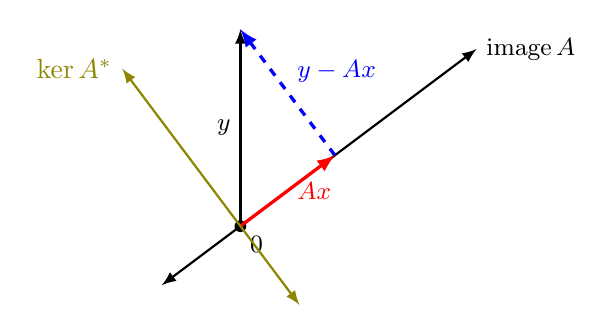
\begin{tikzpicture}
      \draw[thick, latex-latex] (-1,-0.75) -- (3, 2.25);
      \draw[thick, -latex] (0,0) -- (0,2.5) ;
      \node[left] at (0,1.25) {{\small$y$}};
      \node[right] at (3,2.25) {{\small ${\image A}$}};
      \node at (0,0)[circle,fill,inner sep=1.5pt]{};
      \node[below right] at (0,0) {{\small$0$}};
      \draw[-latex, blue, very thick, dashed] (1.2,0.9) -- (0,2.5);
      \node[above right, blue] at (0.6,1.7) {\small $y-Ax$};
      \node[right] at (0.6,0.45) {{\color{red}\small$Ax$}};
      \draw[-latex,red,very thick] (0,0) -- (1.2,0.9);
      \draw[olive,latex-latex,thick] (-1.5,2) node[left] {$\ker A^*$} -- (0.75, -1);
    \end{tikzpicture}
  \end{center}
  \begin{itemize}
  \item If $Ax$ is closest to $y$, then
    \begin{itemize}
    \item $y-Ax$ is orthogonal to $\image A$
    \end{itemize}
  \item Recall that $(\image A)^\perp = \ker A^*$
  \item Therefore, $A$ is closest to $y$ if
    \[
      A^*(y-Ax)) = 0
    \]
    or, equivalently,
    \[
      A^*Ax = A^*y
    \]
  \end{itemize}
\end{frame}

\begin{frame}
  {Example}

  \begin{itemize}
  \item Consider the system of equations
    \begin{align*}
      x + y + z &= 3\\
      x+ y &= 3\\
      z &= 3
    \end{align*}
  \item Equivalently,
    \begin{align*}
      \begin{bmatrix} 1 & 1 & 1 \\ 1 & 1 & 0 \\ 0 & 0 & 1\end{bmatrix}\begin{bmatrix} x \\ y \\ z \end{bmatrix} &= \begin{bmatrix} 3 \\ 3 \\ 3 \end{bmatrix}
    \end{align*}
  \item There is no solution
  \end{itemize}

\end{frame}

\begin{frame}
  {Quasi-Solution}

  \begin{itemize}
  \item Let
    \[
      A = \begin{bmatrix} 1 & 1 & 1 \\ 1 & 1 & 0 \\ 0 & 0 & 1\end{bmatrix}
    \]
  \item $(x,y,z)$ is a quasi-solution if
    \begin{align*}
      A^*A\begin{bmatrix} x \\ y \\ z \end{bmatrix} &= A^*\begin{bmatrix} 3 \\ 3 \\ 3 \end{bmatrix}\\
      \implies \begin{bmatrix} 1 & 1 & 0 \\ 1 & 1 & 0 \\ 1 & 0 & 1\end{bmatrix}
      \begin{bmatrix} 1 & 1 & 1 \\ 1 & 1 & 0 \\ 0 & 0 & 1\end{bmatrix}\begin{bmatrix} x \\ y \\ z \end{bmatrix}
      &= \begin{bmatrix} 1 & 1 & 0 \\ 1 & 1 & 0 \\ 1 & 0 & 1\end{bmatrix}
        \begin{bmatrix} 3 \\ 3 \\ 3 \end{bmatrix}\\
      \implies
      \begin{bmatrix} 2 & 2 & 1 \\ 2 & 2 & 1 \\ 1 & 1 & 2 \end{bmatrix}\begin{bmatrix} x \\ y \\ z \end{bmatrix}
      &= \begin{bmatrix} 6 \\ 6 \\ 6 \end{bmatrix}
    \end{align*}
  \end{itemize}
\end{frame}

\begin{frame}
  {Quasi-Solution Via Row Reduction}

  \begin{itemize}
  \item $(x,y,z)$ is a quasi-solution if
    \begin{align*}
      \begin{bmatrix} 2 & 2 & 1 \\ 2 & 2 & 1 \\ 1 & 1 & 2 \end{bmatrix}\begin{bmatrix} x \\ y \\ z \end{bmatrix}
      &= \begin{bmatrix} 6 \\ 6 \\ 6 \end{bmatrix}\\
      \implies
      \begin{bmatrix} 1 & 1 & 2 \\ 0 & 0 & 3 \\ 0 & 0 & 0\end{bmatrix} \begin{bmatrix} x \\ y \\ z \end{bmatrix}
      &= \begin{bmatrix} 6 \\ 6 \\ 0 \end{bmatrix}\\
      \implies
      \begin{bmatrix} 1 & 1 & 0 \\ 0 & 0 & 1 \\ 0 & 0 & 0\end{bmatrix} \begin{bmatrix} x \\ y \\ z \end{bmatrix}
      &= \begin{bmatrix} 2 \\ 2 \\ 0 \end{bmatrix}\\
      \implies x + y &= 2\\
      z &= 2
    \end{align*}
  \end{itemize}
\end{frame}


\begin{frame}
  {Quasi-Solution Error}

  \begin{itemize}
  \item 
    \begin{align*}
      \begin{bmatrix} x \\ 2-x \\ 2 \end{bmatrix}\text{ is a quasi-solution to }
      \begin{bmatrix} 1 & 1 & 1 \\ 1 & 1 & 0 \\ 0 & 0 & 1\end{bmatrix}\begin{bmatrix} x \\ y \\ z \end{bmatrix} &= \begin{bmatrix} 3 \\ 3 \\ 3 \end{bmatrix}
    \end{align*}
  \item The error of the quasi-solution
    \begin{align*}
      \epsilon &= \begin{bmatrix} 1 & 1 & 1 \\ 1 & 1 & 0 \\ 0 & 0 & 1\end{bmatrix}\begin{bmatrix} x \\ 2-x \\ 2 \end{bmatrix}
                 -\begin{bmatrix} 3 \\ 3 \\ 3 \end{bmatrix}
                 = \begin{bmatrix} 4 \\ 2 \\ 2 \end{bmatrix} - \begin{bmatrix} 3 \\ 3 \\ 3 \end{bmatrix}
                 = \begin{bmatrix} 1 \\ -1 \\ -1 \end{bmatrix} 
    \end{align*}
  \end{itemize}
\end{frame}

\begin{frame}
  {Error Comparison}

  \begin{itemize}
  \item The error for any other $(x,y,z)$ is
    \begin{align*}
      \epsilon &= \begin{bmatrix} 1 & 1 & 1 \\ 1 & 1 & 0 \\ 0 & 0 & 1\end{bmatrix}\begin{bmatrix} x \\ y \\ z \end{bmatrix}
                 -\begin{bmatrix} 3 \\ 3 \\ 3 \end{bmatrix}\\
               &= \begin{bmatrix} x + y + z -3 \\ x + y - 3 \\ z - 3 \end{bmatrix}\\
               &= \begin{bmatrix} 1 \\ -1 \\ -1 \end{bmatrix}
                 + \begin{bmatrix} x+y+z-4 \\ x+y-2 \\ z -2 \end{bmatrix}
    \end{align*}
  \item The error magnitude squared is
    \[
      \epsilon^2 = \left\|\begin{bmatrix} 1 \\ -1 \\ -1 \end{bmatrix}\right\|^2
      + \left\|\begin{bmatrix} x+y+z-4 \\ x+y-2 \\ z -2 \end{bmatrix}\right\|^2
      \ge \left\|\begin{bmatrix} 1 \\ -1 \\ -1 \end{bmatrix}\right\|^2
    \]
  \end{itemize}
\end{frame}

\begin{frame}
  {Quasi-Solutions of $L(x) = y$}

  \begin{itemize}
  \item $L(x)$ is closest to $y$ if
    \[
      L^*L(x) = L^*(y)
    \]
  \item For any $y \in Y$, there is always a quasi-solution $x$, because
    \[
      \image (L^*L) = \image L^*
    \]
    \begin{itemize}
    \item Recall that $\ker (L^*L) = \ker L$
    \item Therefore, since $L^*L$ is self-adjoint,
      \[
        \image (L^*L) = (\ker L^*L)^\perp = (\ker L)^\perp = \image L^*
      \]
    \end{itemize}
  \item If $v \in \ker L^*L =\ker L$, then $x+v$ is also a solution
  \item The quasi-solution is unique only if $\ker L = \{0\}$
    \begin{itemize}
    \item Because the domain and range of $L^*L$ have the same dimension
    \item If $\dim X > \dim Y$, this is not possible, because
      \[
        \dim \ker L = \dim X - \dim (\image L) \ge \dim X - \dim Y > 0
      \]
    \end{itemize}
  \end{itemize}
\end{frame}

\begin{frame}
  {Error Comparison}

  \begin{itemize}
  \item A quasi-solution of the equation $L(x) = y$ satisfies
    \[
      L^*L(x) = L^*(y)
    \]
    and therefore $L^*(L(x) - y) = 0$
  \item The error of the quasi-solution $x$ is
    \[
      \epsilon = L(x) - y
    \]
  \item The error of any $x' \in X$ is
    \[
      \epsilon' = L(x')-y = L(x'-x) + L(x)-y = L(x'-x) + \epsilon
    \]
  \item On the other hand,
    \begin{align*}
      \langle L(x'-x), \epsilon\rangle &= \langle x'-x, L^*(\epsilon)\rangle\\
                                       &= \langle x'-x, L^*L(x) - L^*(y)\rangle\\
                                       &= 0
    \end{align*}
  \item Therefore, $\|\epsilon'\|^2 = \|\epsilon\|^2 + \|L(x'-x)\|^2$
  \end{itemize}
\end{frame}

\begin{frame}
  {Quasi-Solution when $L^*L: X \rightarrow X$ is Invertible}

  \begin{itemize}
  \item If $x$ is a quasi-solution, then
    \[
      L^*L(x) = L^*(y)
    \]
  \item If the map $L^*L: X \rightarrow X$ is invertible, then the unique quasi-solution is
    \[
      x = (L^*L)^{-1}L^*(y)
    \]
  \end{itemize}
\end{frame}

\begin{frame}
  {Solution with Minimal Magnitude}

  \begin{itemize}
  \item Suppose $x \in X$ is a solution (not just a quasi-solution) of
    \[
      Ax = y
    \]
  \item If $v \in \ker A$, then $x + v$ is also a solution,
    \[
      A(x+v) = y
    \]
  \item There is a unique solution $x$ with minimal magnitude
  \end{itemize}
\end{frame}

\begin{frame}
  {Minimal Magnitude Solution Via Orthogonal Projection}

  \begin{itemize}
  \item For any $x' \in X$, there is a unique way to decompose $x'$ into a sum
    \[
      x' = x + (x'-x),
    \]
    where $x \in (\ker A)^\perp$ and $x-x' \in \ker A$
  \item If $x'$ is a solution to
    \[
      Ax' = y,
    \]
    then
    \[
      Ax = A(x-x') + Ax' = y
    \]
  \item If $x_1, x_2 \in (\ker A)^\perp$ are both solutions, then
    \begin{align*}
      x_1-x_2 &\in (\ker A)^\perp\text{ and }x_1 - x_2 \in \ker A,
    \end{align*}
    because
    \[
      A(x_1-x_2) = Ax_1 - Ax_2 = y - y = 0
    \]
    Therefore, $x_1 - x_2 = 0$
  \end{itemize}
\end{frame}

\begin{frame}
  {Quasi-Solution with Minimal Magnitude}

  \begin{itemize}
  \item A quasi-solution to
    \[
      Ax = y
    \]
    is a solution of
    \[
      A^*Ax = A^*y
    \]
  \item There is a unique quasi-solution $x \in (\ker A^*A)^\perp = (\ker A)^\perp$
  \end{itemize}
\end{frame}

\begin{frame}
  {Example}

  \begin{itemize}
  \item The quasi-solutions of the equation
    \begin{align*}
      \begin{bmatrix} 1 & 1 & 1 \\ 1 & 1 & 0 \\ 0 & 0 & 1\end{bmatrix}\begin{bmatrix} x \\ y \\ z \end{bmatrix} &= \begin{bmatrix} 3 \\ 3 \\ 3 \end{bmatrix}
    \end{align*}
    are
    \[
      \begin{bmatrix} x \\ 2-x \\ 2 \end{bmatrix},\ x \in \C
    \]
  \item The magnitude squared of each quasi-solution is
    \begin{align*}
      \left\|\begin{bmatrix} x \\ 2-x \\ 2 \end{bmatrix}\right\|^2
      &= x^2 + (2-x)^2 + 4
        = 2((x-1)^2 + 3)
    \end{align*}
  \item The magnitude is minimized when $x = 1$ and therefore the Moore-Penrose quasi-solution is
    $(1, 1, 2)$
  \end{itemize}
\end{frame}

\begin{frame}
  {Moore-Penrose Quasi-Inverse Operator}

  \begin{itemize}
  \item Let $X$ and $Y$ be inner product spaces and $L: X \rightarrow Y$ be a linear map
  \item There is a map $L^+: Y \rightarrow X$ such that for any $y \in Y$, $x = L^+(y)$ is the unique quasi-solution with minimal magnitude of the equation
    \[
      L(x) = y
    \]
  \item The map $L^+$ is called the {\bf Moore-Penrose quasi-inverse} of $L$
  \end{itemize}
\end{frame}

\begin{frame}
  {Moore-Penrose Quasi-Inverse Operator}

  \begin{itemize}
  \item The map
    \[
      \left.L\right|_{(\ker L)^\perp}: (\ker L)^\perp \rightarrow \image L
    \]
    is an isomorphism.
  \item Let
    \begin{align*}
      \pi: Y &\rightarrow \image L
    \end{align*}
    be orthogonal projection
  \item The Moore-Penrose quasi-inverse operator is the map
    \[
      L^+: Y \rightarrow X,
    \]
    given by
    \[
      L^+(y) = \left(\left.L\right|_{(\ker L)^\perp}\right)^{-1}(\pi(y)) \in (\ker L)^\perp \subset X
    \]
  \end{itemize}
\end{frame}

\begin{frame}
  {Quasi-Inverse of Diagonal Matrix}

  \begin{itemize}
  \item Let $\Sigma: \R^m \rightarrow \R^m$ be the diagonal matrix such that for each $1 \le k \le m$,
    \[ \Sigma(\epsilon_k) = \begin{cases} s_k\epsilon_k &\text{ if }1 \le k \le r\\ 0 &\text{ if }r+1 \le k \le m \end{cases} \]
  \item Therefore,
    \[ \Sigma(\epsilon_1v^1+\cdots+\epsilon_mv^m) = \epsilon_1s_1v^1+\cdots+\epsilon_rs_rv^r \]
  \item The quasi-inverse of $\Sigma$ satisfies the following:
    \[ \Sigma^+(\epsilon_1v^1+\cdots+\epsilon_mv^m) = \epsilon_1s_1^{-1}v^1+\cdots+ \epsilon_rs_rv^r \]
  \item In particular,
    \begin{align*}
      \Sigma^+(\Sigma(\epsilon_1v^1+\cdots+\epsilon_mv^m))
      &= \Sigma^+(\epsilon_1s_1v^1+\cdots+\epsilon_rs_rv^r)\\
      &= \epsilon_1v^1+\cdots+\epsilon_rv^r\\
      &= \pi_r(v),
    \end{align*}
    where $\pi_r: \R^m \rightarrow \R^m$ is orthogonal projection onto the subspace spanned by $(\epsilon_1, \dots, \epsilon_r)$
  \end{itemize}
\end{frame}

\begin{frame}
  {Quasi-Inverse Via Singular Value Decomposition}

  \begin{itemize}
  \item Let the singular value decomposition of $L: X \rightarrow Y$ be
    \[
      L = W\Sigma V^*,
    \]
  \item For each $1 \le k \le m$, let $e_k = V(\epsilon_k)$
  \item For each $1 \le j \le n$, let $f_j = W(\epsilon_j)$
  \item Then for any $x = e_1x^1+\cdots+e_mx^m \in X$,
    \[ L(x) = L(e_1x^1+\cdots+e_mx^m) = f_1s_1x^1+\cdots+f_rs_rx^r \]
  \item Therefore, for any $y = f_1y^1+\cdots+f_ny^n \in Y$,
    \[ L^+(y) = L^+(f_1y^1+\cdots+f_ny^n) = e_1s_1^{-1}y^1+\cdots+e_rs_r^{-1}y^r \]
  \item In other words,
    \[ L^+ = W\Sigma^+V^* \]
  \end{itemize}
\end{frame}

\begin{frame}
  {Image of Unit Ball}

  \begin{itemize}
  \item The closed unit ball centered at the origin in $\R^n$ is
    \[ B = \{ x \in \R^n:\ x\cdot x \le 1 \} \]
  \item Consider the image of $B$ under a linear map $A: \R^n \rightarrow \R^n$
  \item If $A$ is diagonal, then if $y = Ax \in AB$,
    \begin{align*}
      Ay &= A\begin{bmatrix}x^1 \\ x^2 \\ \vdots \\ x^n \end{bmatrix}
           = \begin{bmatrix} d^1 & 0 & \cdots & 0 \\ 0 & d^2 & \cdots & 0 \\ \vdots & \vdots & \ddots & \vdots \\ 0 & 0 & \cdots & d^n \end{bmatrix}\begin{bmatrix}x^1 \\ x^2 \\ \vdots \\ x^n \end{bmatrix}
           = \begin{bmatrix} d^1x^1 \\ d^2x^2 \\ \vdots \\ d^nx^n \end{bmatrix}
    \end{align*}
  \item Therefore, $y \in AB$ if and only if
    \[
      1 \ge (x^1)^2 + \cdots + (x^n)^2 = \left(\frac{y^1}{d^1}\right)^2 + \cdots + \left(\frac{y^n}{d^n}\right)^2
    \]
    
  \end{itemize}
\end{frame}

\begin{frame}
  {Ellipse}

  \begin{center}
    \scalebox{0.5}{
      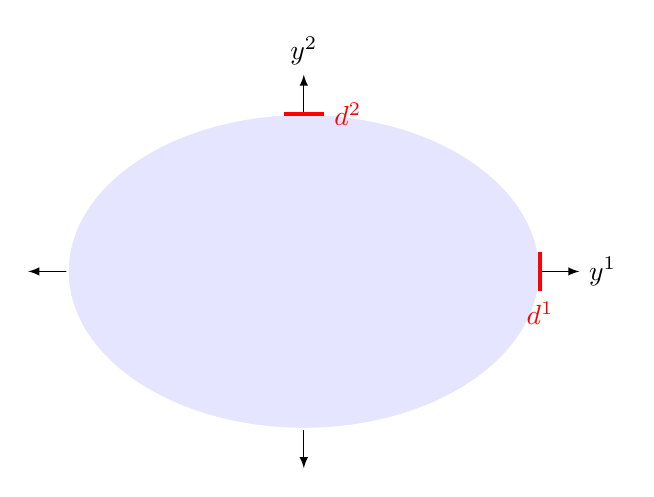
\begin{tikzpicture}
        \draw[latex-latex] (-3.5,0)--(3.5,0) node [right] {$y^1$};
        \draw[latex-latex] (0,-2.5)--(0,2.5) node [above] {$y^2$};
        \draw[white, thick, fill=blue!10] (0,0) circle [x radius = 3, y radius = 2];
        \draw[red,very thick] (3,0.25) -- (3,-0.25) node [below] {$d^1$};
        \draw[red,very thick] (-0.25,2) -- (0.25,2) node [right] {$d^2$};
      \end{tikzpicture}
    }
  \end{center}

  \begin{itemize}
  \item If
    \[
      y = \begin{bmatrix} y^1 \\ y^2 \end{bmatrix}
      = \begin{bmatrix} d^1 & 0 \\ 0 & d^2 \end{bmatrix}
      \begin{bmatrix} x^1 \\ x^2 \end{bmatrix} = Ax
    \]
    then
    \begin{align*}
      x \in B \iff \frac{(y^1)^2}{(d^1)^2} + \frac{(y^2)^2}{(d^2)^2} \le 1
    \end{align*}
  \end{itemize}
\end{frame}


\begin{frame}
  {$3$-Dimensional Ellipsoid}

  \begin{center}
    \scalebox{0.5}{
      \newcommand{\asa}{2}
      \newcommand{\bsa}{0.5}
      \newcommand{\csa}{0.75}
      % view angle
      \tdplotsetmaincoords{70}{135}
      % 
      \begin{tikzpicture}[scale=2,tdplot_main_coords,line join=bevel,fill opacity=.8]
        \pgfsetlinewidth{.1pt}
        \tdplotsphericalsurfaceplot[parametricfill]{72}{36}%
        {1/sqrt((sin(\tdplottheta))^2*(cos(\tdplotphi))^2/\asa+
          (sin(\tdplottheta))^2*(sin(\tdplotphi))^2/\bsa + (cos(\tdplottheta))^2/\csa)} % function defining radius
        {black} % line color
        {2*\tdplottheta} % fill
        {\draw[color=black,thick,->] (0,0,0) -- (2,0,0) node[anchor=north east]{$y^1$};}% x-axis
        {\draw[color=black,thick,->] (0,0,0) -- (0,1.5,0) node[anchor=north west]{$y^2$};}% y-axis
        {\draw[color=black,thick,->] (0,0,0) -- (0,0,1) node[anchor=south]{$y^3$};}% z-axis
      \end{tikzpicture}
    }
  \end{center}

  \begin{align*}
    \frac{(y^1)^2}{(d^1)^2} + \frac{(y^2)^2}{(d^2)^2} + \frac{(y^3)^2}{(d^3)^2} \le 1
  \end{align*}
\end{frame}

\begin{frame}
  {$n$-Dimensional Ellipsoid in $\mathbb{R}^n$}

  \begin{itemize}
  \item Given $d^1, \dots, d^n \ne 0$,
    \[
      E = \left\{ (y^1, \dots, y^n) \in \R^n:\
        \frac{(y^1)^2}{(d^1)^2} + \cdots + \frac{(y^n)^2}{(d^n)^2} \le 1 \right\}
    \]
    is called an $n$-dimensional {\bf ellipsoid}
  \item If $A$ is a diagonal matrix with nonzero diagonal entries $d^1, \dots, d^n$, then
    \begin{align*}
      AB &= E\\
         &= \{ y \in \R^n:\ (A^{-1}y,A^{-1}y) \le 1 \}
    \end{align*}
  \end{itemize}
\end{frame}

\begin{frame}
  {Ellipsoids in Inner Product Space}

  \begin{itemize}
  \item A subset $E$ of an $n$-dimensional real inner product space is an $n$-dimensional {\bf ellipsoid} if there is a unitary basis $(u_1, \dots, u_n)$ and nonzero scalars $d_1, \dots, d_n$ such that
    \[ E = \left\{ y^1u_1+\cdots+y^nu_n:\ \frac{(y^1)^2}{(d^1)^2} + \cdots + \frac{(y^n)^2}{(d^n)^2} \le 1 \right\} \]
  \item A subset $E$ of an $n$-dimensional realinner product space is an $k$-dimensional {\bf ellipsoid} if there is a unitary set $(u_1, \dots, u_k)$ and nonzero scalars $d_1, \dots, d_k$ such that
    \[ E = \left\{ y^1u_1+\cdots+y^nu_k:\ \frac{(y^1)^2}{(d^1)^2} + \cdots + \frac{(y^k)^2}{(d^k)^2} \le 1 \right\} \]
  \end{itemize}
  
\end{frame}

\begin{frame}
  {Unitary Transformation of Ball is Ball}

  \begin{itemize}
  \item If $X$ and $Y$ are inner product spaces with the same dimension, a map $U: X \rightarrow Y$ is a unitary transformation, if, for any $v \in X$,
    \[
      (U(x),U(x))_Y = (x,x)_X
    \]
  \item Therefore, if
    \[ B_X = \{ x\in X:\ (x,x) = 1 \}, \]
    then
    \[ U(B_X) \subset B_Y \]
  \item On the other hand, if $y \in B_Y$, then $U^*(y)) \in B_X$ and $U(U^*(x)) = x$, which implies
    \[ B_Y \subset U(B_X) \]
  \item It follows that $U(B_X) = B_Y$
  \end{itemize}
\end{frame}

\begin{frame}
  {Singular Value Decomposition}

  \begin{itemize}
  \item Let $X$ and $Y$ be real inner product spaces such that $\dim(X) = m$ and $\dim(Y) = n$
  \item $L: X \rightarrow Y$ be a linear transformation
  \item The singular value decomposition of $L$ can be described as follows:
    \begin{itemize}
    \item There exists a unitary basis $(e_1, \dots, e_m)$ of $X$ and a unitary basis $(f_1, \dots, f_n)$  of $Y$ such that if $r = \rank(L)$, then
      \[
        L(e_k) =
        \begin{cases}
          s_kf_k &\text{ if }1 \le k \le r\\
          0 &\text{ if }r+1 \le k \le m
        \end{cases},
      \]
      where $s_1, \dots, s_n$ are the singular values of $L$
    \item In particular, $(e_1, \dots, e_r)$ is a unitary basis of $(\ker(L))^\perp$ and $(f_1, \dots, f_r)$ is a unitary basis of $\image(L)$
    \end{itemize}
  \end{itemize}
\end{frame}

\begin{frame}
  {Linear Transformation of Ball is an Ellipsoid (Part 1)}

  \begin{itemize}
  \item The unit ball is
    \[ B = \{ x^1e_1+\cdots+x^ne_n: \ (x^1)^2 + \cdots + (x^n)^2 \le 1\} \]
  \item If $x \in B$, then
    \begin{align*}
      L(x) &= x^1L(e_1) + \cdots + x^nL(e_n)\\
           &= s_1x^1 f_1 + \cdots + s_rx^rf_r\\
           &= y^1f_1 + \cdots + y^rf_r,
    \end{align*}
    where
    \[ \frac{(y^1)^2}{(s_1)^2} + \cdots + \frac{(y^r)^2}{(s_r)^2} = (x^1)^2 + \cdots + (x^r)^2 \le 1 \]
  \end{itemize}
\end{frame}

\begin{frame}
  {Linear Transformation of Ball is an Ellipsoid (Part 2)}

  \begin{itemize}
  \item The set
    \begin{align*}
      E &= \left\{ y^1f_1 + \cdots + y^rf_r:\ \frac{(y^1)^2}{(s_1)^2} + \cdots + \frac{(y^n)^2}{(s_r)^2}\right.\\
        &\quad= \left.(x^1)^2 + \cdots + (x^r)^2 \le 1 \right\} \subset \image(L)
    \end{align*}
    is an $r$-dimensional ellipsoid in $Y$ such that
    \[ L(B_X) \subset E \]
  \end{itemize}
\end{frame}

\begin{frame}
  {Linear Transformation of Ball is an Ellipsoid (Part 3)}

  \begin{itemize}
  \item 
    Conversely, if $y = y^1f_1 + \cdots + y^rf_r \in E$, then
    \[
      L(x) = y,
    \]
    where
    \[
      x = \left(\frac{y^1}{s_1}\right)e_1 + \cdots + \left(\frac{y^r}{s_r}\right)e_n \in B
    \]
  \item It follows that $E \subset L(B)$
  \item Therefore, $E = L(B)$
  \end{itemize}
\end{frame}

\begin{frame}
  {Operator Norm of Linear Map}

  \begin{itemize}
  \item Let $X$ and $Y$ be inner product spaces and $L: X \rightarrow Y$ be a linear map
  \item The {\bf operator norm} of $L$ is defined to be
    \[
      \|L\| = \sup \{ |L(x)|\ :\ x \in B_X \}
    \]
  \item Let $s_1 \le s_2 \le \cdots \le s_r$ be the singular values of $L$
  \item For any $x = x^1e_1 + \cdots + x^me_m \in B$,
    \begin{align*}
      (L(x),L(x)) &= (x^1s_1f_1 + \cdots + x^rs_r f_r,x^1s_1f_1 + \cdots + x^rs_r f_r) \\
                  &= (s_1)^2(x^1)^2 + \cdots + (s_r)^2(x^r)^2\\
                  &\le (s_r)^2((x^1)^2 + \cdots + (x^r)^2)\\
                  &\le (s_r)^2
    \end{align*}
  \item Moreover,
    \[ (L(e_r),L(e_r)) = (s_rf_r,s_rf_r) = (s_r)^2 \]
  \item Therefore, $\|L\|$ is equal to the largest singular value of $L$
  \end{itemize}
\end{frame}

\begin{frame}
  {Change of Basis Formula}
  \begin{itemize}
  \item Let $L: X \rightarrow X$ be a linear endomorphism (codomain is domain)
  \item Given a basis $E (e_1, \dots, e_m)$ of $X$, there is a matrix $M$ such that
    \[
      L(e_k) = M_k^je_j, i.e., L(E) = EM
    \]
  \item If $F = (f_1,\dots, f_m)$ is another basis such that
    \[
      f_k = A_k^je_j,\ i.e., F = EA,
    \]
    then
    \[
      L(F) = L(EA) = L(E)A = EMA = FA^{-1}MA
    \]
  \end{itemize}
\end{frame}

\begin{frame}
  {Trace of a Linear Endomorphism}

  \begin{itemize}
  \item If $L(E) = EM$, then the trace of $L$ is defined to be
    \[
      \trace(L) = M^1_1 + \cdots + M^m_m
    \]
  \item If $L(F) = EN$, then $N = A^{-1}MA$, i.e.,
    \[
      N^l_k = (A^{-1})^l_iM^i_jA^j_k
    \]
  \item Therefore,
    \begin{align*}
      N_1^1 + \cdots + N^m_m &= N^k_k\\
                             &= (A^{-1})^k_iM^i_jA^j_k\\
                             &= A^j_k(A^{-1})^k_iM^i_j\\
                             &= \delta^j_iM^i_j\\
                             &= M^j_j\\
                             &= M^1_1 + \cdots + M^m_m
    \end{align*}
  \item The definition of $\trace(L)$ does not depend on the basis used
  \end{itemize}
\end{frame}

\begin{frame}
  {Frobenius Norm of a Linear Transformation}

  \begin{itemize}
  \item Let $X$ and $Y$ be real inner product spaces
  \item Let $L: X \rightarrow Y$ be a linear map
  \item Recall that the adjoint of $L$ is the map $L^*: Y \rightarrow X$ such that for any $x \in X$ and $y \in Y$,
    \[
      (L(x),y) = (x,L^*(y))
    \]
  \item The {\bf Frobenius norm} or {\bf Hilbert-Schmidt norm} of $L$ is defined to be $\|L\|_2$, where
    \[ \|L\|_2^2 = \trace(L^*L) \]
  \end{itemize}
\end{frame}

\begin{frame}
  {Frobenius Norm With Respect to Basis}

  \begin{itemize}
  \item Let $(e_1, \dots, e_m)$ be a unitary basis of $X$ and $(f_1, \dots, f_n)$ be a unitary basis of $Y$ such that
    \[
      L(e_k) =
      \begin{cases}
        s_kf_k &\text{ if }1 \le k \le r\\
        0 &\text{ if }r+1 \le k \le m,
      \end{cases}
    \]
  \item The adjoint of $L$ is given by
    \[
      L^*(f_k) =
      \begin{cases}
        s_ke_k &\text{ if }1 \le k \le r\\
        0 &\text{ if }r+1 \le k \le n
      \end{cases}
    \]
  \item Therefore,
    \begin{align*}
      L^*L(e_k) = 
      \begin{cases}
        s_k^2e_k &\text{ if }1 \le k \le r\\
        0 &\text{ if }r+1 \le k \le m
      \end{cases}
    \end{align*}
  \item It follows that
    \[
      \|L\|_2^2 = \trace(L^*L) = s_1^2 + \cdots + s_r^2
    \]
  \item Observe that the operator norm is always less than or equal to the Frobenius norm,
    \[ \|L\| = \max(s_1, \dots, s_r) \le \sqrt{s_1^2 + \cdots + s_r^2} = \|L\|_2 \]
    and equality holds if and only if the rank of $L$ is $1$
  \item On the other hand,
    \[ \|L\|_2^2 = s_1^2 + \cdots + s_r^2 \le r(\max(s_1, \dots, s_r))^2 = r\|L\|^2 \],
    i.e.,
    \[ \|L\|_2 \le \sqrt{r}\|L\|, \]
    where equality holds if and only if $s_1 = \cdots = s_r$
  \end{itemize}
\end{frame}

\begin{frame}
  {Solving a Linear System with Errors}

  \begin{itemize}
  \item Let $L: X \rightarrow Y$ be a linear map between inner product spaces
  \item Suppose that, given $y \in Y$, we want to solve
    \[ L(x) = y, \]
    for $x$ but the exact value of $y$ is not known
  \item If the measured value of $y$ is $y + \Delta y$ and
    \[ x + \Delta x = L^{-1}(y+\Delta y), \]
    then
    \[
      \Delta x = L^{-1}(\Delta y)
    \]
  \item The relative error of $x$ can ye estimated in terms of the relative error of $y$:
    \[ \frac{|\Delta x|}{|x|} = \frac{|L^{-1}(\Delta y)|}{|y|}\frac{|y|}{|x|}
      = \frac{|L^{-1}(\Delta y)|}{|y|}\frac{|L(x)|}{|x|}
      \le \|L^{-1}\|\|L\|\frac{|\Delta y|}{|y|} \]
  \end{itemize}
\end{frame}

\begin{frame}
  {Condition Number of Linear Map}

  \begin{itemize}
  \item $\|L^{-1}\|\|L\|$ is the {\bf condition number} of the linear map
  \item It shows how sensitive the error in $x$ is to the error in $y$
  \item A linear map is {\bf ill-conditioned} if the condition number is large
  \item The condition number can be changed by changing the inner product
  \end{itemize}
\end{frame}

\begin{frame}
  {Natural Isomorphism of Inner Product Space and Dual}

  \begin{itemize}
  \item Let $V$ be an inner product space
  \item There is a natural map
    \begin{align*}
      \delta: V &\rightarrow V^*\\
      w &\mapsto \ell_w,
    \end{align*}
    where for any $v \in V$,
    \[
      \langle\ell_w,v\rangle = (v,w)
    \]
  \item $w$ is in the kernel of this map if $\ell_w = 0$, i.e., for any $v \in V$,
    \[
      0 = \langle\ell_w,v\rangle = (v,w)
    \]
    This holds if and only if $w = 0$
  \end{itemize}
\end{frame}

\begin{frame}
  {Bilinear Form on Real Vector Space}

  \begin{itemize}
  \item A {\bf bilinear form} on a real vector space $V$ is a bilinear function
    \[ B: V\times V \rightarrow \R \]
  \item I.e., for any $a^1, a^2 \in \R$ and $v_1, v_2, v \in V$,
    \begin{align*}
      B(a^1v_1+a^2v_2,v) &= a^1B(v_1,v)+a^2B(v_2,v)\\
      B(v,a^1v_1+a^2v_2) &= a^1B(v,v_1)+a^2B(v,v_2)
    \end{align*}
  \item An inner product is an example of a bilinear form
  \end{itemize}
\end{frame}

\begin{frame}
  {Bilinear Form on Inner Product Space}

  \begin{itemize}
  \item Given a linear map $L: V \rightarrow V$, the function
    \begin{align*}
      B: V\times V &\rightarrow \R\\
      (v_1,v_2) &\mapsto (L(v_1),v_2)
    \end{align*}
    is a bilinear form
  \item Conversely, if $B: V\times V\rightarrow \R$ is a bilinear form, then there is a map
    \begin{align*}
      \delta_B: V &\rightarrow V^*\\
      w &\mapsto \ell_w,
    \end{align*}
    where for any $v \in V$,
    \[ \langle\ell_w,v\rangle = B(v,w) \]
  \item If $V$ has an inner product and
    \[ L = (\delta^{-1}\circ\delta_B)^*: V \rightarrow V, \]
    then
    \[
      B(v,w) = \langle\delta_B(w),v\rangle = (v,\delta^{-1}(\delta_B(w))) = (L(v),w))
    \]
  \end{itemize}
\end{frame}

\begin{frame}
  {Bilinear Form as Matrix}

  \begin{itemize}
  \item If $(e_1, \dots, e_n)$ is a basis of $V$ and
    \[ v = e_jv^j\text{ and }w = e_kw^k, \]
    then
    \begin{align*}
      B(v,w) &= B(e_jv^j, e_kw^k)\\
             &= v^jw^kB(e_j,e_k)\\
             &= v^jw^kM_{jk}
    \end{align*}
  \item Therefore, given a basis $(e_1, \dots, e_n)$ of $V$, $B$ is uniquely determined by the $n$-by-$n$ matrix $M$, where
    \[ M_{jk} = B(e_j,e_k) \]
  \item Conversely, given any $n$-by-$n$ matrix $M$, we can define a bilinear form $B$, where
    \[
      B(e_jv^j,e_kw^k) = M_{jk}v^jw^k
    \]
  \item Two bilinear forms are equal if and only if their matrices (with respect to a basis) are equal
  \end{itemize}
\end{frame}

\begin{frame}
  {Symmetric Bilinear Forms}

  \begin{itemize}
  \item A bilinear form $B$ on a real vector space $V$ is {\bf symmetric} if for any $v_1, v_2 \in V$,
    \[ B(v_2,v_1) = B(v_1,v_2) \]
  \item Given a basis $(e_1, \dots, e_n)$ of $V$, a bilinear form $B$ is symmetric if and only if 
    \[
      B(e_jv^j,e_kw^k) = M_{jk}v^jw^k\text{ and }M_{kj} = M_{jk}
    \]
  \item An inner product on $V$ is an example of a bilinear form
  \end{itemize}
\end{frame}

\begin{frame}
  {Quadratic Form on Real Vector Space}

  \begin{itemize}
  \item A function $Q: V \rightarrow \R$ is a {\bf quadratic form} if there exists a symmetric bilinear form $B: V\times V\rightarrow \R$ such that for each $v \in V$,
    \[
      Q(v) = B(v,v)
    \]
  \item Equivalently, if $(e_1, \dots, e_n)$ is a basis of $V$, then there exist coefficients $b_{ij}=b_{ji}$, $1 \le i,j \le n$, such that for any $v = e_kv^k$,
    \[ Q(v,v) = b_{ij}v^iv^j \]
  \item Examples:
    \begin{itemize}
    \item
      \begin{align*}
        Q(e_1x^1+e_2x^2+e_3x^3) &= (x^1)^2 + (x^2)^2 - (x^3)^2\\
        Q(e_1x^1+e_2x^2+e_3x^3) &= x^1x^2
      \end{align*}
    \end{itemize}
  \item The right side is always a homogeneous polynomial of degree $2$
    \begin{itemize}
    \item Homogeneous means every term has same degree
    \end{itemize}
  \end{itemize}
\end{frame}

\begin{frame}
  {Inner Product on Complex Vector Space}

  \begin{itemize}
  \item Inner product on complex vector space $V$ looks different from one on real vector space
  \item For any $v, v_1, v_2 \in V$ and $c \in \C$,
    \begin{align*}
      (v_1+v_2,v) &= (v_1,v) + (v_2,v)\\
      (v, v_1+v_2) &= (v,v_1) + (v,v_2)\\
      (cv_1,v_2) &= c(v_1,v_2)\\
      (v_1,cv_2) &= \bar{c}(v_1,v_2)
    \end{align*}
  \end{itemize}
\end{frame}

\begin{frame}
  {Sesquilinear Form on Complex Vector Space}

  \begin{itemize}
  \item A sesquilinear form is a function
    \[ B: V\times V\rightarrow \C \]
    with the following properties, similar to above:
    \begin{align*}
      B(v_1+v_2,v) &= B(v_1,v) + B(v_2,v)\\
      B(v, v_1+v_2) &= B(v,v_1) + B(v,v_2)\\
      B(cv_1,v_2) &= cB(v_1,v_2)\\
      B(v_1,cv_2) &= \bar{c}B(v_1,v_2)
    \end{align*}
  \end{itemize}
\end{frame}

\begin{frame}
  {Space of Linear Maps and Space of Sesquilinear Forms}

  \begin{itemize}
  \item Let $V$ be an inner product space
  \item Let $\mathcal{L}(V)$ be the space of all linear maps $L: V \rightarrow V$
  \item If $L_1, L_2 \in \mathcal{L}(V)$ and $c^1, c^2 \in \F$, then
    \[ c^1L_1+c^2L_2 \in \mathcal{L}(V) \]
  \item Let $\mathcal{B}(V)$ be the space of all sesquilinear forms $B: V \times V\rightarrow \F$
  \item If $B_1, B_2 \in \mathcal{L}(V)$ and $c^1, c^2 \in \F$, then
    \[ c^1B_1+c^2B_2 \in \mathcal{B}(V) \]
  \end{itemize}
\end{frame}

\begin{frame}
  {Isomorphism between Spaces of Linear Maps and of Sesquilinear Forms}

  \begin{itemize}
  \item There is a linear map $\mathcal{L}(V) \rightarrow \mathcal{B}(V)$, where each $L \in \mathcal{L}(V)$ maps to $B \in \mathcal{V}$ such that for any $v,w \in V$,
    \[ B(v,w) = (L(v),w) \]
  \item If $L$ lies in the kernel of this map, then for any $v,w \in V$, $B = 0$ and therefore
    \[ 0 = B(v,w) = (L(v),w) \]
  \item This implies that $L(v) = 0$ for any $v \in V$, which implies $L = 0$
  \item Given $B \in \mathcal{B}(V)$ and $w \in V$, 
  \end{itemize}
\end{frame}


\begin{frame}
  {Sesquilinear Form as Matrix}

  \begin{itemize}
  \item If $(e_1, \dots, e_n)$ is a basis of $V$ and $v = e_jv^j,\ w = e_kw^k,$
    then
    \begin{align*}
      B(v,w) &= B(e_jv^j, e_kw^k)\\
             &= v^j\bar{w}^kB(e_j,e_k)\\
             &= v^j\bar{w}^kM_{jk}
    \end{align*}
  \item Therefore, given a basis $(e_1, \dots, e_n)$ of $V$, $B$ is uniquely determined by the $n$-by-$n$ matrix $M$, where
    \[ M_{jk} = B(e_j,e_k) \]
  \item Conversely, given any $n$-by-$n$ matrix $M$, we can define a bilinear form $B$, where
    \[
      B(e_jv^j,e_kw^k) = M_{jk}v^jw^k
    \]
  \item Two bilinear forms are equal if and only if their matrices (with respect to a basis) are equal
  \item Sometimes, we write
    \[  M_{j\bar{k}} = B(e_j,e_k) \]
    to keep track of the fact that
    \[
      B(v,w) = v^jM_{j\bar{k}}\bar{w}^k
    \]
  \end{itemize}
\end{frame}

\begin{frame}
  {Different Notation Conventions}

  \begin{itemize}
  \item We are using the following convention:
    \begin{align*}
      B(cv,w) &= cB(v,w)\\
      B(v,cw) &= \bar{c}B(v,w)
    \end{align*}
  \item Some use the following convention:
    \begin{align*}
      B(cv,w) &= \bar{c}B(v,w)\\
      B(v,cw) &= cB(v,w)
    \end{align*}
  \item When reading a paper or book, look carefully to see which convention is used
  \end{itemize}
\end{frame}

\begin{frame}
  {Hermitian Forms}

  \begin{itemize}
  \item A sequilinear form $B$ on a complex vector space $V$ is {\bf hermitian} if for any $v_1, v_2 \in V$,
    \[ B(v_2,v_1) = \overline{B(v_1,v_2)} \]
  \item Given a basis $(e_1, \dots, e_n)$ of $V$, $B$ is hermitian if and only if its matrix $M_{jk} = B(e_j,e_k)$ satisfies
    \[
      M_{kj} = \bar{M}_{jk}
    \]
  \item An inner product on $V$ is an example of a hermitian form
  \end{itemize}
\end{frame}

\begin{frame}
  {Quadratic Form on Complex Vector Space}

  \begin{itemize}
  \item A function $Q: V \rightarrow \R$ is a {\bf quadratic form} if there exists a hermitian form $B: V\times V\rightarrow \C$ such that for each $v \in V$,
    \[
      Q(v) = B(v,v)
    \]
  \item Equivalently, if $(e_1, \dots, e_n)$ is a basis of $V$, then
    there is a hermitian matrix $M$ such that for any $v = e_kv^k$,
    \[ Q(v,v) = M_{ij}v^i\overline{v}^j \]
  \end{itemize}
\end{frame}

\begin{frame}
  {Example}
  
  \begin{itemize}
  \item If $Q(e_1v^1+e_2v^2+e_3v^3) = |v^1|^2 + |v^2|^2 - |v^3|^2$, then $Q(v) = B(v,v)$, where
    \begin{align*}
      B(e_1,e_1) &= 1\\
      B(e_2,e_2) &= 1\\
      B(e_3,e_3) &= -1\\
      B(e_2,e_3) &= B(e_3,e_1) = B(e_1,e_2) = 0
    \end{align*}
  \end{itemize}
\end{frame}

\begin{frame}
  {Example}
  
  \begin{itemize}
  \item If $Q(e_1v^1+e_2v^2+e_3v^3) = v^1\bar{v}^2$, then $Q(v) = B(v,v)$, where
    \begin{align*}
      B(e_1,e_1) &= 0\\
      B(e_2,e_2) &= 0\\
      B(e_1,e_2) &= B(e_2,e_1) = \frac{1}{2}\\
      B(e_2,e_3) &= B(e_3,e_1) = 0
    \end{align*}
  \end{itemize}
\end{frame}

\begin{frame}
  {Example}
  
  \begin{itemize}
  \item If $Q(e_1v^1+e_2v^2+e_3v^3) = iv^1\bar{v}^2$, then $Q(v) = B(v,v)$, where
    \begin{align*}
      B(e_1,e_1) &= 0\\
      B(e_2,e_2) &= 0\\
      B(e_1,e_2) &= \frac{i}{2}\\
      B(e_2,e_1) &= -\frac{i}{2}\\
      B(e_2,e_3) &= B(e_3,e_1) = 0
    \end{align*}
  \end{itemize}
\end{frame}

\begin{frame}
  {Hermitian Form as $(1,1)$-Polynomial}

  \begin{itemize}
    
  \item Observe that
    \begin{align*}
      Q(e_kx^k) &= B(e_jx^j,e_kx^k)\\
                &= x^j\bar{x}^kB(e_j,e_k)\\
                &= M_{jk}x^j\bar{x}^k,
    \end{align*}
    \begin{itemize}
    \item which is called a polynomial of degree $(1,1)$
    \end{itemize}
  \end{itemize}
\end{frame}

\begin{frame}
  {Change of Basis Formula for Quadratic Form}

  \begin{itemize}
  \item On a complex vector space $V$, let $Q$ be a quadratic form.
    $E = (e_1, \dots, e_n)$ be a basis of $V$, and $M$ be the hermitian matrix such that
    \[
      Q(e_kv^k) = v^j\bar{v}^kM_{jk}
    \]
  \item If $F = (f_1, \dots, f_n)$ is another basis such that
    \[
      f_k = e_jA_k^j,
    \]
    then
    \begin{align*}
      Q(f_pw^p) &= Q(e_jA^j_pw^p)\\ &= B(e_jA^j_pw^p,e_kA^k_qw^q)\\
                &= w^pA^j_pB(e_j,e_k)\bar{A}^k_q\bar{w}^q\\
                &= w^p\bar{w}^q N_{pq},
    \end{align*}
    where
    \[ N_{pq} = A^j_pM_{jk}\bar{A}^k_q\text{, i.e., } N = AMA^*\]
  \end{itemize}
\end{frame}

\begin{frame}
  {Diagonalization of a Quadratic Form}

  \begin{itemize}
  \item Recall that since $M$ is a hermitian matrix, its eigenvalues are real and there exists a unitary matrix $U$ such that
    \[ M = UDU^*, \]
    where $D$ is a diagonal matrix with the eigenvalues of $M$ along its diagonal
  \item In particular, if
    \[ e_p = f_kU^k_p, \]
    then
    \begin{align*}
      Q(f_j,f_k) &= Q(e_pU^p_j,e_qU^q_k)\\
                 &= U^p_jQ(e_p,e_q)U^q_k\\
                 &= U^p_jM_{pq}U^q_k\\
                 &= (U^*MU)_{jk}\\
                 &= D_{jk}
    \end{align*}
  \item Observe that no inner product on $V$ is used here
  \end{itemize}
\end{frame}

\begin{frame}
  {Example (Part 1)}

  \begin{itemize}
  \item Let
    \begin{align*}
      Q(e_1x +e_2y) &= ax^2 + 2bxy + cy^2,
    \end{align*}
    where $a \ne 0$
  \item Then, completing the square,
    \begin{align*}
      Q(e_1x +e_2y) &= ax^2 + 2bxy + cy^2\\
                    &= a\left(x + \frac{b}{a}y\right)^2 + \left(c-\frac{b^2}{a}\right)y^2
    \end{align*}
  \end{itemize}
\end{frame}

\begin{frame}
  {Example (Part 2)}

  \begin{itemize}
  \item If
    \begin{align*}
      f_1 &= e_1\text{ and }f_2 = -\alpha e_1+ e_2,
    \end{align*}
    then
    \begin{align*}
      Q(f_1u+f_2v) &= Q(e_1u + (-\alpha e_1+e_2)v)\\
                   &= Q((u-\alpha v)e_1+ ve_2)\\
                   &= a(u-\alpha v)^2 + 2b(u-\alpha v)v + cv^2)\\
                   &= au^2 + 2(-\alpha a + b)uv + (a\alpha^2 -2b \alpha + c)v^2
    \end{align*}
  \item Therefore, if we assume $a \ne 0$ and set
    \[
      \alpha =  \frac{b}{a},
    \]
    then
    \[
      Q(f_1u+f_2v) = au^2 + \left(c-\frac{b^2}{a}\right)v^2
    \]
  \end{itemize}
\end{frame}

\begin{frame}
  {Example (Part 3)}

  \begin{itemize}
  \item If
    \[ g_1 = pf_1\text{ and }g_2 = qf_2, \]
    then
    \begin{align*}
      Q(g_1 s + g_2t) &= Q(pf_1 s + qf_2t)\\
                      &= (ap^2)s^2 + q^2\left(c-\frac{b^2}{a}\right)t^2
    \end{align*}
  \item It follows that if $p$ and $q$ are chosen appropriately,  then
    \[
      Q(g_1s+g_2t) =
      \begin{cases}
        s^2 + t^2 &\text{ if }a > 0\text{ and }ac - b^2 > 0\\
        s^2 &\text{ if }a > 0\text{ and }ac-b^2=0\\
        s^2 - t^2 &\text{ if }a > 0\text{ and }ac - b^2 < 0\\
        -s^2 + t^2 &\text{ if }a < 0\text{ and }ac - b^2 < 0\\
        -s^2 &\text{ if }a < 0\text{ and }ac - b^2 = 0\\
        -s^2 - t^2 &\text{ if }a < 0\text{ and }ac - b^2 > 0
      \end{cases}
    \]
  \end{itemize}
\end{frame}

\begin{frame}
  {Signature of Quadratic Form}

  \begin{itemize}
  \item The {\bf signature} of a diagonal matrix is $(a,b,c)$, where $a$ is the number of positive diagonal elements, $b$ is the number of negative diagonal elements, and $c$ is the number of zero diagonal elements
  \item {\bf Sylvester's Law of Inertia:} Any two diagonalizations of a quadratic form has the same signature
  \end{itemize}
\end{frame}

\begin{frame}
  {Sylvester's Law of Inertia}
  
  \begin{itemize}
  \item Let $Q: V \rightarrow \R$ be a quadratic form
  \item Let $(e_1, \dots, e_n)$ and $(f_1, \dots, f_n)$ be bases of $V$ that diagonalize $Q$
  \item I.e., for any $v = e_ka^k = f_kb^k$,
    \begin{align*}
      Q(v) &= Q(e_ka^k)\\
           &= \alpha_1(a^1)^2 + \cdots + \alpha_n(a^n)^2\\
           &= Q(f_kb^k)\\
           &= \beta_1(b^1)^2 + \cdots + \beta_n(b^n)^2
    \end{align*}
  \item We want to show that the number of positive values in $\{a^1, \dots, a^n\}$ equals the number of positive values in $\{b^1,\dots, b^n\}$
  \item The same argument will also imply that the number of negative values in $\{a^1, \dots, a^n\}$ equals the number of negative values in $\{b^1,\dots, b^n\}$
  \end{itemize}
\end{frame}

\begin{frame}
  {Proof (Part 1)}

  \begin{itemize}
  \item Let $r$ be the number of positive values in $\{e_1, \dots, e_n\}$
  \item We can assume that
    \begin{align*}
      \alpha_k &= Q(e_k,e_k)
                 \begin{cases}
                   > 0 &\text{ if }1 \le k \le r\\
                   \le 0 &\text{ if }r+1 \le k \le n
                 \end{cases}
    \end{align*}
  \item Let $R$ be the subspace spanned by $\{e_1,\dots, e_{r}\}$
  \item Similarly, let $s$ be the number of positive values in $\{f_1, \dots, f_n\}$ and assume that
    \begin{align*}
      \beta_k &= Q(f_k,f_k)
                \begin{cases}
                  > 0 &\text{ if }1 \le k \le s\\
                  \le 0 &\text{ if }s+1 \le k \le n
                \end{cases}
    \end{align*}
  \item Let $S$ be the subspace spanned by $\{f_1, \dots, f_s\}$
  \end{itemize}
\end{frame}

\begin{frame}
  {Proof (Part 2)}

  \begin{itemize}
  \item Define the projection map
    \begin{align*}
      P: V &\rightarrow R\\
      v=e_1v^1+\cdots+e_nv^n &\mapsto e_1v^1+\cdots+e_{r}v^{r}
    \end{align*}
  \item Let $P_S: S \rightarrow R$ be the restriction of $P$ to $S$
  \item On one hand, if $v \in S$, then $v = f_1b^1+\cdots+f_sb^s$ and
    \[ Q(f_1b^1+\cdots+f_sb^2) = \beta_1(b^1)^1+\cdots+\beta_s(b^s)^2 \ge 0 \]
  \item On the other hand, if $v \in \ker P_S$, then
    \[ v = e_{r+1}a^{r+1}+\cdots + e_na^n \]
    and therefore
    \[ Q(v,v) = \alpha_{r+1}(a^{r+1})^2 + \cdots + \alpha_n(a^n)^2 \le 0 \]
  \end{itemize}
\end{frame}

\begin{frame}
  {Proof (Part 3)}

  \begin{itemize}
  \item It follows that $\ker(P_S) = \{0\}$ and $s = \dim(S) \le r = \dim(R)$
  \item The same argument with the bases switched implies that $r = \dim(R)\le s = \dim(S)$
  \item The same argument proves that the number of negative values in $\{ \alpha_1, \dots, \alpha_n\}$ equals the number of negative values in $\{\beta_1, \dots, \beta_n\}$
  \item It now follows that the number of zeros in $\{ \alpha_1, \dots, \alpha_n\}$ equals the number of zeros in $\{\beta_1, \dots, \beta_n\}$
  \item Therefore, the signature of $Q$ is well defined independent of the basis
  \end{itemize}
\end{frame}

\begin{frame}
  {Orthonormal Basis of a Quadratic Form}

  \begin{itemize}
  \item Let $Q: V \rightarrow \R$ be a quadratic form with signature $(p,q,r)$
  \item There is a bilinear or sesquilinear form $B: V\times V\rightarrow \F$ such that
    \[ Q(v) = B(v,v) \]
  \item Then there exists a basis $(e_1, \dots, e_n)$ of $V$ such that
    \begin{align*}
      B(e_j,e_k)
      &= \begin{cases}
           1 &\text{ if }1 \le j = k \le p\\
           -1 &\text{ if }p+1 \le j = k \le p+q\\
           0 &\text{ if }p+q+1 \le j = k \le n\\
           0 &\text{ if }j \ne k
         \end{cases}
    \end{align*}
  \end{itemize}
\end{frame}

\begin{frame}
  {Cayley-Hamilton Theorem}

  \begin{itemize}
  \item Recall that the characteristic polynomial of a square matrix $A$ is
    \[
      p(x) = \det(A-xI)
    \]
  \item Given any polynomial
    \[ p(x) = a_0 + a_1x + \cdots + a_nx^n, \]
    and square matrix $M$, we can define
    \[
      p(M) = a_0I + a_1M + \cdots + a_nM^n
    \]
  \item {\bf Theorem:} If $p$ is the characteristic polynomial of a square matrix $A$, then
    \[ p(M) = 0 \]
  \end{itemize}
\end{frame}

\begin{frame}
  {Wrong Proof}

  \begin{itemize}
  \item Since $p(x) = \det(A-xI)$,
    \[
      p(A) = \det(A-AI) = 0
    \]
  \end{itemize}
\end{frame}

\begin{frame}
  {Characteristic Polynomial}

  \begin{itemize}
  \item Recall that if $A$ is a square polynomial over $\C$, its characteristic polynomial is
    \[
      p_A(x) = \det(A-xI) = (\lambda_1-x)\cdots(\lambda_n-x),
    \]
    where $\lambda_1, \dots, \lambda_n$ are the eigenvalues of $A$, counting multiplicities
  \item Therefore, for each eigenvalue $\lambda_k$,
    \[
      p_A(\lambda_k) = 0
    \]
  \end{itemize}
\end{frame}

\begin{frame}
  {Polynomial Function of Diagonal Matrix (Part 1)}

  \begin{itemize}
  \item Given a polynomial
    \[
      p(x) = a_0 + a_1x + \cdots + a_kx^k,
    \]
    and a diagonal matrix,
    \begin{align*}
      D &=
          \begin{bmatrix}
            \lambda_1 & 0 &\cdots & 0\\
            0 &\lambda_2 & \cdots & 0\\
            \vdots & \vdots & & \vdots\\
            0 & 0 & \cdots & \lambda_n
          \end{bmatrix},
    \end{align*}
    let
    \begin{align*}
      p(D) &= a_0I + a_1D + \cdots + a_nD^n
    \end{align*}
  \end{itemize}
\end{frame}

\begin{frame}
  {Polynomial Function of Diagonal Matrix (Part 2)}

  \begin{itemize}
  \item Therefore,
    \begin{align*}
      \lefteqn{p(D)}\\
      &=a_0I + a_1
        \begin{bmatrix}
          \lambda_1 & 0 &\cdots & 0\\
          0 &\lambda_2 & \cdots & 0\\
          \vdots & \vdots & & \vdots\\
          0 & 0 & \cdots & \lambda_n
        \end{bmatrix}
        +\cdots+
        a_n
        \begin{bmatrix}
          \lambda_1^n & 0 &\cdots & 0\\
          0 &\lambda_2^n & \cdots & 0\\
          \vdots & \vdots & & \vdots\\
          0 & 0 & \cdots & \lambda_n^2
        \end{bmatrix}\\
      &= 
        \begin{bmatrix}
          a_0+a_1\lambda_1+\cdots+a_n\lambda_1^n  &\cdots & 0\\
          \vdots & \vdots & & \vdots\\
          0 & \cdots & a_0+a_1\lambda_n+\cdots+a_n\lambda_n^n
        \end{bmatrix}\\
      &= 
        \begin{bmatrix}
          p(\lambda_1) & 0 &\cdots & 0\\
          0 &p(\lambda_2) & \cdots & 0\\
          \vdots & \vdots & & \vdots\\
          0 & 0 & \cdots & p(\lambda_n)
        \end{bmatrix}
    \end{align*}
  \end{itemize}
\end{frame}

\begin{frame}
  {Proof of Cayley-Hamilton For Diagonal Matrix}

  \begin{itemize}
  \item Therefore,
    \begin{align*}
      p_D(D) &= 
               \begin{bmatrix}
                 p_D(\lambda_1) & 0 &\cdots & 0\\
                 0 &p_D(\lambda_2) & \cdots & 0\\
                 \vdots & \vdots & & \vdots\\
                 0 & 0 & \cdots & p_D(\lambda_n)
               \end{bmatrix}\\
             &= 
               \begin{bmatrix}
                 0 & 0 &\cdots & 0\\
                 0 & 0 & \cdots & 0\\
                 \vdots & \vdots & & \vdots\\
                 0 & 0 & \cdots & 0
               \end{bmatrix}
    \end{align*}
  \end{itemize}
\end{frame}

\begin{frame}
  {Cayley-Hamilton For Diagonalizable Matrix (Part 1)}

  \begin{itemize}
  \item If $\lambda_1, \dots, \lambda_n$ are the eigenvalues of $A$, then since
    \[ 0 = p_A(\lambda_k) = \det(A-\lambda_k I) \]
  \item If $A$ is diagonalizable, then there is an invertible matrix $M$ such that
    \[
      A = MDM^{-1},
    \]
    where
    \begin{align*}
      D &=
          \begin{bmatrix}
            \lambda_1 & 0 &\cdots & 0\\
            0 &\lambda_1 & \cdots & 0\\
            \vdots & \vdots & & \vdots\\
            0 & 0 & \cdots & \lambda_n
          \end{bmatrix},
    \end{align*}
  \end{itemize}
\end{frame}

\begin{frame}
  {Cayley-Hamilton For Diagonalizable Matrix (Part 2)}

  \begin{itemize}
  \item Observe that for each positive integer $k$,
    \begin{align*}
      (MDM^{-1})^k &= (MDM^{-1})\cdots (MDM^{-1})\\
                   &= MD(M^{-1}M)\cdots D(M^{-1}M)DM^{-1}\\
                   &= MD^kM^{-1}
    \end{align*}
  \item Observe that
    \begin{align*}
      p_A(x) &= \det(A-xI)\\
             &= \det(MDM^{-1}-M(xI)M^{-1})\\
             &= (\det(M))\det(D-xI)(\det(M^{-1})\\
             &= \det(D-xI) = p_D(x)
    \end{align*}
  \item Therefore,
    \begin{align*}
      p_A(A) &= a_0I + a_1A + \cdots + a_nA^n\\
             &= a_0MIM^{-1} + a_1MDM^{-1}+\cdots + a_n(MDM^{-1})^n\\
             &= M(a_0I + a_1D + \cdots + a_nD^n)M^{-1}\\
             &= Mp_D(D)M^{-1}\\
             &= 0
    \end{align*}
  \end{itemize}
\end{frame}

\begin{frame}
  {Proof of Cayley-Hamilton Using Analysis}

  \begin{itemize}
  \item For any square matrix $A$, there exists a sequence of diagonalizable matrices that converges to $A$
  \item The map
    \begin{align*}
      \gl(n,\F)\times\gl(n,\F) &\rightarrow \gl(n,\F)\\
      (A,B) &\mapsto p_A(B)
    \end{align*}
    is continuous
  \item Therefore,
    \[
      p_A(A) = \lim_{k\rightarrow\infty} p_{A_k}(A_k) = 0
    \]
  \end{itemize}
\end{frame}

\begin{frame}
  {Abstract Cayley-Hamilton Formula}

  \begin{itemize}
  \item Recall the characteristic polynomial of a linear map $A: V \rightarrow V$ is given by
    \[
      p_A(x) = \det (A-xI) = (-1)^n(x-\lambda_1)\cdots(x-\lambda_n) = a_0 + a_1x+\cdots+a_nx^n,
    \]
    where $\lambda_1, \dots, \lambda_n$ are the eigenvalues of $A$, counting multiplicities
  \item Then
    \[ p_A(A) = (-1)^n(A-\lambda_1)\cdots(A-\lambda_n) = a_0I + a_1A+\cdots+a_nA^n = 0 \]
  \item Since $p_A(A)$ is a linear map from $V$ to $V$, this is equivalent to saying that for any $v \in V$,
    \[ p_A(A)v = 0 \]
  \end{itemize}
\end{frame}

\begin{frame}
  {Proof Using Schur Decomposition (Part 1)}

  \begin{itemize}
  \item Let $A: V \rightarrow V$ have eigenvalues $\lambda_1, \dots, \lambda_n$, counting multiplicities
  \item Then there exists a basis $(e_1, \dots, e_n)$ of $V$ such that for each $1 \le k \le n$,
    \[
      A(e_k) = M_k^1e_1 + \cdots + M_k^ke_k,
    \]
    where $M^k_k = \lambda_k$
  \item Let $E_k$ be the span of $\{e_1, \dots, e_k\}$
  \item Observe that $A(E_k) \subset E_k$
  \item Since
    \begin{align*}
      (A-\lambda_kI)e_k &= M_k^1e_1 + \cdots + M_k^{k-1}e_{k-1} + (M_k^k-\lambda_k)e_k\\
                        &= M_k^1e_1 + \cdots + M_k^{k-1}e_{k-1}\\
                        &\in E_{k-1},
    \end{align*}
    it follows that
    \[
      (A-\lambda_kI)(E_k) \subset E_{k-1}
    \]
  \end{itemize}
\end{frame}

\begin{frame}
  {Proof Using Schur Decomposition (Part 2)}

  \begin{itemize}
  \item Therefore, for any $v \in V = E_n$,
    \begin{align*}
      (A-\lambda_n I)v &\in E_{n-1}\\
      (A-\lambda_{n-1}I)(A-\lambda_n I)v &\in E_{n-2}\\
      \vdots &\quad\quad \vdots\\
      (A-\lambda_2I)\cdots(A-\lambda_nI)v &\in E_1\\
      (A-\lambda_1I)(A-\lambda_2I)\cdots(A-\lambda_nI)v &= 0
    \end{align*}
  \item Therefore, for any $v \in V$,
    \[
      p_A(A)v = (A-\lambda_1I)\cdots(A-\lambda_nI)v = 0
    \]
  \item It follows that $p_A(A) = 0$
  \end{itemize}
\end{frame}

\begin{frame}
  {Spectral Mapping Theorem}

  \begin{itemize}
  \item Given a polynomial $p$ and a subset $S \subset \C$, let
    \[ p(S) = \{ p(z)\ :\ z \in S \} \]
  \item Let $V$ be a complex vector space and $L: V \rightarrow V$ be a linear map
  \item The spectrum of $L$, denoted $\sigma(L)$, is the set of all eigenvalues of $L$, not counting multiplicity
  \item {\bf Theorem.} For each linear map $L: V\rightarrow V$ and polynomial $p$,
    \[
      \sigma(p(L)) = p(\sigma(L))
    \]
  \item {\bf Corollary.} $p(L)$ is invertible if and only if $0 \notin p(\sigma(L))$
  \end{itemize}
\end{frame}

\begin{frame}
  {$p(\sigma(L)) \subset \sigma(p(L))$}

  \begin{itemize}
  \item If $v \in V$ is an eigenvector of $L$ with eigenvalue $\lambda$, then
    \begin{align*}
      Lv &= \lambda v\\
      L^2v &= L(Lv) = L(\lambda v) = \lambda^2v\\
      L^kv &= \lambda^kv
    \end{align*}
  \item Therefore, if $p(x) = a_0 + a_1x + \cdots + a_kx^k$, then
    \begin{align*}
      p(L)v &= (a_0 + a_1L + \cdots + a_kL^k)v\\
            &= a_0v + a_1Lv + \cdots + a_kL^kv\\
            &= a_0 + a_1\lambda v + \cdots + a_k\lambda^kv\\
            &= p(\lambda)v
    \end{align*}
  \item It follows that $p(\lambda) \subset \sigma(p(L))$ and therefore
    \[
      p(\sigma(L)) \subset \sigma(p(L))
    \]
  \end{itemize}
\end{frame}

\begin{frame}
  {$\sigma(p(L)) \subset p(\sigma(L))$ (Part 1)}

  \begin{itemize}
  \item Let $\mu \in \sigma(p(L))$ and $v$ be a corresponding eigenvector
  \item Let $q(z) = p(z)-\mu$, which implies
    \[
      q(L) = p(L) - \mu I
    \]
  \item Then $q(L): V \rightarrow V$ is not invertible, because
    \[ q(L)v = p(L)v - \mu v = 0 \]
  \item By the Fundamental Theorem of Algebra, $q$ can be factored
    \[
      q(z) = a_k(z-z_1)\cdots(z-z_k),
    \]
    where $z_1, \dots, z_k$ are the roots of $q$, counted with multiplicity
  \item Therefore, $q(L) = a_k(L-z_1)\cdots(L-z_k)$
  \end{itemize}
\end{frame}

\begin{frame}
  {$\sigma(p(L)) \subset p(\sigma(L))$ (Part 2)}

  \begin{itemize}
  \item Since
    \[
      q(L) = a_k(L-z_1I)\cdots(L-z_kI)
    \]
    is not invertible, at least one of the factors $L-z_jI$ is not invertible
  \item It follows that $z_j \in \sigma(L)$
  \item Since
    \[
      p(z_j) = q(z_j)+\mu = \mu \in \sigma(p(L)),
    \]
    it follows that for each $\mu \in \sigma(p(L))$, there exists $\lambda \in \sigma(L)$ such that
    \[
      p(\lambda) = \mu
    \]
  \item Therefore, $\sigma(p(L)) \subset p(\sigma(L))$
  \end{itemize}
\end{frame}

\begin{frame}
  {Example of Nilpotent Matrix}

  \begin{itemize}
  \item Consider the following example:
    \[ M_0 =
      \begin{bmatrix}
        0 & 1 \\ 0 & 0
      \end{bmatrix}
    \]
  \item Since
    \begin{align*}
      \det(M_0-\lambda I) &= \det
                            \left(\begin{bmatrix}
                                    -\lambda & 1 \\ 0 & -\lambda
                                  \end{bmatrix}\right)
                            = \lambda^2,
    \end{align*}
    the only eigenvalue of $M_0$ is $0$
  \item On the other hand, $v$ is an eigenvector if and only if
    \begin{align*}
      \begin{bmatrix}0 \\ 0 \end{bmatrix} &= M_0v
                                            = \begin{bmatrix} 0 & 1 \\ 0 & 0 \end{bmatrix}\begin{bmatrix} v^1 \\ v^2\end{bmatrix} =\begin{bmatrix} v^2 \\ 0 \end{bmatrix}
    \end{align*}
  \item Therefore, the eigenspace for $\lambda = 1$ is only $1$-dimensional
  \item On the other hand,
    \[ M_0^2 = \begin{bmatrix} 0 & 1 \\ 0 & 0 \end{bmatrix}\begin{bmatrix} 0 & 1 \\ 0 & 0 \end{bmatrix} = \begin{bmatrix} 0 & 0 \\ 0 & 0 \end{bmatrix} \]
  \end{itemize}
\end{frame}

\begin{frame}
  {Another Nilpotent Matrix}

  \begin{itemize}
  \item Consider the following example:
    \begin{align*}
      M_0 &=
            \begin{bmatrix}
              0 & 1 & 0 \\ 0 & 0 & 1 \\ 0 & 0 & 0
            \end{bmatrix}\\
      M_0^2 &= 
              \begin{bmatrix}
                0 & 1 & 0 \\ 0 & 0 & 1 \\ 0 & 0 & 0
              \end{bmatrix}
              \begin{bmatrix}
                0 & 1 & 0 \\ 0 & 0 & 1 \\ 0 & 0 & 0
              \end{bmatrix}
              =
              \begin{bmatrix}
                0 & 0 & 1 \\ 0 & 0 & 0 \\ 0 & 0 & 0
              \end{bmatrix}\\
      M_0^3 &= M_0^2M_0 =
              \begin{bmatrix}
                0 & 0 & 1 \\ 0 & 0 & 0 \\ 0 & 0 & 0
              \end{bmatrix}
              \begin{bmatrix}
                0 & 1 & 0 \\ 0 & 0 & 1 \\ 0 & 0 & 0
              \end{bmatrix}
              =
              \begin{bmatrix}
                0 & 0 & 0 \\ 0 & 0 & 0 \\ 0 & 0 & 0
              \end{bmatrix}
    \end{align*}
  \end{itemize}
\end{frame}

\begin{frame}
  {Example}

  \begin{itemize}
  \item Consider the following example:
    \begin{align*}
      M_\lambda &=
                  \begin{bmatrix}
                    \lambda & 1 & 0 \\ 0 & \lambda & 1 \\ 0 & 0 & \lambda
                  \end{bmatrix}\\
      M_\lambda-\lambda I
                &=
                  \begin{bmatrix}
                    0 & 1 & 0 \\ 0 & 0 & 1 \\ 0 & 0 & 0
                  \end{bmatrix}\\
      (M_\lambda-\lambda I)^2 &= 
                                \begin{bmatrix}
                                  0 & 0 & 1 \\ 0 & 0 & 0 \\ 0 & 0 & 0
                                \end{bmatrix}\\
      (M_\lambda-\lambda I)^3 &=
                                \begin{bmatrix}
                                  0 & 0 & 0 \\ 0 & 0 & 0 \\ 0 & 0 & 0
                                \end{bmatrix}
    \end{align*}
  \end{itemize}
\end{frame}
\begin{frame}
  {Diagonalizable Example}

  \begin{itemize}
  \item On the other hand, if $\lambda_1,\lambda_2,\lambda_3$ are distinct, then
    \begin{align*}
      M &=
          \begin{bmatrix}
            \lambda_1 & 1 & 0 \\ 0 & \lambda_2 & 1 \\ 0 & 0 & \lambda_3
          \end{bmatrix}
    \end{align*}
    is diagonalizable
  \end{itemize}
\end{frame}

\begin{frame}
  {Abstract Description of Nilpotent Matrix}

  \begin{itemize}
  \item If $(e_1,e_2,e_3)$ is the standard basis of $\R^3$, then
    \begin{align*}
      M_0e_1 &= e_2\\
      M_0e_2 &= e_3\\
      M_0e_3 &= 0
    \end{align*}
    and
    \begin{align*}
      (M_\lambda-\lambda I)e_1&= e_2\\
      (M_\lambda-\lambda I) e_2 &= e_3\\
      M_\lambda-\lambda I)e_3 &= 0
    \end{align*}
  \end{itemize}
\end{frame}

\begin{frame}
  {Generalized Eigenspaces (Part 1)}

  \begin{itemize}
  \item Consider a linear map $L: V \rightarrow V$
  \item $v\in V$ is a {\bf generalized eigenvector} of $L$ for the eigenvalue $\lambda$ if there exists $k \in \Z^+$ such that
    \[ (L-\lambda I)^kv = 0 \]
  \item The generalized eigenspace of $\lambda$ is the set $E_\lambda$ of all generalized eigenvectors along with $0$,
    \[ E_\lambda = \bigcup_{k\ge 1} \ker((L-\lambda I)^k) \]
  \item This is a nested sequence of subspaces
    \begin{align*}
      \ker(L-\lambda I) &\subset \ker((L-\lambda I)^2)\subset\cdots
    \end{align*}
  \end{itemize}
\end{frame}

\begin{frame}
  {Generalized Eigenspaces (Part 2)}

  \begin{itemize}
  \item The sequence cannot be infinite and therefore there exists $k$ such that
    \[
      \ker((L-\lambda I)^k) = \ker((L-\lambda I)^{k+1})
    \]
  \item Therefore, if $v \in \ker(L-\lambda I)^{k+l+1}$, then
    \[
      (L-\lambda I)^lv \in \ker (L-\lambda I)^{k+1} = \ker(L-\lambda I)^k,
    \]
    which implies
    \[
      (L-\lambda I)^{k+l}v = (L-\lambda I)^k(L-\lambda I)^lv = 0
    \]
  \item So
    \[ v \in \ker(L-\lambda I)^{k+l+1} \implies v \in \ker(L-\lambda I)^{k+l} \]
  \item It follows that if
    \[
      \ker((L-\lambda I)^k) = \ker((L-\lambda I)^{k+1}),
    \]
    then for all $j \ge 0$
    \[
      \ker((L-\lambda I)^k) = \ker((L-\lambda I)^{k+j})
    \]
  \end{itemize}
\end{frame}
\end{document}

%%% Local Variables:
%%% mode: latex
%%% TeX-master: t
%%% End:
